\documentclass[
% papersize
a4paper,
%fond size
%12pt,
11pt,
%page print style
twoside,
%oneside,
openright]{book}

%for PSTRicks
\usepackage[pdf]{pstricks}
\usepackage[off]{auto-pst-pdf}

%graphics included tikz & pfg
\usepackage{graphicx}
\usepackage{epsfig,epic,eepic}
\usepackage{psfrag}
\usepackage[USenglish,ngerman]{babel}
\usepackage{color,pstricks}
% To allow me to use letters with accent
%\usepackage[latin1]{inputenc}

% Fonts
%\usepackage{lmodern}
%\usepackage{character}
%from Ruben \usepackage[T1]{fontenc}
%\usepackage{times}
\renewcommand{\familydefault}{put}
%\usepackage[scaled]{helvet}
%\usepackage[sc]{mathpazo} % math fonts for Palatino, see
                          % http://www.tug.dk/FontCatalogue/palatino/
%\usepackage{palatino}

% Math packages
\usepackage{amsmath,amssymb,amsfonts,amsthm}
\usepackage{url}
%\usepackage[linesnumbered,ruled]{algorithm2e}
% More compact lists
\usepackage{paralist}
% Fullpage
\usepackage[in,headings]{fullpage}
% But then adapt spacing
\usepackage{setspace}
\setstretch{1.3}

%for nice tables
\usepackage{multirow}
%\usepackage{booktabs}
\usepackage{ctable}
\usepackage{float}

%for nice item lists
\usepackage{paralist}

%usepackage comment for block comments
\usepackage{comment}

%nice symbols to draw arrow (yes) and -(no)
\usepackage{pifont}
\newcommand{\yes}{\checkmark}
\newcommand{\no}{\textendash}

%sub-picture numbering
%\usepackage{subcaption}
\usepackage{subfigure}

\usepackage[right]{eurosym}

%annotate TODO stuff
\usepackage[colorinlistoftodos, textwidth=4cm, shadow]{todonotes}
\usepackage{lscape}

%pseudocode package
\usepackage{pseudocode}

%to insert some clickable links
\usepackage{hyperref}
\definecolor{darkblue}{rgb}{0,0,.5}
\definecolor{black}{rgb}{0,0,0}
\hypersetup{colorlinks=true, breaklinks=true, citecolor=black, linkcolor=black, menucolor=black, urlcolor=black}

% use some common definitions
\newcommand{\pref}[1]{Part~\ref{#1}}
\newcommand{\cref}[1]{Chapter~\ref{#1}}
\newcommand{\sref}[1]{Section~\ref{#1}}
\newcommand{\aref}[1]{Appendix~\ref{#1}}
\newcommand{\fref}[1]{Figure~\ref{#1}}
\newcommand{\tref}[1]{Table~\ref{#1}}
\newcommand{\eref}[1]{(\ref{#1})}

% More convenient sometimes
\newcommand{\ie}{i.\@e.\@ }
\newcommand{\eg}{e.\@g.\@ }

\newcommand{\us}{\,$\mu$s\xspace}

%add empty page macro
\newcommand{\blankpage}{
\newpage
\thispagestyle{empty}
\mbox{}
\newpage
}

% Some math definitions

%\newcommand{\indic}{1\hspace{-2.5mm}{1}}
%\newcommand{\indic}{\boldsymbol{1}}
\newcommand{\indic}[1]{1_{\{#1\}}}
\newcommand{\erfc}{\mathrm{erfc}}
\newcommand{\abs}[1]{\left\lvert #1 \right\rvert}
\newcommand{\lp}[1]{\left( #1 \right)}
\newcommand{\lb}[1]{\left\lbrack #1 \right\rbrack}
\newcommand{\lc}[1]{\left\lbrace #1 \right\rbrace}
\newcommand{\erf}[1]{\mathrm{erf}\lp{#1}}
\newtheorem{definition}{Definition}
\newtheorem{lemma}{Lemma}
\newtheorem{theorem}{Theorem}

\newcommand{\calI}{\mathcal I}
\newcommand{\calN}{\mathcal N}
\newcommand{\calP}{\mathcal P}
\newcommand{\calX}{\mathcal X}
\newcommand{\calC}{\mathcal C}

% Paper specific notation
\def\su{^{(u)}}
\def\s0{^{(0)}}
%
\def\Xr{X^{(r)}}
\def\Xt{X^{(t)}}
%
\def\Ns{N_{\textrm{s}}}
\def\Na{N_{\textrm{a}}}
%
\def\tacq{t_{\textrm{acq}}}
\def\ttx{t_{\textrm{tx}}}
\def\tfail{t_{\textrm{fail}}}
\def\tdrop{t_{\textrm{drop}}}
%
\def\tprop{t_{\textrm{prop}}}
\def\tpreamble{t_{\textrm{preamble}}}
\def\tdata{t_{\textrm{DATA}}}
\def\tack{t_{\textrm{ACK}}}
\def\tsigidle{t_{\textrm{SIGIDLE}}}
\def\tmaxbackoff{t_{\textrm{max backoff}}}
\def\tsendtimer{t_{\textrm{send timer}}}
\def\tidletimer{t_{\textrm{idle timer}}}
\def\tbackoff{t_{\textrm{backoff}}}
%
\def\SD{S_{\textrm{D}}}
\def\SI{S_{\textrm{I}}}
%
\def\Pacq{p_{\textrm{acq}}}
\def\Pfail{p_{\textrm{fail}}}
\def\Pbusy{P_{\textrm{busy}}}
\def\Pmd{P_{\textrm{MD}}}
\def\Pfa{P_{\textrm{FACQ}}}
%
\def\td{t_{\textrm{D}}}
\def\ti{t_{\textrm{I}}}
\def\Np{N_{\textrm{p}}}


\newcommand{\mand} {\mathrm{\;  and \; }}
\newcommand{\mfor} {\mathrm{\;  for \;  }}
\def\Ints{\mathbb{Z}}
\def\P{\mathbb{P}}
\def\E{\mathbb{E}}
\def\be{\begin{equation}}
\def\ee{\end{equation}}
\def\ben{\[}
\def\een{\]}
\def\bearn{\begin{eqnarray*}}
\def\eearn{\end{eqnarray*}}
\def\bear{\begin{eqnarray}}
\def\eear{\end{eqnarray}}
\def\barr{\begin{array}}
\def\earr{\end{array}}
\def\bel{\be \barr{l}}% equation array adjusted left, numbered
\def\eel{\earr\ee}
\def\beln{\ben \barr{l}}% equation array adjusted left, no number
\def\eeln{\earr\een}\def\be{\begin{equation}}
\def\ee{\end{equation}}
\def\ben{\[}
\def\een{\]}
\def\bearn{\begin{eqnarray*}}
\def\eearn{\end{eqnarray*}}
\def\bear{\begin{eqnarray}}
\def\eear{\end{eqnarray}}
\def\barr{\begin{array}}
\def\earr{\end{array}}
\def\bel{\be \barr{l}}% equation array adjusted left, numbered
\def\eel{\earr\ee}
\def\beln{\ben \barr{l}}% equation array adjusted left, no number
\def\eeln{\earr\een}


% Style headings + headers and footers

% Modify header and footers
\usepackage{fancyhdr}
\pagestyle{fancy}
\fancyhf{}
\renewcommand{\chaptermark}[1]{
  \markboth{\thechapter.\ #1}{}
%  \markboth{#1}{}
}
\renewcommand{\sectionmark}[1]{
%  \markboth{\thechapter.\ #1}{}
  \markright{#1}
}

% \fancyhead[LE]{\normalfont\sffamily\thepage}
% \fancyhead[RE]{\normalfont\sffamily\leftmark}
% \fancyhead[LO]{\normalfont\sffamily\rightmark}
% \fancyhead[RO]{\normalfont\sffamily\thepage}
\fancyhead[LE]{\normalfont\thepage}
\fancyhead[RE]{\normalfont\leftmark}
\fancyhead[LO]{\normalfont\rightmark}
\fancyhead[RO]{\normalfont\thepage}

% Modify the fonts for the chapters, section, sub... and paragraphs
\usepackage{titlesec}

\titleformat{\chapter}[display]
%{\normalfont\Huge\sffamily}
{\normalfont\Huge}
{\filleft{\textbf{\LARGE{\chaptername} {\thechapter}}}}{1em}{\filleft\textbf}

\titleformat{\section}
{\normalfont\Large}
{\filright{\textbf{\thesection}}}{1em}{\filright\textbf}

\titleformat{\subsection}
{\normalfont\normalsize}
{\filright{\textbf{\thesubsection}}}{1.3em}{\filright\textbf}

\titleformat{\subsubsection}
{\normalfont\normalsize}
{}{0em}{\filright\textbf}

\titleformat{\paragraph}[runin]
{\normalfont\normalsize}
{}{0em}{\filright\textbf}

% Do it for theorems,... too
%\theoremstyle{definition}
%\newtheorem{define}{\textbf\normalfont\normalsize\sffamily{Definition}}[chapter]
%\theoremstyle{plain}
%\newtheorem{theorem}{\textbf\normalfont\normalsize\sffamily{Theorem}}[chapter]
%\newtheorem{lem}{\textbf\normalfont\normalsize\sffamily{Lemma}}[chapter]


% The larger it is, the less willing LaTeX is to split footnotes
\interfootnotelinepenalty=10000


%%%%%%%%%%%%%%%%%%%%%%%%%%%%%%%%%%%%%
%%%%%%%%%%%%%%%%%%%%%%%%%%%%%%%%%%%%%
%%%%%%%%%%%%   My Style  %%%%%%%%%%%%
%%%%%%%%%%%%%%%%%%%%%%%%%%%%%%%%%%%%%
%%%%%%%%%%%%%%%%%%%%%%%%%%%%%%%%%%%%%
%for titleformat
\usepackage{titlesec}
\usepackage{listings}
\usepackage{color}
\usepackage{newverbs}
\usepackage{longtable}
\usepackage{placeins}
\usepackage{etoolbox}
\usepackage{tabularx}
\usepackage{pgfplots} 	% for graphs
\usepackage{tikz}
\usepackage{pgfplotstable}
\usepgfplotslibrary{external} 	%quick compile graphs
\usepackage[utf8]{inputenc} % for german language support
\usepackage[T1]{fontenc}
\usepackage{algorithm}% for pseudo code
\usepackage{algpseudocode}



\makeatletter
% This is the vertical rule that is inserted
\def\therule{\makebox[\algorithmicindent][l]{\hspace*{.5em}\vrule height .75\baselineskip depth .25\baselineskip}}%
\newtoks\therules% Contains rules
\therules={}% Start with empty token list
\def\appendto#1#2{\expandafter#1\expandafter{\the#1#2}}% Append to token list
\def\gobblefirst#1{% Remove (first) from token list
  #1\expandafter\expandafter\expandafter{\expandafter\@gobble\the#1}}%
\def\LState{\State\unskip\the\therules}% New line-state
\def\pushindent{\appendto\therules\therule}%
\def\popindent{\gobblefirst\therules}%
\def\printindent{\unskip\the\therules}%
\def\printandpush{\printindent\pushindent}%
\def\popandprint{\popindent\printindent}%
%      ***      DECLARED LOOPS      ***
% (from algpseudocode.sty)
\algdef{SE}[WHILE]{While}{EndWhile}[1]
  {\printandpush\algorithmicwhile\ #1\ \algorithmicdo}
  {\popandprint\algorithmicend\ \algorithmicwhile}%
\algdef{SE}[FOR]{For}{EndFor}[1]
  {\printandpush\algorithmicfor\ #1\ \algorithmicdo}
  {\popandprint\algorithmicend\ \algorithmicfor}%
\algdef{S}[FOR]{ForAll}[1]
  {\printindent\algorithmicforall\ #1\ \algorithmicdo}%
\algdef{SE}[LOOP]{Loop}{EndLoop}
  {\printandpush\algorithmicloop}
  {\popandprint\algorithmicend\ \algorithmicloop}%
\algdef{SE}[REPEAT]{Repeat}{Until}
  {\printandpush\algorithmicrepeat}[1]
  {\popandprint\algorithmicuntil\ #1}%
\algdef{SE}[IF]{If}{EndIf}[1]
  {\printandpush\algorithmicif\ #1\ \algorithmicthen}
  {\popandprint\algorithmicend\ \algorithmicif}%
\algdef{C}[IF]{IF}{ElsIf}[1]
  {\popandprint\pushindent\algorithmicelse\ \algorithmicif\ #1\ \algorithmicthen}%
\algdef{Ce}[ELSE]{IF}{Else}{EndIf}
  {\popandprint\pushindent\algorithmicelse}%
\algdef{SE}[PROCEDURE]{Procedure}{EndProcedure}[2]
   {\printandpush\algorithmicprocedure\ \textproc{#1}\ifthenelse{\equal{#2}{}}{}{(#2)}}%
   {\popandprint\algorithmicend\ \algorithmicprocedure}%
\algdef{SE}[FUNCTION]{Function}{EndFunction}[2]
   {\printandpush\algorithmicfunction\ \textproc{#1}\ifthenelse{\equal{#2}{}}{}{(#2)}}%
   {\popandprint\algorithmicend\ \algorithmicfunction}%
\makeatother


\definecolor{grey}{RGB}{232,232,232}
\definecolor{mygreen}{rgb}{0,0.6,0}
\definecolor{mygray}{rgb}{0.5,0.5,0.5}
\definecolor{mymauve}{rgb}{0.58,0,0.82}
\definecolor{mildyellow}{RGB}{255,250,205}

\newverbcommand{\bverb}
  {\begin{lrbox}{\verbbox}}
  {\end{lrbox}\colorbox{grey}{\box\verbbox}}

% for breaking line in table cell 
\newcommand{\specialcell}[2][c]{%
  \begin{tabular}[#1]{@{}c@{}}#2\end{tabular}}
  
\allowdisplaybreaks

\newcommand\Tstrut{\rule{0pt}{2.6ex}}       % "top" strut
\newcommand\Bstrut{\rule[-0.9ex]{0pt}{0pt}} % "bottom" strut
\newcommand{\TBstrut}{\Tstrut\Bstrut} % top&bottom struts 

% SAR Mode results included?
\newtoggle{sar} 
\togglefalse{sar}

\titleformat{\chapter}[display]
  {\Large}
  {\fontfamily{qag}\selectfont
  {\filright{\chaptertitlename} \Huge\thechapter} }
  {1ex}
  {\fontsize{16pt}{12pt}\selectfont
  \filleft\bfseries\fontfamily{bch}\selectfont
  \titlerule\vspace{1ex}}
  [\vspace{1ex}\titlerule]

%End My style
% Removing master, slows down the compilation
\includeonly{
	title,
	self_assertion,
	acknowledgments,
	abstract,
	abstract_de,
	acronyms,
	chapter-1_introduction,
	chapter-2_related_work,
	chapter-3_existing_analysis,
	chapter-4_test_bed,
	chapter-5_mode_mapping,
	chapter-6_conclusion,
	appendix,
}

% BEGINN of COCUMENT
\begin{document}

\setlength{\headheight}{13.6pt}

%TITLE PAGE
\pagestyle{plain}
% Titeseite
\begin{titlepage}
  \begin{center}

    \begin{figure}[!htb]
    \minipage{0.32\textwidth}
      	
\includegraphics[width=2.5cm, height=1.8cm]{figures/tub.pdf}
    \endminipage\hfill
    \minipage{0.32\textwidth}
    \vspace*{0.25cm}
    \hspace*{-0.5cm}
      
\includegraphics[width=60mm]{figures/AIRBUS_DS_Flat_RGB} 
    \endminipage \hfill
    \rule{\hsize}{1.2pt}
    \end{figure}
	
	\vspace{0.7em}
	\LARGE 
	\textsc{Technische Universit\"at Berlin}

    \vspace{1.5cm}
    \sffamily \LARGE \textbf{Reduction of Radar Processing Latency}

    \vspace{1.5cm}
    \normalsize vorgelegt von \\
    \vspace{.1cm}
    \large \textbf{Tamilselvan Shanmugam} \\
    \vspace{0.2cm}
    \normalsize Matriculation Number: 367975 \\
    \vspace{1.8cm}

    \normalsize von der Fakult\"{a}t IV -- Elektrotechnik und Informatik\\
    \normalsize der Technischen Universit\"{a}t Berlin\\
    \vspace{2cm}

    \large \textbf{Masterarbeit}
    \vspace{.2cm}

		\begin{tabular}{rl}
		Betreuer:	& Mr. J\"{u}rgen Wittig, Airbus Defence and Space,\\
						& Prof. Dr. Ben Juurlink, TU-Berlin, \\
						& Prof. Dr.-Ing. Olaf Hellwich, TU-Berlin. \\
		\end{tabular}\\

    \vspace{2.5cm}
    \large Processing period: 01-Jun-2015 to 16-Dec-2015\\
    \rule{\hsize}{1.2pt}

  \end{center}
\end{titlepage}
\thispagestyle{empty}

\cleardoublepage

\frontmatter
\newpage

%\thispagestyle{plain}
\addtocounter{page}{2}
\begin{large}

\vspace*{6cm}

\noindent
Hiermit versichere ich, dass ich diese Arbeit selbstst\"andig verfasst und keine anderen als die
angegebenen Quellen und Hilfsmittel benutzt habe.\\\\\\\\

Hereby I declare that I wrote this thesis myself with the help of no more than the mentioned literature and auxiliary means.
\vspace{2cm}

\noindent
Ulm, 16-Dec-2015

\vspace{1cm}

\hspace*{5cm}%
\dotfill\\
\hspace*{9.1cm}%
\textit{Tamilselvan Shanmugam}

\end{large}

\cleardoublepage

%ACKNOWLAGEMENTS
%\addcontentsline{toc}{chapter}{Acknowledgments}
\chapter*{Acknowledgments}
%\thispagestyle{empty}
\label{chap:ack}

\begin{center}

	\begin{figure}[h!]
	\centering
	
\includegraphics[width=60mm]{figures/AIRBUS_DS_Flat_RGB}
	\end{figure}
	
	AIRBUS Defence and Space GmbH\\
	W{\"o}rthstra{\ss}e 85 \\
	Ulm 89077 \\

\end{center}

\section*{}
This thesis originated in cooperation with the Airbus Defence and Space, Airborne Radar Processing and Safety Critical Software. \\

First of all I would like to thank Mr. J{\"u}rgen Wittig for giving me the opportunity to carry out state of the art research in this field. Special thanks to Mr. Hans-Peter Keller, Mr. Joachim Enzinger and Mr. Benjamin Baumgaertner for their guidance. \\

A wholehearted thanks to AES department, TU-Berlin for allowing me to pursue this thesis, rendering extended support and helping me throughout thesis processing. \\

I would like to thank my relatives for their support at the needful time. The journey of graduate program would not have been enjoyable without friends. I thank each and every one of them for their assistance and making my abroad stay pleasurable.

\clearpage
\textbf{\LARGE{Dedicated to}} \\
\rule{\textwidth}{1pt}
~\\
Mr. Shanmugam Maarappan and Mrs. Boopathy Shanmugam
\cleardoublepage

\selectlanguage{USenglish}

%ABSTRACT_EN
%\addcontentsline{toc}{chapter}{Resume}
\chapter*{Abstract}
%\thispagestyle{empty}
\label{chap:abstract}

%
Technology transforms everything simpler, faster and smarter. In an attempt to evaluate future Radar processor concepts, an analysis is carried out based on a mock-up of a Radar processing algorithm. An ARM platform is chosen keeping size, weight and power in mind. Several ARM Cortex A9 processors are involved to execute the Radar processing algorithm. An analysis done by Airbus DS investigates various means of scheduling Radar application to the ARM processors. Being safety critical software, determinism in terms of worst case execution time is a crucial factor. However, the analysis concluded that the worst case execution time in ARM processors are not in the acceptable range.\\

This thesis studies the bottlenecks imposed by the application, data dependencies between the processing chains and possible improvements. The implementation focuses on the parallelism in the Radar application and schedules them in optimal way to achieve best results. As a part of the investigation, peak processor utilization, peak memory utilization, peak bandwidth utilization, worst case execution time, bottlenecks and future scope are discussed in detail. An analysis is presented based on the new implementation schemes.\\

\noindent
\textsl{\textbf{Keywords:} ARM Cortex A9, Latency, Multicore, Parallelism, Threading.} \\

\noindent
\textsl{\textbf{Prerequisite:} Basics of multicore processing.}\\

%ABSTRACT_DE
%\addcontentsline{toc}{chapter}{Resume}
\chapter*{Zusammenfassung}
%\thispagestyle{empty}
\label{chap:abstract_de}

Technologie macht alles einfacher, schneller und intelligenter. In einem Versuch, zukünftige Radar-Prozessor Konzepte zu bewerten, wird eine Analyse auf der Grundlage eines Mock-ups eines Radarverarbeitungsalgorithmus durchgeführt. Eine ARM-Plattform wurde aufgrund von Größe, Gewicht und Verbrauch gewählt. Mehrere ARM Cortex A9-Prozessoren sind beteiligt, um die Radarverarbeitungsalgorithmen auszuführen. Eine Analyse von Airbus DS untersucht verschiedene Arten von Ablaufplänen bei der Radar-Anwendung auf den ARM-Prozessoren. Als sicherheitskritischer Software ist Determinismus in Bezug auf Worst-Case-Ausführungszeiten ein entscheidender Faktor. Allerdings zeigen die Ergebnisse der Analyse, dass die Worst-Case-Ausführungszeit in den ARM-Prozessoren nicht im akzeptablen Bereich liegen. \\

Diese Dissertation untersucht die Engpässe, die durch die Anwendung auferlegt werden, Datenabhängigkeiten zwischen den Verarbeitungsketten und mögliche Verbesserungen. Die Umsetzung konzentriert sich auf die Parallelität in der Radar-Anwendung und einen Ablaufplan, der für  optimale Ergebnisse sorgt. Als Teil der Untersuchung werden spitzen Prozessor-Auslastung, Speicherauslastung Peak, Spitzenbandbreitennutzung, Worst-Case-Ausführungszeit, Engpässe und künftige Umfänge ausführlich diskutiert. Eine Analyse, basi-erend auf den neuen Implementierungsschemata, wird vorgstellt. \\


\noindent
\textsl{\textbf{Stichwort:} ARM Cortex A9, Latenz, Multicore, Parallelität, Threading.} \\

\noindent
\textsl{\textbf{Voraussetzung:} Grundlagen der Multicore-Verarbeitung.}\\


%\end{otherlanguage*}
\cleardoublepage
%PUBLICATIONS & COLLABORATORS

\chapter*{Acronyms and Abbreviations}
%\thispagestyle{empty}
\label{chap:acronyms}

\begin{center}
\begin{longtable}{|>{\bfseries}rl|}

\hline
A/A Mode: & Air to Air Mode \\ \hline
AESA: & Active Electronic Scanned Array \\ \hline
A/G Mode: & Air to Ground Mode \\ \hline
ARINC: & Avionics Application Standard Software Interface \\ \hline
CFAR: & Constant False Alarm Rate \\ \hline
CMV: & Correlation Martix Velocity \\ \hline
CPU: & Central Processing Unit \\ \hline
D-Cache: & Data Cache \\ \hline
DDR: & Double Data Rate \\ \hline
DGPM: & Data Graphics Processing Module \\ \hline
DMA: & Direct Memory Access \\ \hline
FDP: & Frequency Domain Processing \\ \hline
FFT: & Fast Fourier Transform \\ \hline
GHz: & Giga Hertz. 1GHz = $10^{9}$ Hz \\ \hline
GiB: & GibiByte. 1GiB = $2^{30}$ Bytes \\ \hline
GPU: & Graphic Processing Unit \\ \hline
GUI: & Graphical User Interface \\ \hline
iCON: & interface CONcentrator Module \\ \hline
I-Cache: & Instruction Cache \\ \hline
IMA: & Integrated Modular Avionics \\ \hline
IFFT: & Inverse Fast Fourier Transform \\ \hline
KiB: & KibiByte. 1KiB = $2^{10}$ Bytes \\ \hline
MHz: & Mega Hertz. 1MHz = $10^{6}$ Hz  \\ \hline
MiB: & MibiByte. 1MiB = $2^{20}$ Bytes \\ \hline
nm: & nautical mile. 1nm = 1.852km \\ \hline
OS: & Operating System \\ \hline
PCI: & Peripheral Component Interconnect \\ \hline
PRF: & Pulse Repetition Frequency  \\ \hline
PRT: & Pulse Repetition Time \\ \hline
PSM: & Platform Support Module \\ \hline
RADAR: & RAdio Detection And Ranging \\ \hline 
RCI: & Range Correlation Information \\ \hline
RG: & Range Gates \\ \hline
SAR: & Synthetic Aperture Radar \\ \hline
SATA: & Serial AT Attachment \\ \hline
SDRAM: & Synchronous Dynamic Random Access Memory  \\ \hline
SPM: & Signal Processing Module \\ \hline
SIMD: & Single Instruction Multiple Data \\ \hline
SSD: & Solid State Drive \\ \hline
TFLOP: & Tera FLoting point OPerations per second \\ \hline
UAV: & Unmanned Airborne Vehicles \\ \hline 
VM: & Virtual Machine \\ \hline
WCET: &  Worst Case Execution Time \\ \hline

\end{longtable}
\end{center}

\cleardoublepage

%TOC PAGE
\tableofcontents

%ABBILDUNGSVERZEICHNIS
\cleardoublepage
\addcontentsline{toc}{chapter}{List of Figures}
\listoffigures

%TABELLENVERZEICHNIS
\cleardoublepage
\addcontentsline{toc}{chapter}{List of Tables}
\listoftables

%%%%%%%%%%%%%%%%%%%%%%
%%%%%% My style %%%%%%
%%%%%%%%%%%%%%%%%%%%%%
\hypersetup{
	colorlinks	= true,
	citecolor	= blue,
	linkcolor	= blue
}

%MAIN CONTENT
\mainmatter 
\pagestyle{fancy}
%\pagestyle{headings}
%%%%%%%%%%%%%%%%%%%%%%%%%%%%%%%%%%%%%%%%%%%%%%%%%%%%%%%%%%%%%%%%%%%%%%%%%%
%%%%%%%%%%%%   CAPTER 1   %%%%%%%%%%%%%%%%%%%%%%%%%%%%%%%%%%%%%%%%%%%%%%%%
%%%%%%%%%%%%%%%%%%%%%%%%%%%%%%%%%%%%%%%%%%%%%%%%%%%%%%%%%%%%%%%%%%%%%%%%%%
\chapter{Introduction}
\label{chap:introduction}

%%%%%%%%%%%%%%%%%%%%%%%%%%%%%%%%%%%%%
%%%%%%%%%%%%%%%%%%%%%%%%%%%%%%%%%%%%%
%%%%%%%%%%%%   SECTION   %%%%%%%%%%%%
%%%%%%%%%%%%%%%%%%%%%%%%%%%%%%%%%%%%%
%%%%%%%%%%%%%%%%%%%%%%%%%%%%%%%%%%%%%
\section{Radar Introduction}
\label{sec:intro:radarintroduction}
RADAR stands for RAdio Detection And Ranging. It is intended to detect and locate objects such as aircraft, motor bike, missiles, etc. Radar works the same way as how Bats navigate in the dark. But, instead of ultrasonic sound waves, Radar uses electromagnetic waves, that can travel long distance. The Radar sends an electromagnetic wave to a target, then analyses the echo from the target to determine target's information like position, velocity. Applications of Radar are spanned in many areas of engineering. It includes ultra-wide Band radar for human body monitoring and imaging \cite{radarMedi}, early warning system in military applications, measuring sea level, wave direction in remote sensing and lot more. Weather applications, precipitation animation in smart phones and weather forecast are some of the use cases of weather Radar. Pre-Collision System and Advanced Driver Assistance System in automobile are using Radars to detect imminent collision as well as takes mitigation plan \cite{radarCollAvoid}.

\subsection{Principle of Radar}
\label{sec:intro:principleofradar}
Radar can be classified as Pulsed Radar or Continuous Wave Radar based on the operating principle\cite{radarTypes}. Pulsed Radar, also called Pulse Doppler Radar, sends a short pulse then waits for the echo. The received echo is processed alongside. Pulse Doppler Radar is widely used in military applications. It has an antenna that acts as a transmitter and receiver. A short duration high energy pulse is generated and transmitted through the antenna. Up to this point, the antenna acts as a transmitter. As soon as the pulse is released from the transmitter, it is switched to receiver mode and is listening for echo from the target. Figures \ref{fig:intro:radar:blockdia} and \ref{fig:intro:radar:txrx} illustrate the block diagrams of the pulse doppler Radar and target detection respectively. The Continuous Wave Radar, as the name suggests, transmits electromagnetic signal continuously and the received echoes are processed.

\begin{figure}[h!]
	\centering
	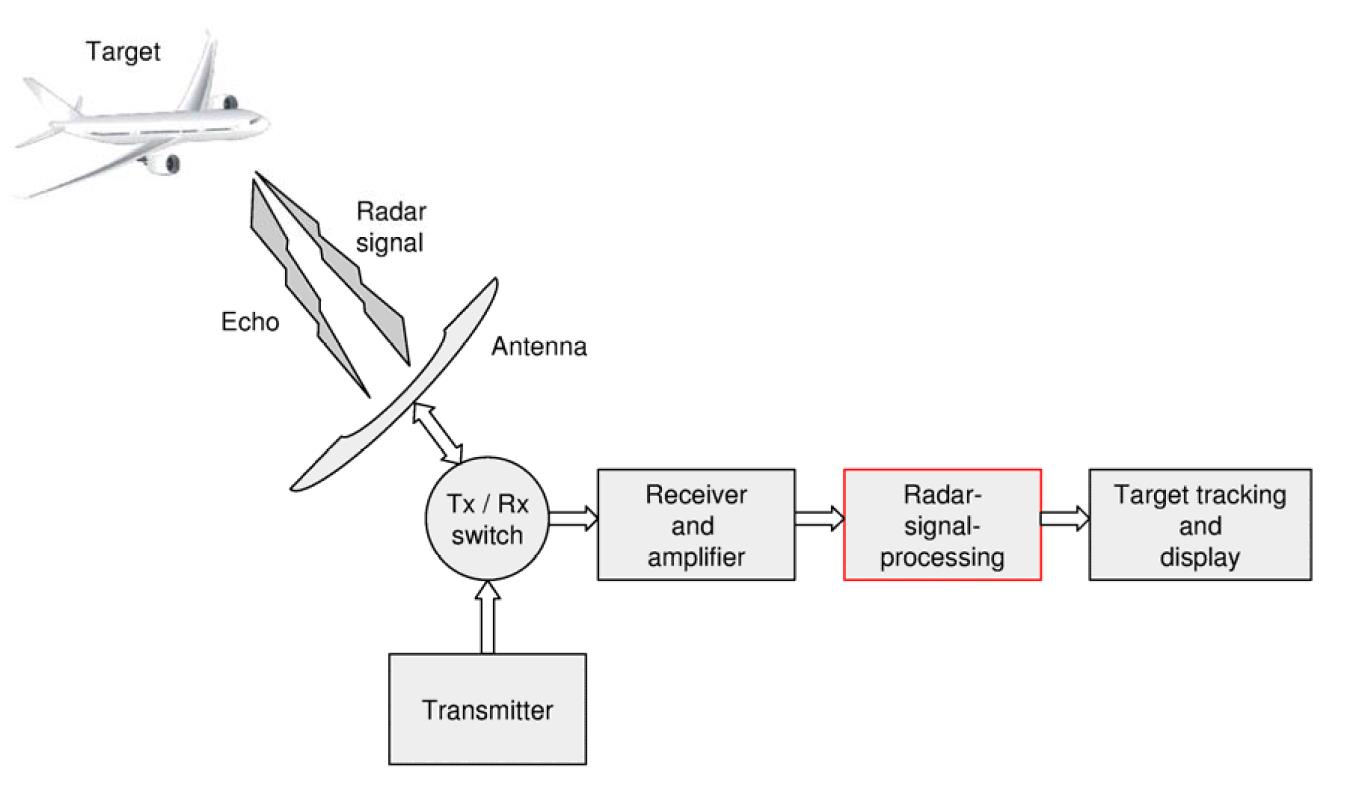
\includegraphics[width=130mm, height=75mm]{figures/radar_principle}
	\caption{Block Diagram of Pulse Doppler Radar \cite{Ludl}}
	\label{fig:intro:radar:blockdia}
\end{figure}

The time delay between sending the pulse and receiving the echo reveals the distance to the target. The frequency shift in the echo tells the radial velocity of the target.
\begin{figure}[h!]
	\centering
	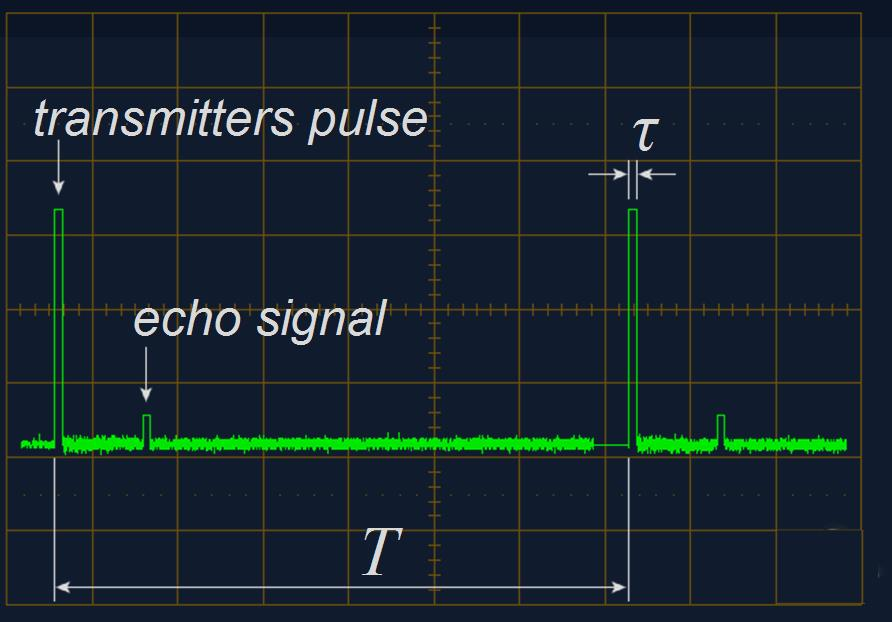
\includegraphics[width=75mm]{figures/trRx}
	\caption{Transmitter's Pulse and Echo Signal from Target \cite{radarTut}}
	\label{fig:intro:radar:txrx}
\end{figure}

Conventional waveband format is followed by manufacturers to address the radar operating frequency. Nowadays, radars are operated from 300MHz to 100GHz in different wavebands. The purpose and installation location of the radar determines the waveband. The accuracy of the radar is proportional to the operating frequency. Also, high frequency signals are more attenuated to water droplets and water vapours in the atmosphere. On the other hand, attenuation of the lower frequency signals is lower than high frequency signals. The typical use case of low frequency radar is in Early Warning Systems whereas high frequency radars are deployed in missile guidance systems \cite{radarExample}.

\subsection{Terminologies}
Radar systems use the spherical coordinate system to localize an object in the sky. The three following information are required to pin point an object relative to the Radar's position.

\textsl{\textbf{Azimuth angle ($\theta _{az}$):}} It is the angle between north and the target in horizontal plane. Azimuth angle can say whether the target is in the left side or right side to the north.

\textsl{\textbf{Elevation angle ($\varphi _{el}$):}} It is the angle between the target and Radar's local plane. Elevation says altitude of the target relative to the Radar. The Azimuth angle and Elevation angle of the Sun are explained in Figure \ref{fig:intro:radar:aziele}.

\textsl{\textbf{Radial distance (r):}} Distance between the target and Radar.\\

\begin{figure}[h!]
	\centering
	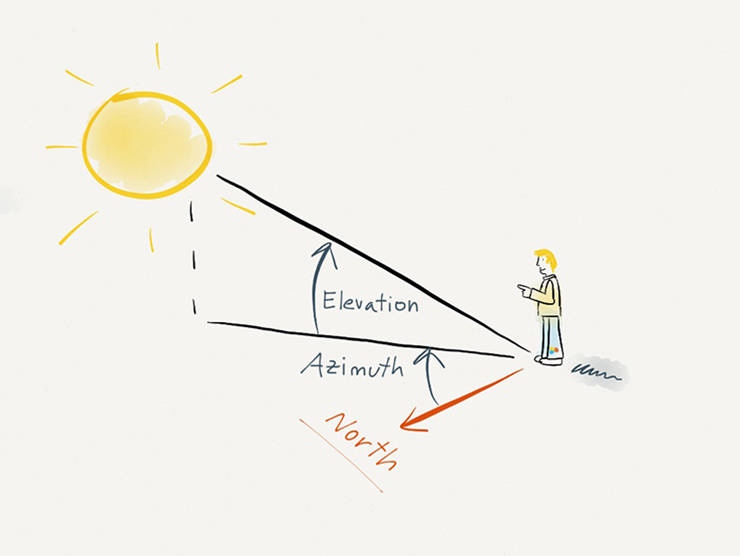
\includegraphics[width=75mm]{figures/azimuth_elevation}
	\caption{Azimuth and Elevation of the Sun \cite{aziEle}}
	\label{fig:intro:radar:aziele}
\end{figure}
\noindent
Other terminologies related to this thesis are explained here. \\[0.4cm]
\textsl{\textbf{Pulse:}} The Radar transmits an electromagnetic signal for a short duration (T$_{on}$) called pulse, then a break (T$_{off}$) follows to receive the echo of the pulse. This T$_{on}$ and T$_{off}$ together is called Pulse Repetition Time (PRT). Actual frequency of the electromagnetic wave transmitted during T$_{on}$ period is called carrier frequency.\\[0.2cm]
%\vspace*{0.2cm}
\noindent
\textsl{\textbf{Burst:}} The Radar sends $n$ number of pulses and listens to the echo signal. The combination of the selected PRT and the number of pulses are called Burst. Figure \ref{fig:intro:radar:prf} shows two different bursts having 3 pulse count each.

\begin{figure}[h!]
	\centering
	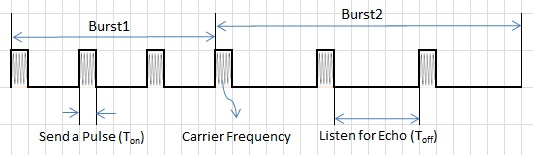
\includegraphics[]{figures/prf}
	\caption{Example of Burst}
	\label{fig:intro:radar:prf}
\end{figure}
\vspace*{0.2cm}
\noindent
\textsl{\textbf{PRF:}} Inverse of Pulse Repetition Time is called Pulse Repetition Frequency. \\
\noindent
\textsl{\textbf{Dwell:}} Group of 8 different bursts form a Dwell.
\FloatBarrier
\noindent
\textsl{\textbf{Range Gate:}} The received  echo signal is sampled at given time intervals called as range gates, shown in Figure \ref{fig:intro:radar:rg}. They represent distance from the Radar transmitter.

\begin{figure}[h!]
	\centering
	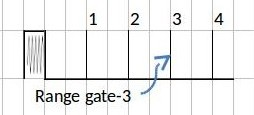
\includegraphics[width=60mm]{figures/range_gate}
	\caption{Example of Range Gate}
	\label{fig:intro:radar:rg}
\end{figure}
\noindent
\textsl{\textbf{Air to Air Mode (A/A Mode):}} The Radar mounted on an aircraft, scanning the sky.\\
\noindent
\textsl{\textbf{Air to Ground Mode (A/G Mode):}} The Radar mounted on an aircraft, scanning the Ground.
%%%%%%%%%%%%%%%%%%%%%%%%%%%%%%%%%%%%%
%%%%%%%%%%%%%%%%%%%%%%%%%%%%%%%%%%%%%
%%%%%%%%%%%%   SECTION   %%%%%%%%%%%%
%%%%%%%%%%%%%%%%%%%%%%%%%%%%%%%%%%%%%
%%%%%%%%%%%%%%%%%%%%%%%%%%%%%%%%%%%%%
\section{Motivation}
\label{sec:intro:motivation}
Radar is one of the core components of a combat air system. Range and accuracy of the Radar are important for missile system, guidance system, early warning system, etc. Massively parallel processor arrays, DSP processors, FPGA processors and GPU processors\cite{HalmSwe} are some examples of the Radar processors in the industry.  They demand high computation capabilities, more power and so big in size.

Avionics and military applications always thrives to minimize the Size, Weight and Power (SwaP) while demanding high performance. It remains the backbone of the research. This thesis explores the possibilities of bringing a new dimension to the low cost and real-time Radar processor that can be employed in safety critical systems. ARM processor, which is running in millions of smart devices\cite{armWeb} is chosen, keeping compactness, portability and power requirements in mind. As a first step, medium range (40nm) Radars are considered as a suitable candidates to adopt low cost and compact ARM processors, since they do not need several TFLOP of processing power to adhere the real-time requirements.

A baseline analysis is carried out by Airbus DS concludes that the ARM processors cannot meet the real-time requirements, if the scheduling of the Radar processing algorithm not optimized. This thesis extends the baseline analysis and implements a couple of optimized scheduling schemes to meet the real-time requirements. The results of the optimized schemes and possible improvements are discussed in detail.

%%%%%%%%%%%%%%%%%%%%%%%%%%%%%%%%%%%%%
%%%%%%%%%%%%%%%%%%%%%%%%%%%%%%%%%%%%%
%%%%%%%%%%%%   SECTION   %%%%%%%%%%%%
%%%%%%%%%%%%%%%%%%%%%%%%%%%%%%%%%%%%%
%%%%%%%%%%%%%%%%%%%%%%%%%%%%%%%%%%%%%
\section{Requirements of the Radar Processor}
\label{sec:intro:realtime_req}
A Radar mounted on an aircraft or satellite is called Airborne Radar. The Airborne Radar processor should be able to process Air to Air (A/A) Mode data and Air to Ground Mode (A/G) data. As the Radar processor is a part of a safety critical system, it should stick to the industrial standards DO-178B/C, ARINC-653.

Since this research is in the early stage of development, and to allow room for further requirements, the CPU utilization is restricted to 50\% of the available CPU time, memory utilization should be less than 50\% of the available memory size and the peak data transfer rate of the Radar application should be less than 50\% of the maximum achievable data transfer bandwidth. The real-time requirements of the Radar processor shall be summarized as follows
\begin{itemize}
        \itemsep0em
        \item \textit{Resulting processing latency:} The time span between reception of an echo and the processed information is sent out, should be less then 2x Dwell time.
        \item \textit{Memory transfer bandwidth:} <50\%.
        \item \textit{Memory utilization:} <50\%.
        \item \textit{CPU utilization:} <50\%.
\end{itemize}


%%%%%%%%%%%%%%%%%%%%%%%%%%%%%%%%%%%%%
%%%%%%%%%%%%%%%%%%%%%%%%%%%%%%%%%%%%%
%%%%%%%%%%%%   SECTION   %%%%%%%%%%%%
%%%%%%%%%%%%%%%%%%%%%%%%%%%%%%%%%%%%%
%%%%%%%%%%%%%%%%%%%%%%%%%%%%%%%%%%%%%
\section{Problem Statement}
\label{sec:intro:probstatement}
The Airborne Radar is subjected to operate on different Pulse Repetition Frequencies (PRF) to resolve ambiguity in distance and velocity. Consecutive eight different bursts form a Dwell. That is, on every time the Radar probes the sky, it sends one Dwell and the echoes are received and analysed. The resulting processing latency of the baseline analysis is theoretically calculated as 15x Dwell time (see Table \ref{tbl:mm:scheme1_true_latency}).  It means, to produce the result of the first Dwell, it needs as much time as the 15 Dwell transmission require. A typical Dwell time is 54ms. An Euro-fighter Typhoon moving at a speed of Mach 2 would move a distance of 560 meters during this processing time. Half a kilometre difference between detection and display is very high for a typical Airborne Radar processor.

The real-time requirement confines the processing latency to 2x Dwell time. The investigation of this thesis is to find an optimal scheduling scheme, number of processors required, data distribution, resulting processing latency and exploit the parallelism in the Radar processing algorithm to stick to the real-time requirements.

%%%%%%%%%%%%%%%%%%%%%%%%%%%%%%%%%%%%%
%%%%%%%%%%%%%%%%%%%%%%%%%%%%%%%%%%%%%
%%%%%%%%%%%%   SECTION   %%%%%%%%%%%%
%%%%%%%%%%%%%%%%%%%%%%%%%%%%%%%%%%%%%
%%%%%%%%%%%%%%%%%%%%%%%%%%%%%%%%%%%%%
\section{Contributions}
\label{sec:intro:contrib}
One of the major works of this thesis is, binding the performance critical functional blocks of the Radar processing algorithm, to replicate the Radar processing chain, targeting multi-core architecture and multi-threaded application. In summary, the main contributions of this thesis are:

\begin{itemize}
\item{\bf Multi-core Performance}
  \begin{itemize}
    \item Scalability and performance of the application on multi-core environment are estimated. Shared resources, resource contention and race condition are considered.
    \item All the threads are set to execute the functional blocks simultaneously to ensure the maximum memory transfer bandwidth.
  \end{itemize}
\item {\bf Scheduling Scheme}
 	\begin{itemize}
 	\item Data dependencies are identified and evaluated by executing them in parallel using POSIX Threads.
   	\item Constraints on non-thread-safe functional blocks are identified and scheduled them without violation.
   	\item Optimal scheduling schemes are proposed and their results are assessed.
	\end{itemize}
\item {\bf Measurement Tools}
  \begin{itemize}
      \item Developed automated scripts to measure peak memory utilization, CPU utilization, memory transfer bandwidth and processing latency.
  \end{itemize}
\end{itemize}

%%%%%%%%%%%%%%%%%%%%%%%%%%%%%%%%%%%%%
%%%%%%%%%%%%%%%%%%%%%%%%%%%%%%%%%%%%%
%%%%%%%%%%%%   SECTION   %%%%%%%%%%%%
%%%%%%%%%%%%%%%%%%%%%%%%%%%%%%%%%%%%%
%%%%%%%%%%%%%%%%%%%%%%%%%%%%%%%%%%%%%
\section{Thesis Outline}
\label{sec:intro:outline}

The rest of this thesis is organized as follows:

%\begin{compactitem}
\begin{itemize}
	\item \textbf{Chapter \ref{chap:bg_related_work}:} Explains the Integrated Modular Avionics (IMA) architecture, experimental set-up and related work concerning ARM processors in Radar application.

	\item \textbf{Chapter \ref{chap:existing_analysis}:} Discusses the results of the baseline analysis done by Airbus Defence and Space GmbH.

	\item \textbf{Chapter \ref{chap:testbed}} Explains the pros and cons of the baseline analysis, test bed information and important design choices.

	\item \textbf{Chapter \ref{chap:mode_mapping}:}  Proposes optimized scheduling schemes and verifies their correctness via implementation. Results of the new schemes are discussed.

	\item \textbf{Chapter \ref{chap:conclusion}:} Summarizes this thesis with a conclusion and proposes future work regarding the optimized schemes.
\end{itemize}
%


%%%%%%%%%%%%%%%%%%%%%%%%%%%%%%%%%%%%%%%%%%%%%%%%%%%%%%%%%%%%%%%%%%%%%%%%%%
%%%%%%%%%%%%   CAPTER 2   %%%%%%%%%%%%%%%%%%%%%%%%%%%%%%%%%%%%%%%%%%%%%%%%
%%%%%%%%%%%%%%%%%%%%%%%%%%%%%%%%%%%%%%%%%%%%%%%%%%%%%%%%%%%%%%%%%%%%%%%%%%
\chapter{Background and Related Work}
\label{chap:bg_related_work}
Minimizing size, weight and power consumption of the Radar processor without compromising performance is the topic under research. The low cost, portable processor is intended for weight and power limited airborne platform such as Unmanned Airborne Vehicles. On satisfactory performance, this may open doors for new business opportunities in Radar processing and safety critical applications. \\
ARM is the favourable architecture in this regard, and has been running in millions of smart phones, tablets and portable gadgets. Instead of one high capacity, power hungry, bulk processor, several small, energy efficient, compact processors of ARM type can be deployed. The way of grouping the processors, experiment setup \footnote{These information are based on the technical documentation provided by Airbus Defence and Space GmbH, titled \textsl{Future Combat Air System - Analysis of IMA Modules,} version B.} and state of the art related work are elaborated in this chapter.

%%%%%%%%%%%%%%%%%%%%%%%%%%%%%%%%%%%%%
%%%%%%%%%%%%%%%%%%%%%%%%%%%%%%%%%%%%%
%%%%%%%%%%%%   SECTION   %%%%%%%%%%%%
%%%%%%%%%%%%%%%%%%%%%%%%%%%%%%%%%%%%%
%%%%%%%%%%%%%%%%%%%%%%%%%%%%%%%%%%%%%
\section{IMA Processor Architecture} 
\label{sec:bg_related_work:ima}
Integrated Modular Avionics is the cluster of real-time computing elements capable of executing multiple tasks having different safety critical levels. Instead of several dedicated computers for different purposes, a common hardware platform for many systems is used. This improves fault isolation, increased airborne functionality and ability to move applications between standardized computers \cite{theAvionics}. To comply with the environmental requirements, industrial temperature standard, MCIMX6Q7CVT08AC processor type with 800MHz clock speed is used. \\

IMA architecture comprises of the following modules \footnote{SPM Module and iCON Module are out of this thesis scope.}
\begin{compactitem} 
	\item up to 2 Platform Support Modules (PSM) 
	\item up to 6 Data Graphics Processing Module (DGPM) or Signal Processing Module (SPM) or any combination of these two.
	\item up to 3 Interface Concentrator Module (iCON).
	\item a rack backplane.
\end{compactitem}

%%%%%%%%%%%%%%%%%%%%%%%%%
%%%%%   SUB-SECTION   %%%
%%%%%%%%%%%%%%%%%%%%%%%%%
%%%%%%%%%%%%%%%%%%%%%%%%%
\subsection{Platform Support Modules (PSM)}
\label{ss:bg_related_work:psm}
The PSM has the following components:
\begin{compactitem} 
	\item one iMX6Q CPU, clocked 800MHz.
	\item one 1GBit/s-Ethernet switch with 10 bi-directional communication ports.
	\item CPU has it's own private 4GiB SDRAM and non-volatile NOR/NAND Flash memory.
	\item 16GiB Solid State Disk, connected to the CPU via SATA interface.
\end{compactitem}

\begin{figure}[h!]
	\centering
	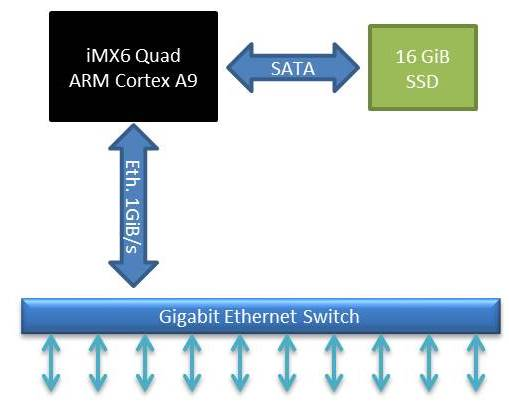
\includegraphics[width=90mm]{figures/psm}
	\caption{Platform Support Module \cite{fcas}}
	\label{fig:bg_related_work:ima:psm}
\end{figure}

The PSM Module acts as a router between different modules of the Radar processor. It directs the Radar raw data to an apt processing module (DGPM or SPM) and send the processing result to a target display module.

%%%%%%%%%%%%%%%%%%%%%%%%%
%%%%%   SUB-SECTION   %%%
%%%%%%%%%%%%%%%%%%%%%%%%%
\subsection{Data Graphics Processing Module (DGPM)}
\label{ss:bg_related_work:dgpm}
The DGPM has the following characteristics:
\begin{compactitem} 
	\item 4 iMX6Q CPUs, clocked 800MHz.
	\item one 1GBit/s-Ethernet switch with 6 bi-directional communication ports.
	\item each of the 4 CPUs has it's own private 4GiB SDRAM and non-volatile NOR/NAND Flash.
memory \\
\end{compactitem}

\begin{figure}[h!]
	\centering
	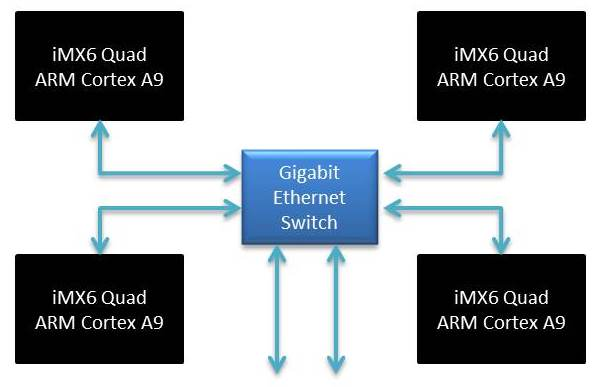
\includegraphics[width=100mm]{figures/dgpm}
	\caption{Data Graphics Processing Module \cite{fcas}}
	\label{fig:bg_related_work:ima:dgpm}
\end{figure}

The iMX6Q6 CPU has four identical ARM Cortex A9 cores with Advanced SIMD unit (NEON), 32KiB I and D-cache, one unified 1MiB L2-cache shared by 4 cores, smart DMA, 3D and 2D Graphics Processing Unit, one common 533MHz 64-bit DDR3 memory interface, one common 1GBit/s Ethernet interface and several other standard interfaces \cite{imx_spec}, (Appendix \ref{app:imx6q}). The SPM Module has not been considered due to the decision of Airbus DS.

%%%%%%%%%%%%%%%%%%%%%%%%%
%%%%%   SUB-SECTION   %%%
%%%%%%%%%%%%%%%%%%%%%%%%%
\subsection{Radar Processor Design}
\label{ss:bg_related_work:togther}
As shown in Figure \ref{fig:bg_related_work:ima:radar_processor}, the received raw data will undergo the following stages to be transformed as desired information.
\begin{enumerate}
	\item Radar receiver front-end sends the received data to the iCON1 Module along with supplementary information like antenna azimuth, antenna elevation, etc. Data distribution to the PSM modules is controlled by the iCON1. 

	\item PSM1 and PSM2 routes the received data to the pre-defined DGPM modules. Routing mechanism can be reconfigured.

	\item As soon as the DGPM has completed processing, data will be sent back to the respective PSM module.

	\item PSM routes the processed data to iCON2. 

	\item iCON2 routes the processed A/A Mode data, SAR Mode data to the tracking processor, display processor respectively. 
\end{enumerate}
Nominal data transfer rate of the communication links are 1GBit/s. Booting the software can be done from SSD or remotely via an appropriate system interface.

\begin{figure}[h!]
	\centering
	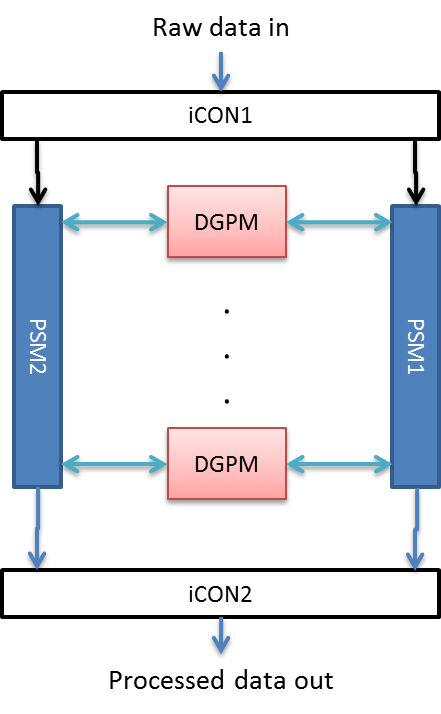
\includegraphics[]{figures/radar_processor}
	\caption{Block Diagram of Radar Processor \cite{fcas}}
	\label{fig:bg_related_work:ima:radar_processor}
\end{figure}

%%%%%%%%%%%%%%%%%%%%%%%%%%%%%%%%%%%%%
%%%%%%%%%%%%%%%%%%%%%%%%%%%%%%%%%%%%%
%%%%%%%%%%%%   SECTION   %%%%%%%%%%%%
%%%%%%%%%%%%%%%%%%%%%%%%%%%%%%%%%%%%%
%%%%%%%%%%%%%%%%%%%%%%%%%%%%%%%%%%%%%
\section{Experiment Set-up}
\label{s:bg_related_work:exp_setup}
A Nitrogen6X development kit is used to match the basic building block of the IMA processor architecture, which is iMX6Quad processor, clocked 1GHz. The communication to the Nitrogen6X board is carried via Ethernet interface. Measurements of the processing latency is performed on the target and exported in \bverb|.csv| format. The results are scaled down to 800MHz to match the IMA architecture. Scheduling schemes and processing latency analysis are based on the single iMX6Quad processor result, measured from the Nitrogen6X board.

%%%%%%%%%%%%%%%%%%%%%%%%%
%%%%%   SUB-SECTION   %%%
%%%%%%%%%%%%%%%%%%%%%%%%%
\subsection{Target Hardware}
\label{ss:bg_related_work:hw}
The target hardware is a Nirtogen6X development board (Appendix \ref{app:nitrogen6x}) from Boundary Devices Inc. It is a low cost development kit built with iMX6Quad processor. Some of it's features are:
\begin{compactitem} 
	\item Quad-Core ARM Cortex A9 processor clocked 1GHz
	\item 1GiB of 64-bit wide DDR3 at 532MHz
	\item Three display ports (RGB, LVDS and HDMI)
	\item Serial ATA 2.5 (SATA) at 3GBit/s
	\item Dual SD 3.0/SDXC card slots
	\item 10/100/1000 Ethernet
	\item 10-pin JTAG interface
	\item High speed USB ports (2xHost, 1xOTG)
	\item Real-Time Clock with battery backup
\end{compactitem}

%%%%%%%%%%%%%%%%%%%%%%%%%
%%%%%   SUB-SECTION   %%%
%%%%%%%%%%%%%%%%%%%%%%%%%
\subsection{Software Development Platform}
\label{ss:bg_related_work:sw}
Linaro Linux is installed on the Nitrogen6X board along with Lightweight X11 Desktop Environment. Functional blocks of the Radar processing algorithm are written in \bverb|C|. Other details are:

\begin{compactitem} 
	\item \bverb|Linaro Linux 3.0.35-02828-g5cedf96| is installed on Nirtogen6X board.
	\item Software Development Environment: Eclipse CDT Version: 3.8.0.
	\item C compiler: \bverb|gcc Debian 4.7.2-5|.
	\item Cross compiler: \\ARM A9 cross-compiler \bverb|gcc-linaro-arm-linux-gnueabihf-4.8-2013.09_linux|.
	\item Other application library: FFTW 3.3.3 \cite{fftw}. \\
\end{compactitem} 

\lstset{ %
  backgroundcolor=\color{mildyellow},   % choose the background color; you must add \usepackage{color} or \usepackage{xcolor}
  breakatwhitespace=false,         % sets if automatic breaks should only happen at whitespace
  breaklines=true,                 % sets automatic line breaking
  keepspaces=true,                 % keeps spaces in text, useful for keeping indentation of code (possibly needs columns=flexible)
  numbers=none,                    % where to put the line-numbers; possible values are (none, left, right)
  showspaces=false,                % show spaces everywhere adding particular underscores; it overrides 'showstringspaces'
  showstringspaces=false,          % underline spaces within strings only
  basicstyle=\ttfamily\small,
  frame=single,
}

%%%%%%%%%%%%%%%%%%%%%%%%%%%%%%%%%%%%%
%%%%%%%%%%%%%%%%%%%%%%%%%%%%%%%%%%%%%
%%%%%%%%%%%%   SECTION   %%%%%%%%%%%%
%%%%%%%%%%%%%%%%%%%%%%%%%%%%%%%%%%%%%
%%%%%%%%%%%%%%%%%%%%%%%%%%%%%%%%%%%%%
\section{Air to Air Mode Processing Chain}
\label{sec:bg_related_work:proc_chain}
Previous work has been carried out by Airbus DS in Future Combat Air System (FCAS) project, see \cite{fcas}. This section is an excerpt of the FCAS project, describes the Radar processing chain to understand the rest of the thesis.

At first, the Radar system in the flight scans the sky $\pm$60$^{\circ}$ from boresight. The azimuth scan of the antenna is sub-divided into 2 x 5 angular segments, called look directions (5 segments in the positive half and 5 segments in the negative half of the scan width). Given the beam width of 2.5$^{\circ}$, 48 beams are required to cover the 120$^{\circ}$ space. Figure \ref{fig:bg_related_work:aa_look_dir} explains the 5 look direction segments in positive half of the azimuth scan. The Air to Air Mode has different PRF set for different look directions. The PRF and range gate configuration determines the amount of input data to the Radar processor. Table \ref{tbl:aa_exe} shows the maximum execution time of the Radar functions running on a single core, 1GHz iMX6Quad processor. The baseline analysis scales down the results to 800MHz to match the IMA processor architecture.

\begin{figure}[h!]
	\centering
	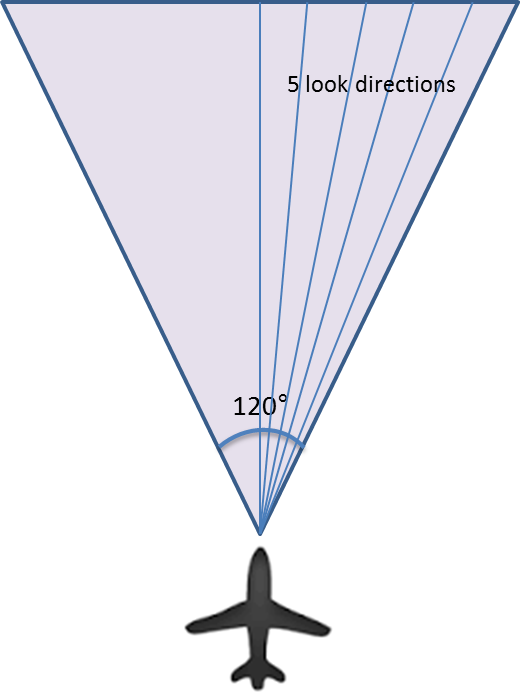
\includegraphics[width=55mm]{figures/look_dir}
	\caption{Details of the A/A Mode Scan}
	\label{fig:bg_related_work:aa_look_dir}
\end{figure}

The Radar antenna has 8 transmit and receive channels and 1 guard channel. The guard channel works as a detector to distinguish main-lobe echoes and side-lobe echoes. Every scan consists several Dwells. All the Dwells are independent. The A/A Mode processing is done independently for each Dwell. It comprises of the following stages.\footnote{This section only describes an overview of the algorithm, since the algorithm is classified as Airbus DS Confidential.}

\begin{figure}[h!]
	\centering
	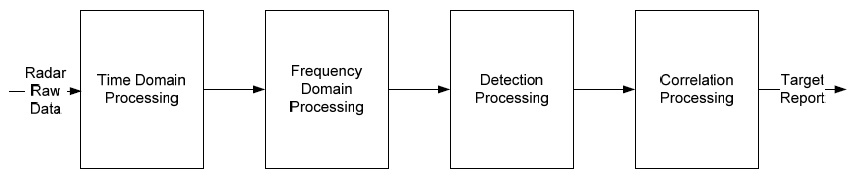
\includegraphics[width=160mm]{figures/aa_block_dia}
	\caption{Block Diagram of Air to Air Mode Processing}
	\label{fig:bg_related_work:aa_block_dia}
\end{figure}

\subsection{Time Domain Processing}
Beam-forming is a Digital Signal Processing technique that allows the Radar transceiver to focus on a particular direction. Beam-forming has to be performed for Sum channel($S_{S}$), Azimuth channel($S_{AZ}$) and Elevation channel($S_{EL}$). During Sum channel beam-forming, the input vectors of 8 antenna receive channels are multiplied with pre-calculated Sum channel beam-forming vectors. The resulting vectors are added to produce a Sum channel beam. This step is repeated for Azimuth channel and Elevation channel. Guard (9$^{th}$) channel doesn't require beam-forming, only requires float conversion. Each of the processed four channel data are multiplied by pre-calculated weighting vector. 

Digital Pulse Compression, also called Convolution, is computation expensive in time domain, so it is performed in frequency domain. Convolution in time domain is multiplication in frequency domain, it is performed channel by channel by computing FFT, Multiplication followed by IFFT.

\begin{figure}[h!]
	\centering
	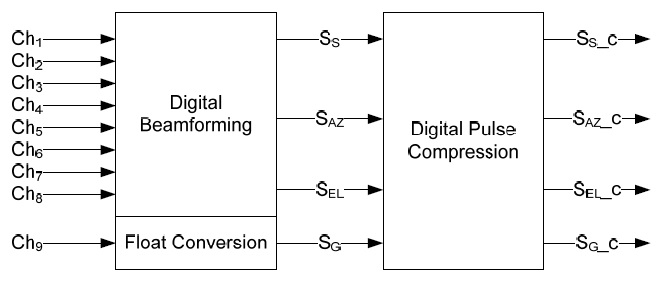
\includegraphics[width=120mm]{figures/aa_tdp}
	\caption{A/A Mode Time Domain Processing}
	\label{fig:bg_related_work:aa_tdp}
\end{figure}

\subsection{Frequency Domain Processing (FDP)}
Each channel pulse compressed data is in the form of [pulse x range] matrix. Frequency domain tranformation has to be applied on the data corresponding to the same range gates of different pulse. So the pulse compressed data shall be corner turned to [range x pulse] matrix as shown in Figure \ref{fig:bg_related_work:cot}, then FFT is computed for the Sum, Guard, Azimuth and Elevation channel followed by magnitude of the Sum channel and Guard channel are computed.

\begin{figure}[h!]
	\centering
	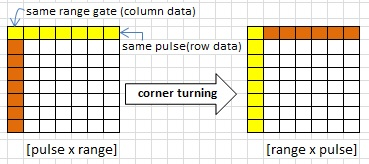
\includegraphics[]{figures/cot}
	\caption{Corner Turning}
	\label{fig:bg_related_work:cot}
\end{figure}

\begin{figure}[h!]
	\centering
	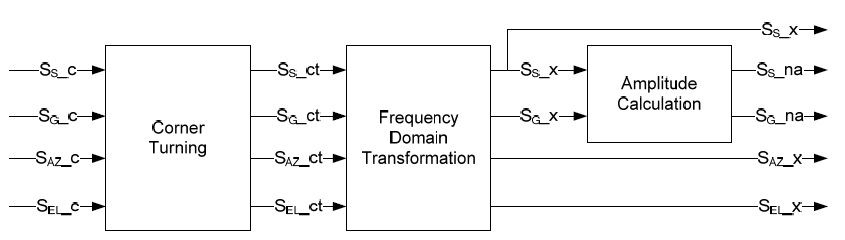
\includegraphics[width=140mm]{figures/aa_fdp}
	\caption{A/A Mode Frequency Domain Processing}
	\label{fig:bg_related_work:aa_fdp}
\end{figure}

\subsection{Detection Processing (DET)}
Area threshold of the individual elements in the Sum channel and the Guard channel are determined by computing average of the surrounding elements values. An additional pre-alarm matrix is computed by comparing the amplitude matrix and the area threshold matrix. The pre-alarm says the detection may be a potential target. If the element in the amplitude matrix is greater than the corresponding element in the threshold matrix, pre-alarm is set TRUE in the corresponding pre-alarm matrix, otherwise pre-alarm element is set to FALSE. To prevent the Sum channel alarms caused by side-lobe entries, it is compared with the Guard channel alarms. \\The number of alarms are limited by the N$_{max\_alarms}$ with the shortest range from the list called Constant False Alarm Rate(CFAR). Alarm list is generated by referring the pre-alarm matrix and corresponding Sum, Azimuth, Elevation channel values.\\

\begin{figure}[h!]
	\centering
	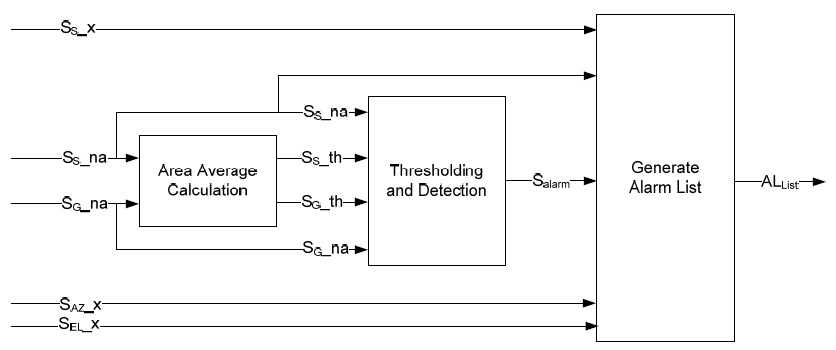
\includegraphics[width=140mm]{figures/aa_det}
	\caption{A/A Mode Detection Processing}
	\label{fig:bg_related_work:aa_det}
\end{figure}

\subsection{Correlation Processing}
This stage resolves the ambiguity in distance and velocity by comparing the current burst data with 7 previous bursts. Correlation processing is not considered as a performance critical module and hence this stage is not benchmarked. 

\begin{figure}[h!]
	\centering
	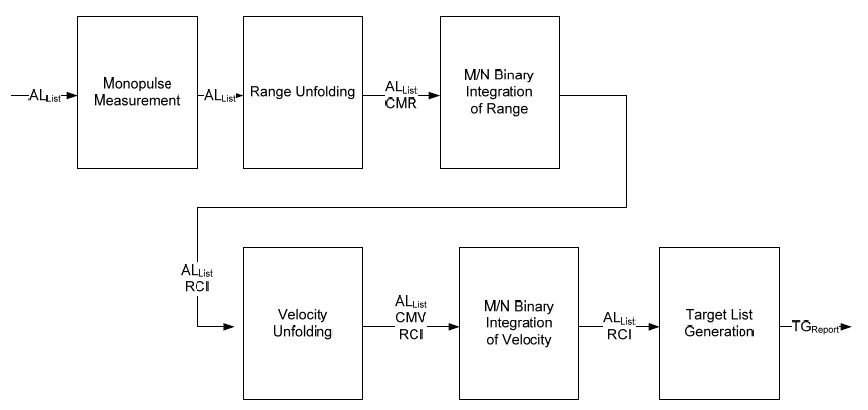
\includegraphics[width=140mm]{figures/aa_corr}
	\caption{A/A Mode Correlation Processing}
	\label{fig:bg_related_work:aa_corr}
\end{figure}
\FloatBarrier

\section{A/A Mode Sequence of Execution}
\label{sec:ch2:benchmark_results}
Performance critical functions related to the Radar processing algorithm are identified by Airbus DS. The functional blocks are executed in the iMX6Quad processor, clocked 1GHz and their execution times are listed in Table \ref{tbl:aa_exe}. The functional block 100CMYACC8, multiplies each element of a [100 x 8] element complex matrix with an 8-element complex vector and accumulate the 8 complex multiplication results to a single complex result, resulting in a [100 x 1] element complex matrix. Explanation about the other functional blocks can be found in Appendix \ref{description:benchmark}.

\begin{longtable}{|l|l|l|}
		\hline
		\textbf{Functional Block} & \textbf{\#cycles in iMX6Quad processor} & \textbf{Unit}  \TBstrut \\ \hline
		100CMYACC8 & 79 & per 8 element \TBstrut \\ \hline
		100RMY50 & 15 & per complex element \TBstrut \\ \hline
		100CONV128 & 24100 & per 128-pt vector \TBstrut \\ \hline
		150COT50 & 12 & per complex element \TBstrut \\ \hline
		100FFT64 & 2,550 & per 64-pt vector \TBstrut \\ \hline
		50MAG256 & 20 & per complex element \TBstrut \\ \hline
		64AVG100 & 20 & per element \TBstrut \\ \hline
		64CMPR100 & 7 & per element \TBstrut \\ \hline
		64DET100 & 10 & per element  \TBstrut \\ \hline
		\caption{Measured Execution Cycles of the Functional Blocks}
		\label{tbl:aa_exe}
\end{longtable}

The functional blocks shall be executed as shown in Figure \ref{fig:bg_related_work:aa_seq} to mimic the Radar processing chain. Functions of the Correlation processing are not included here. In the following figure, \textsl{3x CMYACC} means, computing \hyperlink{benchmarks}{CMYACC} for three channels ($S_{S},S_{AZ},S_{EL}$).

\begin{figure}[h!]
	\centering
	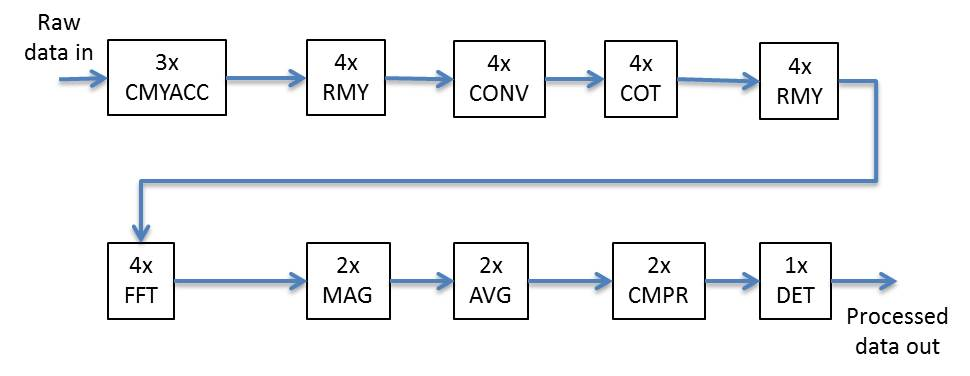
\includegraphics[width=160mm]{figures/aa_seq}
	\caption{A/A Mode, Sequence of Functional Blocks Execution}
	\label{fig:bg_related_work:aa_seq}
\end{figure}

STREAM benchmark\cite{McCalpin2007} is used to measure memory bandwidth of a machine. The STREAM benchmark is a simple, synthetic benchmark designed to measure sustainable memory bandwidth (in MB/s) and a corresponding computation rate for four simple vector kernels namely Copy, Scale, Add and Triad \cite{streamDef}. According to the STREAM benchmark, 400 MiB/s data transfer rate is measured while copying data from one memory location of the SDRAM to another memory location, when a single core is active (2cycle/byte). L2 cache to SDRAM data transfer rate of 350MiB/s (2.29cycle/byte) is measured when all the four cores are active. Operating System overhead is assumed as the factor of 1.3 to carry out the execution. Cycle time of the core is 1.25ns, as it is running at 800MHz frequency. Execution cycle for the Correlation processing is heuristically assumed as follows.


\begin{table}[h!]
	\centering
	\begin{tabular}{|l|l|l||l|l|} 
	 	\hline
		\textbf{Process} & \textbf{\#cycles} & \textbf{Unit} & \textbf{\#cycles} & \textbf{Unit}  \\ \hline
		Monopulse Measurement & 500 & per alarm & - & - \\ \hline
		Range Unfolding & 30 & per range gate & 200 & per alarm \\ \hline
		M/N Binary Integration of Range & 40 & per range gate & 500 & per alarm \\ \hline
		Velocity Unfolding & 30 & per alarm & - & - \\ \hline
		M/N Binary Integration of Velocity & 80 & per alarm & - & - \\ \hline
		Target List Generation & 100 & per target & - & - \\ \hline
	\end{tabular}
	\caption{Execution Cycle of Correlation Processing \cite{fcas}}
	\label{tbl:rel_work:corr_proc_exe}
\end{table}

The execution cycle results listed in the Tables \ref{tbl:rel_work:corr_proc_exe} and \ref{tbl:aa_exe} are the fundamentals for the baseline analysis, explained in the next chapter.
 
%%%%%%%%%%%%%%%%%%%%%%%%%%%%%%%%%%%%%
%%%%%%%%%%%%%%%%%%%%%%%%%%%%%%%%%%%%%
%%%%%%%%%%%%   SECTION   %%%%%%%%%%%%
%%%%%%%%%%%%%%%%%%%%%%%%%%%%%%%%%%%%%
%%%%%%%%%%%%%%%%%%%%%%%%%%%%%%%%%%%%%
\section{Air to Air Mode Radar Characteristics}
\label{ss:aa_mode:radar_char}
Air to Air Mode Radar has the following characteristics. The transmitted carrier frequency is 9GHz and it can detect targets in 40nm range, moving at velocity $\pm$3Mach. A burst shall have a maximum of 32 alarms and a maximum of 16 targets, formed out of the 32 alarms. That is, a burst shall have maximum of 32 detections, of which 16 can be real targets.

\begin{table}
	\centering
	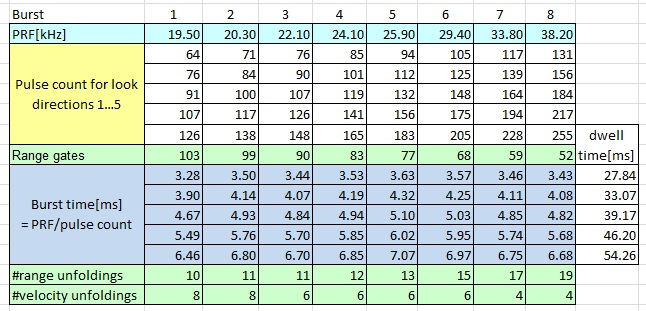
\includegraphics[width=140mm]{figures/aa_char}
	\caption{A/A Mode Radar Characteristics}
	\label{fig:bg_related_work:aa_char}
\end{table}

Figure \ref{fig:bg_related_work:aa_char} shows the detailed information of the Radar system. The first burst of the Look direction-1 consists of 64 pulses transmitted at 19.5 KHz frequency and every pulse shall have 103 range gates. Range unfolding and Velocity unfolding are performed to compute the unambiguous range and unambiguous velocity of the target respectively. They can be mathematically calculated as follows. 

\begin{align*}
	\label{equ:burst_time_calc}
	Dwell \enspace time &= \sum\limits_{n=1}^{8} Burst \enspace time_{n} \\[0.3cm]
	Unambiguous \: Range &= \frac{1}{2} \: \frac{velocity \: of \: the \: radar \: signal}{PRF \: frequency} \\[0.3cm]
	Range \: Unfoldings &= \frac{max.range}{unambiguous \: range} \\[0.3cm]
	Unambiguous \: Velocity &= \frac{1}{2} \frac{velocity \: of \: the \: radar \: signal}{carrier \: frequency} * PRF \: frequency \\[0.3cm]
	Velocity \: unfolding &= 2 * ROUNDUP \bigg( \frac{max.velocity}{unambiguous \: velocity} \bigg ) \\[0.3cm] \stepcounter{equation}\tag{\theequation} 
\end{align*}

%%%%%%%%%%%%%%%%%%%%%%%%%%%%%%%%%%%%%
%%%%%%%%%%%%%%%%%%%%%%%%%%%%%%%%%%%%%
%%%%%%%%%%%%   SECTION   %%%%%%%%%%%%
%%%%%%%%%%%%%%%%%%%%%%%%%%%%%%%%%%%%%
%%%%%%%%%%%%%%%%%%%%%%%%%%%%%%%%%%%%%
\section{Related Work}
\label{sec:related_work}
Deploying ARM processors in fighter aircraft is in the research stage at the moment. Footprints of the low cost Radar processor and optimal scheduling algorithm have been considered as related work of this thesis. Many innovative architectures have been investigated in past to reduce the size, weight and power(SWaP) requirements of the Radar processor. Some of them are discussed below.

In continuation to the bird strike happened in Alaska, a low cost Radar system "eBirdRad" is developed by Tim J. Nohara, et al \cite{relWork1}, focused to detect birds activity in the sky. The Radar uses X-band frequency, 4$^{\circ}$ beam width, 10m resolution, covering 360$^{\circ}$  azimuth angle and 6nm distance. Proprietary Accipiter Radar processor is used for computations. eBirdRad could detect the birds in real time though there are rooms for improvement. It doesn't aim to reduce weight and power requirements, hence it is not a perfect rival for ARM based Radar processors. 

Salama Y, Fitzgerald D et al \cite{relWork3}, have used Wafer Scale Signal Processor(WSSP) for power efficient Radar signal processing. WSSP is a general purpose floating point processor with 4FLOPS/cycle peak performance, consuming 2 to 10 GFLOPS/watt roughly. Simulation results of FFT benchmark shows that up to 3.2FLOPS/cycle can be utilized for 100k FFT size. The WSSP processor has made efforts to reduce power requirements, disregarding size, weight and cost factors.

Research has hit the industry with \textsl{Programmable DSP Cores for Radar Processing}. APTCORE \cite{relWork4}, uses patented processor architecture to efficiently process the Radar benchmarks. It claims to have 3.3x energy efficiency in FFT processing compared to the standard DSPs. According to the documentation, it is compact, low cost, lowest power, scalable and highly configurable. In addition, range and direction processing of 10 sets of 512 values across 16 antennas take 2.3ms at a clock speed of 200MHz. Although the APTCORE has impressive performance in the product brief document, further investigation is required to compare it against ARM Cortex A9's performance.

ARM type processor has been used by Zeng Y, Xu J and Peng D in Velocity Measuring System \cite{relWork2}. Implementation is done in assembly language to take advantage of the pipeline. It uses 24GHz frequency waves and can track the vehicle velocities from 5km/h to 250km/h in 1.5km range. It is a low cost, low power, compact system meant for traffic management.

Cheng C, Chien-Chung C et al \cite{RTsched} proposed a real-time scheduling algorithm which manages resources of a specially designed parallel system, named programmable radar signal processor (PRSP), a special DSP processor. It is designed to be reconfigurable and applicable to most of the Radar systems. It efficiently allocates the tasks to the processing units, but the SwaP features are not addressed.

ZHAN H, YUAN L, and WANG L \cite{RTschedParallel} have proposed an improved allocation algorithm for Radar task allocation in distributed heterogeneous system using Hungarian algorithm. It uses scheduling queue, workload real-time detection and task accumulation threshold to estimate processor workload and allocate the task accordingly. Again, this paper makes better use of the highly capable resources, disregarding SWaP.

The aforementioned researches either concentrate in the direction of ARM processors to realize low cost and compact Radar processor or efficiently scheduling tasks to the available special purpose processors or using dedicated processors. They succeeded in doing so, but they are not meant for safety critical systems with a reasonably good range and resolution and less SWaP. This thesis connects the both ends, taking advantage of less SWaP from ARM processors and optimal scheduling scheme technique from efficient task allocation to bring less SWaP Radar processor for safety critical system.


%%%%%%%%%%%%%%%%%%%%%%%%%%%%%%%%%%%%%%%%%%%%%%%%%%%%%%%%%%%%%%%%%%%%%%%%%%
%%%%%%%%%%%%   CAPTER 3   %%%%%%%%%%%%%%%%%%%%%%%%%%%%%%%%%%%%%%%%%%%%%%%%
%%%%%%%%%%%%%%%%%%%%%%%%%%%%%%%%%%%%%%%%%%%%%%%%%%%%%%%%%%%%%%%%%%%%%%%%%%
\chapter{Baseline Analysis}
\label{chap:existing_analysis}
This chapter explains the baseline analysis carried out by Airbus DS\cite{fcas}. An airborne Radar processor should be capable of processing both the Air to Air Mode data as well as Air to Ground Mode data. The scope of this thesis is limited to A/A Mode processing. Scheduling Schemes in this chapter are based on the timing information provided in the Tables \ref{tbl:aa_exe} and \ref{tbl:aa_exe}. The baseline analysis configures scheduling schemes in accordance to Space Partition and Time Partition.\\ 

\noindent
\textbf{Time Partitioning:}\\
One iMX6Quad CPU is time sliced to run A/A mode and A/G mode alternatively. The timeframe between two subsequent A/A mode execution is called major time frame. Memory and cache are also partitioned for each mode. Intra-partition communication can be done by buffers, semaphores and/or events. When the time slice is completed for Air to Air mode, context switch happens to store the details of A/A Mode and load the details of A/G Mode, afterwards the A/G mode begins execution. Violation of timing behaviour triggers an exception. \\

\noindent
\textbf{Space Partitioning:} \\
A/A mode processing and A/G mode processing are done in separate physical entities. It is the simplest configuration for dedicated data processing. Failure of one of the systems will not affect the other as they are independent. It is assumed that SDRAM and L2 cache are partitioned for 4 cores to improve determinism. Each core has pre-defined accessible address space in Memory and L2 cache. 

%%%%%%%%%%%%%%%%%%%%%%%%%%%%%%%%%%%%%
%%%%%%%%%%%%%%%%%%%%%%%%%%%%%%%%%%%%%
%%%%%%%%%%%%   SECTION   %%%%%%%%%%%%
%%%%%%%%%%%%%%%%%%%%%%%%%%%%%%%%%%%%%
%%%%%%%%%%%%%%%%%%%%%%%%%%%%%%%%%%%%%
\section{Scheme 1 - Space Partitioning}
\label{sec:scheme_1}
A Radar echo received by the Radar antenna is distinguished as A/A mode or A/G mode by the iCON1 module. 
\begin{figure}[h!]
	\centering
	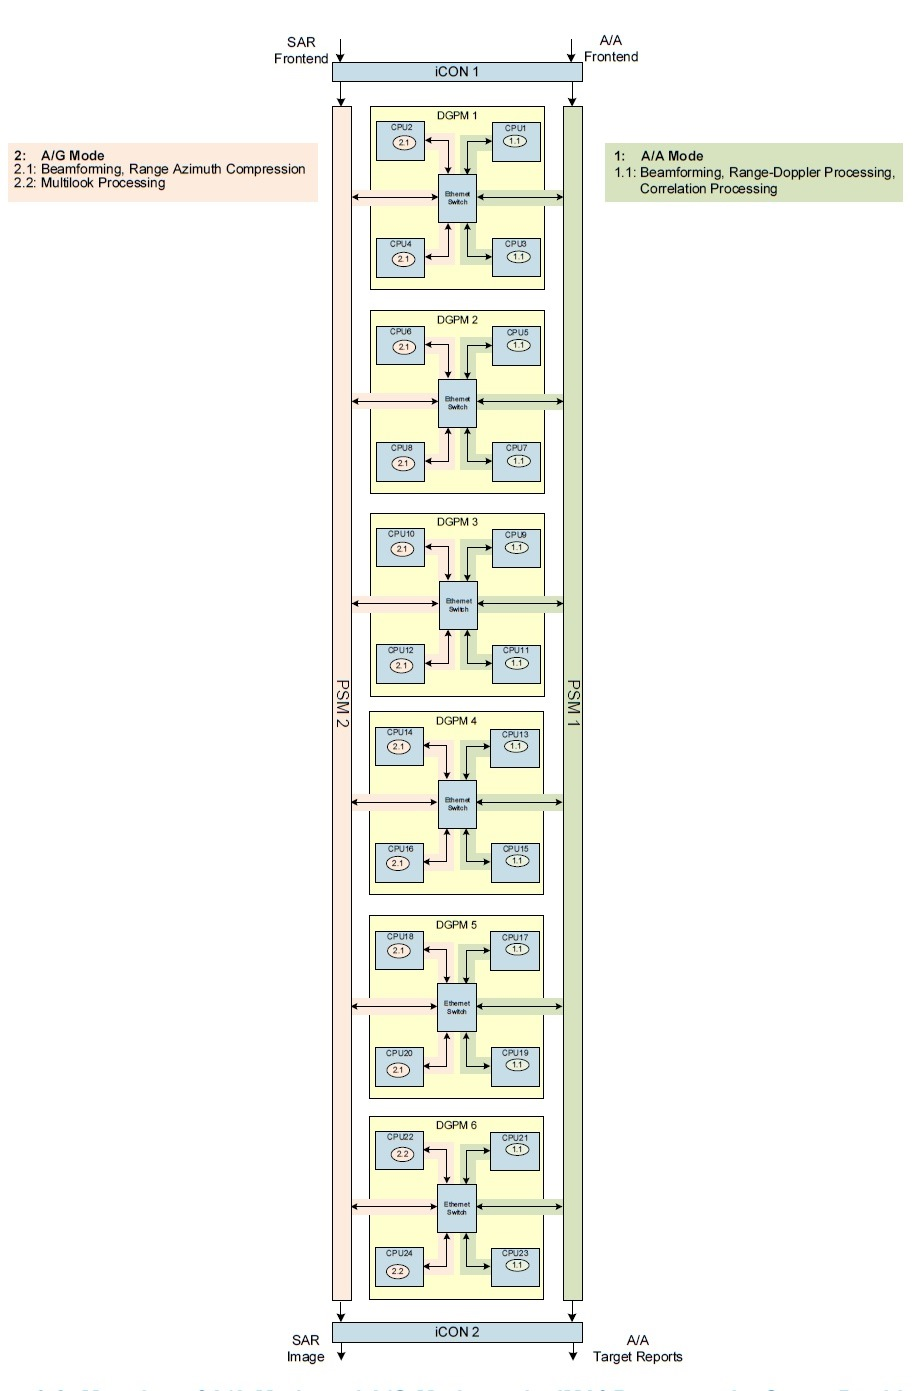
\includegraphics[width=160mm, height=220mm]{figures/scheme1}
	\caption{ Scheduling Scheme}
	\label{fig:existing_analysis:scheme1}
\end{figure}
\FloatBarrier
A/A mode data are redirected to PSM1 and A/G mode data are sent to PSM2. Figure \ref{fig:existing_analysis:scheme1} shows the mapping of A/A Mode and A/G Mode to the IMA processor architecture. The two odd numbered CPUs(CPU1 and CPU3 of DGPM1) of a  DGPM are allocated to the processing of the A/A mode. The two even numbered CPUs(CPU2 and CPU4 of DGPM1)  of a DPGM are allocated to the processing of the A/G mode. Each CPU with it's 4 cores is completely used for either A/A Mode or A/G mode processing.


\begin{tabular}{rl}
	Number of DGPMs: & 6 \\
	Number of CPUs: & 6 x 4 = 24 \\
	CPUs for A/A Mode: & 12 \\
	CPUs for A/G Mode: & 12 \\
\end{tabular}

\noindent
DGPM sends the processed data to iCON2 via respective PSM. iCON2 redirects A/A data to the Tracking processor and A/G data to the Display processor. The SDRAM is assumed to be partitioned for all the four cores, where every core has its buffer memory intended to transfer data between the cores and storage memory to store the data for Radar processing.

%%%%%%%%%%%%%%%%%%%%%%%%%
%%%%%   SUB-SECTION   %%%
%%%%%%%%%%%%%%%%%%%%%%%%%
%%%%%%%%%%%%%%%%%%%%%%%%%
\subsection{A/A Mode Results}
\label{ss:scheme1:aa}
Each CPU processes a Dwell of data. The processing results are dispatched to iCON2 by PSM1. As the Dwell data processing is independent to the processing of the predecessor Dwell data and independent to the processing of the successor Dwell data, there  is no data dependency between CPUs processing different Dwell data.

\begin{figure}[h!]
	\centering
	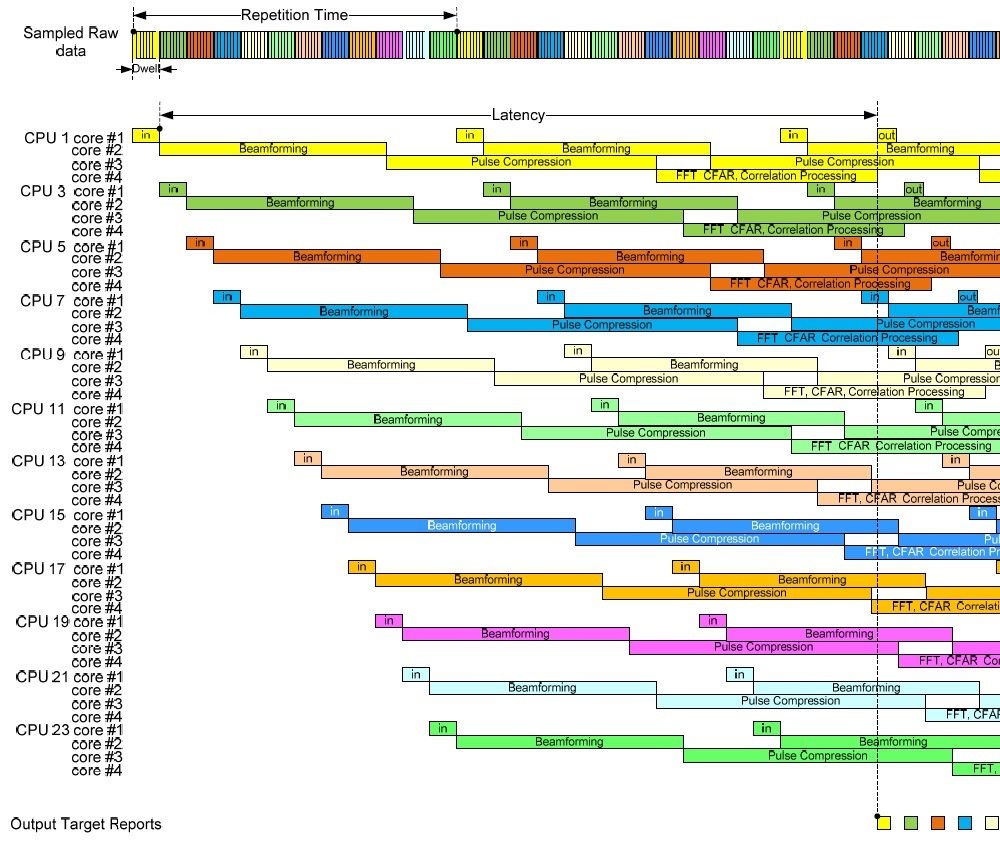
\includegraphics[width=140mm]{figures/aa_scheme1}
	\caption{A/A Mode Processing}
	\label{fig:existing_analysis:aa_scheme1}
\end{figure}


%%%%%%%%%%%%%%%%%%%%%%%%%
%%%%%  SSUB-SECTION   %%%
%%%%%%%%%%%%%%%%%%%%%%%%%
\subsubsection{Scheduling Scheme}
\label{sss:scheme1:aa:sched_blocks}
Scheduling functional blocks in the IMA processor architecture is shown in Figure \ref{fig:existing_analysis:aa_scheme1}. As discussed earlier, only odd numbered CPUs (CPU1,3,5...23) take part in processing A/A Mode algorithm.\\[0.3cm]
\textsl{Core\#1} receives incoming data from the Ethernet and stores them into Core\#1's buffer memory in SDRAM. Then the data is copied to Core\#2's buffer memory.\\[0.2cm]
%%%%%%
\textsl{Core\#2} transfers the data from its buffer memory to storage memory to L2 cache and then performs Beamforming. The results of the processing are stored back to the core\#3's buffer memory in SDRAM.\\[0.2cm]
%%%%%
\textsl{Core\#3} reads the data from its SDRAM partition and performs Pulse Compression. The results of the processing are stored back to the SDRAM.\\[0.2cm]
%%%%%%
\textsl{Core\#4} gets the data from its SDRAM partition and performs FFT, CFAR, Correlation Processing. The results of the processing are stored back to the SDRAM.

%%%%%%%%%%%%%%%%%%%%%%%%%
%%%%%  SSUB-SECTION   %%%
%%%%%%%%%%%%%%%%%%%%%%%%%
\subsubsection{CPU Utilization}
\label{sss:scheme1:aa:cpu_util}
CPU utilization is the ratio of processing time to the available time. The worst case available time of a CPU is the time span between receiving two shortest Dwells by the CPU, calculated as 12x shortest Dwell time. The results reported here are rounded to two decimal places. The burst configurations and processor parameters are stated in the Chapter \ref{ss:aa_mode:radar_char}. Calculations for the first burst of the look direction-1 is explained in Appendix \ref{app:ba:calc:scheme1}. 

%9.83%	11.68%	13.83%	16.32%	19.16%
\begin{figure}
\begin{minipage}{\linewidth}
	\begin{minipage}{0.45\linewidth}
		\resizebox {7cm} {!} {
			\begin{tikzpicture}{width=7cm}
			\begin{axis}[
				x tick label style={/pgf/number format/1000 sep=},
				ylabel=Core\#1 Utilization in \%,
				xlabel=Look Direction,
				enlargelimits=0.05,
				legend style={at={(0.5,-0.1)},
				anchor=north,legend columns=-1},
				ybar interval=0.3,
				ymin=0,ymax=100,
				]
			\addplot 
				coordinates {(1, 9.83) (2, 11.68) (3, 13.83) (4, 16.32) (5, 19.16) (6, 19.16)};
			\end{axis}
			\end{tikzpicture}
		}
      \end{minipage}
      \hspace{0.05\linewidth}
      \begin{minipage}{0.45\linewidth}
	 \resizebox {7cm} {!} {
		\begin{tikzpicture}{width=5cm}
		\begin{axis}[
			x tick label style={/pgf/number format/1000 sep=},
			ylabel=Core\#2 Utilization in \%,
			xlabel=Look Direction,
			enlargelimits=0.05,
			legend style={at={(0.5,-0.1)},
			anchor=north,legend columns=-1},
			ybar interval=0.3,
			ymin=0,ymax=100,
			]
		\addplot
			coordinates {(1, 12.48) (2, 14.82) (3, 17.56) (4, 20.7) (5, 24.32) (6, 19.16)};
		\end{axis}
		\end{tikzpicture}
		}
	\end{minipage}
\end{minipage}

\vspace*{2cm}
\begin{minipage}{\linewidth}
	\begin{minipage}{0.45\linewidth}
		\resizebox {7cm} {!} {
			\begin{tikzpicture}{width=7cm}
			\begin{axis}[
				x tick label style={/pgf/number format/1000 sep=},
				ylabel=Core\#3 Utilization in \%,
				xlabel=Look Direction,
				enlargelimits=0.05,
				legend style={at={(0.5,-0.1)},
				anchor=north,legend columns=-1},
				ybar interval=0.3,
				ymin=0,ymax=100,
				]
			\addplot
				coordinates {(1, 33.68) (2, 37.22) (3, 44.1) (4, 52.02) (5, 65.65) (6, 19.16)};
			\end{axis}
			\end{tikzpicture}
		}
      \end{minipage}
      \hspace{0.05\linewidth}
      \begin{minipage}{0.45\linewidth}
	 \resizebox {7cm} {!} {
		\begin{tikzpicture}{width=5cm}
		\begin{axis}[
			x tick label style={/pgf/number format/1000 sep=},
			ylabel=Core\#4 Utilization in \%,
			xlabel=Look Direction,
			enlargelimits=0.05,
			legend style={at={(0.5,-0.1)},
			anchor=north,legend columns=-1},
			ybar interval=0.3,
			ymin=0,ymax=100,
			]
		\addplot
			coordinates {(1, 43.9) (2, 50.21) (3, 58.67) (4, 64.53) (5, 75.58) (6, 19.16)};
		\end{axis}
		\end{tikzpicture}
		}
	\end{minipage}
\end{minipage}
\caption{CPU Utilization}
\label{ext_ana:sch1:cpu_util}
\end{figure}

CPU utilization is shown in Figure \ref{ext_ana:sch1:cpu_util} for each Core. On every Core, Look Direction-5 contributes to the highest(worst-case) processing time. It is evident from the figure that the Core\#1 and Core\#2 are utilized less than 25\%, meaning that the I/O processing and Beam-forming are not computation intensive. On the other hand, Core\#3 and Core\#4 are utilized 65\% and 75\% of the available time, meaning that there is very less room to adapt future growth. Core\#3 and Core\#4 violates the Radar processor requirements in terms of CPU utilization.

%%%%%%%%%%%%%%%%%%%%%%%%%
%%%%%  SSUB-SECTION   %%%
%%%%%%%%%%%%%%%%%%%%%%%%%
\subsubsection{Processing Latency}
\label{sss:scheme1:latency}
Processing Latency is the time between reception of a Dwell and sending of processed result data. As listed in Table \ref{tbl:existing_analysis:aa_scheme1_latency}, processing latency between 333ms and 617ms is achieved depending on the Look Direction.  Derivation of Look Direction-1's processing latency is explained in Appendix \ref{app:sch1:proc_late}. Number of Dwells the Radar can transmit, while the processor is busy in performing computations of a first received Dwell, is given as \textsl{\#Dwells transmitted}. Higher the \textsl{\#Dwells transmitted} implies that higher the stagnation of received echoes, which decreases the Radar processors response time. According to the Radar processor requirements, \textsl{\#Dwells transmitted} should be less than 2.

Time required to process a complete Dwell relate to the look direction-1 is shown in Figure \ref{fig:mm:scheme1_latency_tot}.
\begin{figure}[h!]
	\centering
	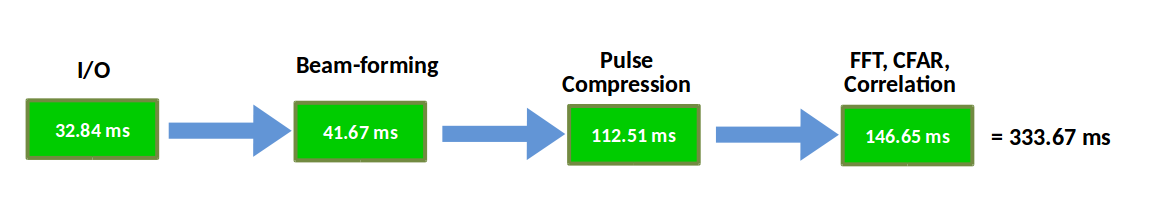
\includegraphics[width=145mm]{figures/scheme1_latency_tot}
	\caption{Dwell Processing time of Look Direction-1}
	\label{fig:mm:scheme1_latency_tot}
\end{figure}


\begin{table}[h!]
	\centering
	\begin{tabular}{|c|l|l|l|} 
	 \hline
	 \textbf{Look direction} & \textbf{Dwell time[ms]} & \textbf{Latency[ms]} & \textbf{\#Dwells transmitted} \\
	 \hline
	 1 & 27.84 & 333.67 & 11.99 \\ \hline
	 2 & 33.07 & 380.61 & 11.51 \\ \hline
	 3 & 39.17 & 448.16 & 11.44 \\ \hline
	 4 & 46.20 & 513.00 & 11.10 \\ \hline
	 5 & 54.26 & 617.05 & 11.37 \\ \hline
	\end{tabular}
	\caption{A/A Mode Processing Latency}
	\label{tbl:existing_analysis:aa_scheme1_latency}
\end{table}

%%%%%%%%%%%%%%%%%%%%%%%%%
%%%%%  SSUB-SECTION   %%%
%%%%%%%%%%%%%%%%%%%%%%%%%
\subsubsection{Memory Utilization}
\label{sec:scheme1:mem_util}
Each CPU has 4GiB of externally connected SDRAM. It is assumed that 3GiB are allocated for OS, storing executable code, etc. 1GiB are available for the actual data processing. Input and output data size for the cores and calculation of the memory requirement are shown Appendix \ref{app:sch1:mem_util}. According to the estimation, 7\% of the available capacity is sufficient for A/A Mode processing.

%%%%%%%%%%%%%%%%%%%%%%%%%
%%%%%  SSUB-SECTION   %%%
%%%%%%%%%%%%%%%%%%%%%%%%%
\subsubsection{Interface Utilization}
\label{sec:scheme1:aa_interface_util}
Interfaces are the data routing paths in the Radar processor. Nominal bandwidth of 100MiB/s data rate is assumed for the interfaces.  Peak interface utilization is calculated as 72\% of the available 100MiB/s. The calculations are listed in Appendix \ref{fig:existing_analysis:aa_scheme1_interface_util}.

\subsubsection{Summary}
The CPUs in the DGPM are physically separated for A/A Mode and A/G Mode; accordingly the results will not change if the Radar processor is performing both the modes simultaneously. Space partitioning has 12x Dwell latency, utilizing 7\% of the available memory, 72\% of the interface and the following CPU utilization factors. Scheme-1 scheduling technique violates the requirements of the Radar processor in terms of processing latency, hence it is not applicable for real-time processing.

\begin{table}[h!]
	\centering
	\begin{tabular}{|l|l|l|l|l|} 
	 \hline
	& \textbf{Core\#1} & \textbf{Core\#2} & \textbf{Core\#3} & \textbf{Core\#4} \\ \hline
	\textbf{Utilization} & 19.16\% & 24.32\% & 65.65\% & 75.58\% \\ \hline
	\end{tabular}
	\caption{CPU Utilization}
\end{table}

\clearpage
%%%%%%%%%%%%%%%%%%%%%%%%%%%%%%%%%%%%%
%%%%%%%%%%%%%%%%%%%%%%%%%%%%%%%%%%%%%
%%%%%%%%%%%%   SECTION   %%%%%%%%%%%%
%%%%%%%%%%%%%%%%%%%%%%%%%%%%%%%%%%%%%
%%%%%%%%%%%%%%%%%%%%%%%%%%%%%%%%%%%%%
\section{Scheme 2 - Time Partitioning}
\label{sec:scheme2}
Every CPU in the IMA processor architecture runs both the A/A mode and A/G mode application concurrently. CPU time and resources are shared for both the applications. Memory is partitioned for each mode to provide segregation. This analysis assumes
\begin{compactitem}
	\item All the four cores of a CPU can access SDRAM without interfering each other.
	\item L2 cache is statically partitioned at compile time, partition values are stated in Figure \ref{fig:existing_analysis:scheme2_partition_values}.
	\item Partition change time is 0.5ms. 
\end{compactitem} 

Figure \ref{fig:existing_analysis:scheme2_partition} shows the time partitioning of a CPU. Each application has to complete processing and suspend itself before the time slice expires. Otherwise a "deadline miss exception" is triggered.

\begin{figure}[h!]
	\centering
	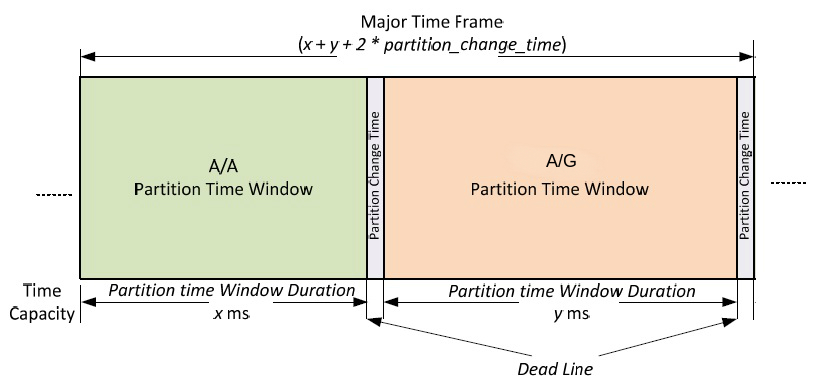
\includegraphics[height=55mm]{figures/scheme2_partition}
	\caption{Time Partition}
	\label{fig:existing_analysis:scheme2_partition}
\end{figure}

A/A data and A/G data are distributed by iCON1 to PSM1 and PSM2 respectively. Processed A/A data are transferred to iCON2 through PSM1. Partially processed A/G results from CPU1...CPU20 are transfered to CPU21...CPU24, where final A/G processing is carried out, followed by the results of the A/G processing are sent via PSM2 and iCON2 to a display.

\begin{figure}[h!]
	\centering
	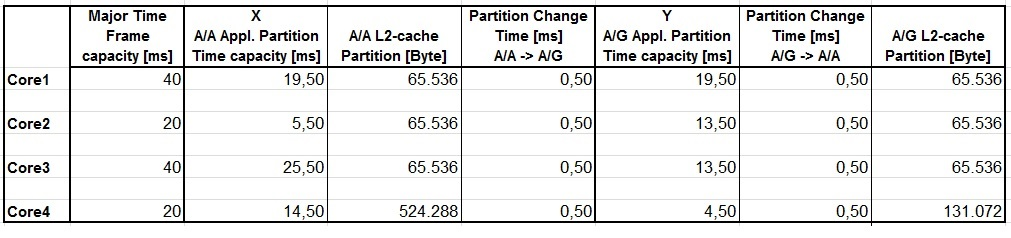
\includegraphics[width=150mm]{figures/scheme2_partition_values}
	\caption{Values for Time Partition}
	\label{fig:existing_analysis:scheme2_partition_values}
\end{figure}

\begin{figure}[h!]
	\centering
	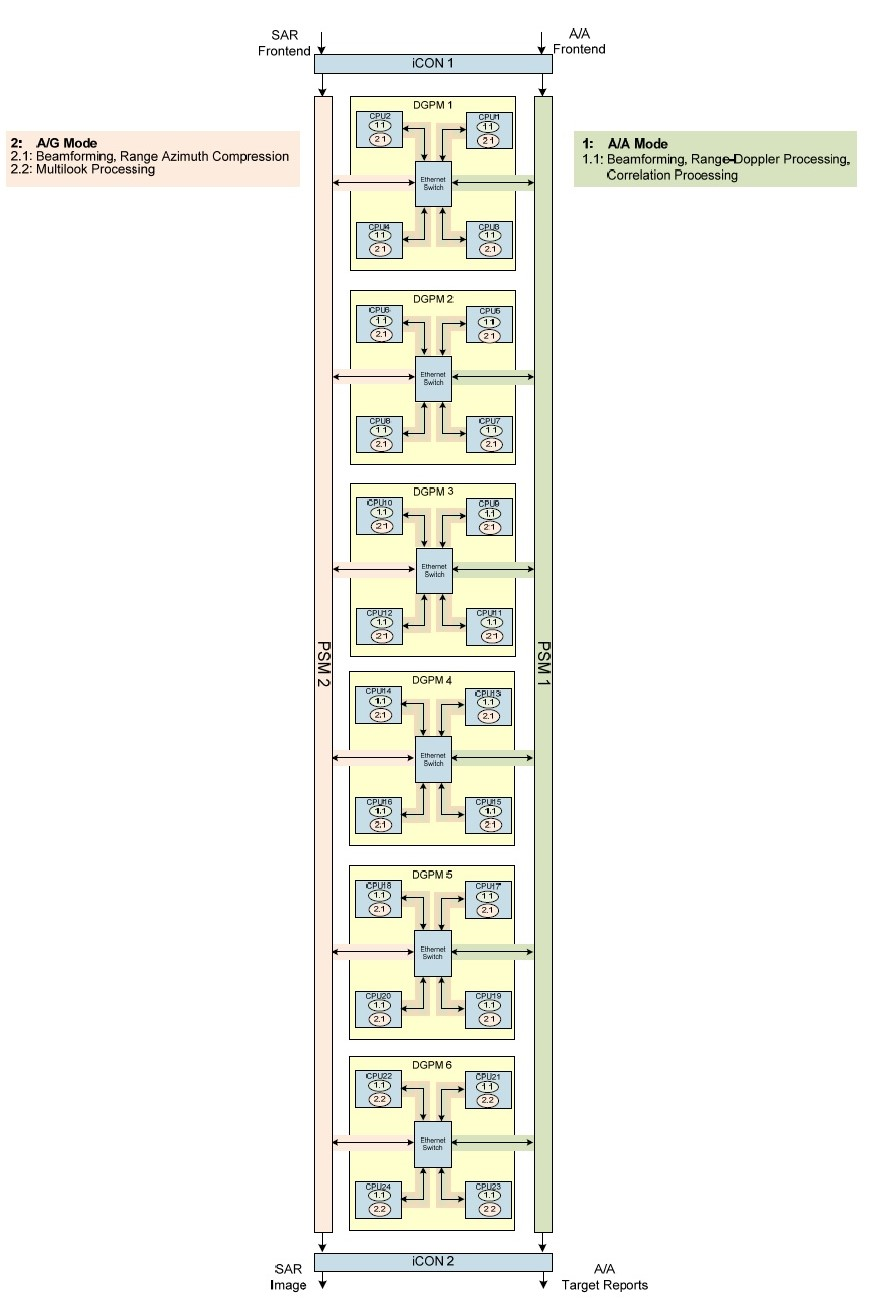
\includegraphics[width=160mm, height=220mm]{figures/scheme2_mode_mapping}
	\caption{Scheduling Scheme}
	\label{fig:existing_analysis:scheme2_mode_mapping}
\end{figure}
\clearpage

\subsection{A/A Mode Results}
\label{ss:scheme2:aa}
A/A Mode configuration is similar to the configuration discussed in Scheme-1, (see Chapter \ref{ss:scheme1:aa}) except that the data is distributed to 24 CPUs. There may be some additional time slots required to fit the processing into the allotted time slice. For instance, 33 time slots would provide sufficient time to complete a certain processing having 65536 loop counts. Therefore 1985 loops could be processed in each time slot. An additional 34$^{th}$ time slot would be required to execute the remaining 31 loops. This is called Time Slot Adjustment. Calculations are same as Scheme-1 and hence details of the cores processing time are not shown for simplicity.

\subsubsection{CPU Utilization}
\label{sss:scheme2:cpu_util}
Available time is 24x shortest Dwell time. Since the core is time sliced, effective available time is reduced by the factor of time slice and the processing latency is increased by the same factor. Table \ref{tbl:existing_analysis:aa_scheme2_cpu_util} lists the peak utilization values of each core.

\begin{table}[h!]
	\centering
	\begin{tabular}{|l|l|l|l|l|} 
	 \hline
	 & \textbf{Core\#1} & \textbf{Core\#2} & \textbf{Core\#3} & \textbf{Core\#4} \\ \hline
	 \textbf{Core Utilization} & 25\% & 53\% & 71\% & 63\% \\ \hline
	\end{tabular}
	\caption{CPU Utilization}
	\label{tbl:existing_analysis:aa_scheme2_cpu_util}
\end{table}

\subsubsection{Processing Latency}
\label{sss:scheme2:latency}
Processing latency is higher than Scheme-1 because a core gets approximately half of the available time for A/A Mode processing. Processing latency between 640ms and 1100ms is achieved depending on the look direction, which is also listed in Table \ref{tbl:existing_analysis:aa_scheme2_latency}.

Time required to process a complete Dwell relate to the look direction-1 is shown in Figure \ref{fig:mm:scheme2_latency_tot}.
\begin{figure}[h!]
	\centering
	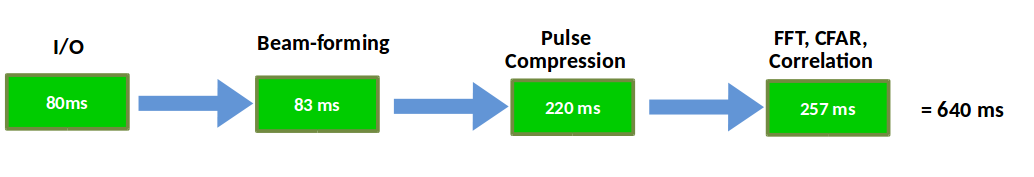
\includegraphics[width=145mm]{figures/scheme2_latency_tot}
	\caption{Dwell Processing time of Look Direction-1}
	\label{fig:mm:scheme2_latency_tot}
\end{figure}

\begin{table}[h!]
	\centering
	\begin{tabular}{|c|l|l|l|} 
	 \hline
	 \textbf{Look direction} & \textbf{Dwell time[ms]} & \textbf{Latency[ms]} & \textbf{\#Dwells transmitted} \\
	 \hline
	 1 & 27.84 & 640 & 22.99 \\ \hline
	 2 & 33.07 & 700 & 21.17 \\ \hline
	 3 & 39.17 & 820 & 20.93 \\ \hline
	 4 & 46.20 & 880.00 & 19.05 \\ \hline
	 5 & 54.26 & 1100 & 20.27 \\ \hline
	\end{tabular}
	\caption{A/A Mode Processing Latency}
	\label{tbl:existing_analysis:aa_scheme2_latency}
\end{table}
\FloatBarrier

\subsubsection{Memory Utilization}
\label{sss:scheme2:mem_util}
Each CPU has 4GiB of externally connected SDRAM. It is assumed that 3GiB are allocated for OS, storing executable code, etc, 1GiB are available for data processing. The peak memory utilization is calculated as 9\% of the available memory.

\subsubsection{Interface Utilization}
\label{sss:scheme2:interface_util}
Data distribution scheme is the extended version of Scheme-1, hence the peak interface utilization remains same as 72\%.

\subsection{Summary}
\label{sss:scheme2:sar_summary}
The Time Partition configuration has 23x Dwell time latency, utilizing 63\% of the CPU, 9\% of the memory and 72\% of the interface capability. Scheme-2 also failed to fulfil the Radar processor requirement. Neither of the baseline analysis scheme satisfies the real-time requirements. A Radar processor, having 23x Dwell time processing latency is not a good choice for airborne Radar processor. Next chapters explain optimal scheduling schemes to bring down the processing latency to an acceptable level.



\chapter{Test Bed and Design Decisions}
\label{chap:testbed}

%%%%%%%%%%%%%%%%%%%%%%%%%%%%%%%%%%%%%
%%%%%%%%%%%%%%%%%%%%%%%%%%%%%%%%%%%%%
%%%%%%%%%%%%   SECTION   %%%%%%%%%%%%
%%%%%%%%%%%%%%%%%%%%%%%%%%%%%%%%%%%%%
%%%%%%%%%%%%%%%%%%%%%%%%%%%%%%%%%%%%%
\section{Pros and Cons of the Baseline Analysis}
\label{sec:mm:pros_n_cons}
The contribution of this thesis starts with scrutinizing the Baseline Analysis. Upsides and downsides are investigated and their validity are verified.
\subsection{Pros}
\label{mm:pros}
Baseline analysis has considered every possible delicate detail to compute the worst case execution time. Upsides of the analysis are discussed here.

%\subsubsection{Cache Miss}
%Memory access time is different for different memory hierarchy levels. For instance, register memory can be accessed in one cycle, L1 cache in few cycles, L2 cache in 10 cycles and local DRAM needs approximately 100 cycles to be accessed by the CPU. To compute magnitude square root of 20 elements and store back the results to L1 cache, a core requires 280 cycles if the data are in L1 cache, 2140 cycles if the data are in SDRAM, assuming 4 cycles L1 access time and 10 cycle execution time per element. This kind of major variations are unfavourable for determinism. For safety critical systems the Worst Case Execution Time(WCET) needs to be analyzed and verified. The cache miss behaviour needs to be considered in the determination of the WCET. To achieve the worst case memory access times, it is assumed in the Existing Anlysis that a cache miss is produced for each memory access.

%One of the ways to calculate Worst Case Execution Time (WCET) is to assume cache miss always. This is a pessimistic approach as the cache hit ratio is not always 0\%. 

\subsubsection{CPU Utilization Balancing}
In time partition scheme, CPU utilization factors for A/A mode and A/G mode can be well balanced by configuring time slot period. For instance, in space partition scheme, Core\#4 is utilized 75\% in A/A mode processing and 25\% in A/G mode processing. This information gives a hint for time partitioning that A/A mode needs more time span than A/G mode in Core\#4. It is adopted in Scheme-2, allocating 14.5ms for A/A mode and 4.5ms for A/G Mode to balance the CPU utilization. Dynamic partition configuration can be considered in future to improve CPU utilization balancing.

\subsubsection{Memory Partitioning}
In time partition scheme, shared resources (L2 cache, Memory) are partitioned for A/A Mode and A/G mode to provide segregation. This isolation clearly defines the accessible address space for each core. Even if A/G mode processing of a core consumes huge memory space, A/A mode data of the core remains intact and will be useful during the next time slice. Another advantage of memory partitioning is, it allows utilization balancing among the memory resources.

\subsection{Cons}
\label{mm:cons}
\subsubsection{Context Switch Time}
Context switch time of 0.5ms is assumed for time partitioning. Every core does 2 context switches in 20ms. In time partition analysis (Scheme-2), at the end of 19.50ms all the four cores want to perform context switching. It is illustrated in Figure \ref{fig:mm:mm_cons1}. Since the SDRAM has only one port, it is possible for only one core to access the memory. Other cores have to wait till that time. 

\begin{figure}[h!]
	\centering
	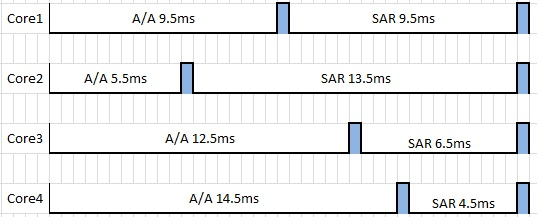
\includegraphics[width=120mm]{figures/mm_cons1}
	\caption{Time Partition of Scheme 3}
	\label{fig:mm:mm_cons1}
\end{figure}

Assuming the order of SDRAM access is Core\#1, Core\#2, Core\#3 and Core\#4. Core\#2 waits for Core\#1 to complete (0.5ms), Core\#3 waits for Core\#1,2 (0.5ms + 0.5ms), Core\#4 waits for Core\#1,2,3 (0.5ms + 0.5ms + 0.5ms). This overhead in waiting time sums up to 3ms. Though only one context switch is contending, during the course of run it will be a scenario where two context switches will contend for SDRAM because of its skewed timing behaviour. Worstcase waiting time for four cores is 
\begin{align*}
	& = \frac{4*T_{cs} \enspace + \enspace 2*T_{ow}}{T_{a}} \\[0.4cm]
	& = \frac{4*2*0.5ms \enspace + \enspace 2*3ms}{4*20ms} = 12.5\% \stepcounter{equation}\tag{\theequation} 
\end{align*}
\noindent
\textbf{Legend} \\
\tab $T_{cs}:$ Context-switch time \\
\tab $T_{ow}:$ Overhead in waiting time \\
\tab $T_{a}:$ Available time \\

In the worst case scenario, 12.5\% of the CPU time is spent only for context switching. This percentage is severe for a Radar processor. It degrades the application performance and much meaningful processing can be done during that time. \\

\textbf{\textsl{Verification:}} LMbench microbenchmark\cite{lmbench} is used to measure the context switch time of the ARM cores. LMbench is a free software suite of simple, portable benchmarks to compute various system performances including memory copy bandwidth, context switch latency, system call overhead, process creation latency, etc. Different sets of processes and data size are examined for the context switch time measurement. The LMbench suggests that the lowest recorded context switch time measurement is the more realistic one. So, lowest value of the 20 measurements are computed and listed in Table \ref{mm:ctxsw:lmbench}. 7.43$\mu$s in the table belongs to the context switch time measurement of two processes having 8KiB working data set each. The processes are scheduled according to the scheduling policy of the operating system. By monitoring the \verb|top| command, it is evident that the cores execute processes simultaneously, i.e. when four processes are involved in context switch, four cores are performing the execution.

\begin{table}[h!]
	\begin{tabularx}{\textwidth}{|X|X|X|X|X|}
		\hline
		\multirow{2}{*}{\textbf{Data Size [KiB]}} & \multicolumn{4}{c|}{\textbf{Context Switch Time[\boldmath$\mu$s]}} \\ \cline{2-5}
		& \textbf{2p} & \textbf{4p} & \textbf{8p} & \textbf{16p}  \\ \hline 
		8 & 7.43 & 9.09 & 12.76 & 13.58 \\ \hline
		16 & 8.22 & 16.35 & 19.31 & 20.87 \\ \hline
		32 & 9.57 & 18.48 & 23.68 & 29.13 \\ \hline
	\end{tabularx}
\caption{Measured Context Switch Time}
\label{mm:ctxsw:lmbench}
\end{table}

\begin{figure}[h!]
\centering
\begin{tikzpicture}
\begin{axis}[
	xlabel={No.of Processes},
	ylabel={Context Switch Time[$\mu$s]},
	legend pos=north west,
	ymajorgrids=true,
	grid style=dashed,
]
\addplot[color=red, mark=star,]
	coordinates {
		(2, 9.57) (4, 18.48) (8, 23.68) (16, 29.13)
	};

\addplot[color=black, mark=o,]
	coordinates {
		(2, 8.22) (4, 16.35) (8, 19.31) (16, 20.87)
	};
	
\addplot[color=blue, mark=square,]
	coordinates {
		(2, 7.43) (4, 9.09) (8, 12.76) (16, 13.58)
	};

	\legend{32K, 16K, 8K}
\end{axis}
\end{tikzpicture}
\caption{Comparison of Context Switch Time}
\label{mm:cntxt_switch_graph}
\end{figure}

From the above three sets of measurements, worst-case context switch time is 29.13$\mu$s corresponds to the 16 processes operating on 32KiB memory size. Also it reveals that the context switch time is proportional to the number of processes and data set size. On contrary to the assumption of 0.5ms context switch time and 12.5\% degradation in CPU utilization, measured worst-case context switch time is much lesser, therefore will not deteriorate the CPU utilization. So, no changes are made in the Baseline Analysis with respect to the context switch time.

\subsubsection{Clashing Data Streams}
In time partition scheme, assume that the Core\#1 of CPU1 is executing A/A Mode time slice. Now, A/G Mode data is routed to the same CPU by PSM2 as shown in Figure \ref{fig:mm:data_clash}. The core cannot accept the A/G Mode data as it is executing A/A time slice and the PSM have no idea of what the cores are up to or what to do with the data if the core is not accepting. This corner case is not clearly defined in the Baseline Analysis, as a result it leads to data loss if no countermeasure is provided.

\begin{figure}[h!]
	\centering
	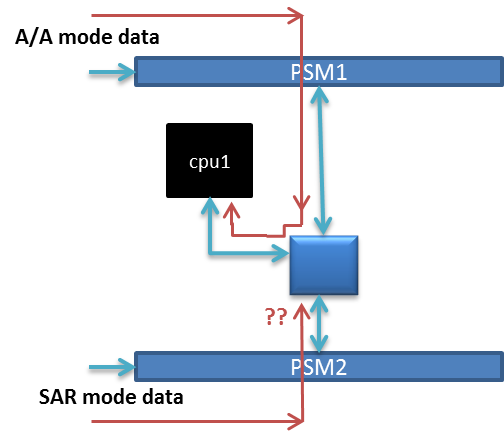
\includegraphics[width=80mm]{figures/data_clash}
	\caption{Clashing Data Streams}
	\label{fig:mm:data_clash}
\end{figure}

One of the ways to resolve this is to have a buffer in PSM to store the incoming data stream. If the core is not accepting the data, corresponding \verb|core_id| and \verb|cpu_id| shall be stored in the PSM along with the data. When the core is requesting data during next A/G Mode time slice, the PSM can transfer the stored data if the \verb|core_id| and \verb|cpu_id| matches. Since the incoming data stream is stored for one time slice period, it has to be counted for the processing latency calculation. The storing and restoring scheme ensures that the A/A data and A/G data will never be routed to the same CPU at the same time.

\subsubsection{Scalability}
\label{sss:mm:cons:scalability}
For time slot adjustment, it is cumbersome task to break the entire application into pieces such that each and every piece will fit in to one time slot. Whenever there is a change in time slot period, the entire application requires rework to suspend itself before the time slot expires. It implies that the time and cost of the application development and maintenance will increase. In addition, amendments are needed if the Radar configuration such as PRF set is changed.

\subsection{Other Comments}
\subsection{Measured Values of the Baseline Analysis}
\label{mm:cons:real_values}
The execution cycles of the functional blocks gives in the previous chapter (Table \ref{sec:ch2:benchmark_results}) were not the same when measured in a real hardware. The measured execution cycles are adapted in the Baseline Analysis and the results are presented here.

\subsubsection{Scheme-1}
\begin{table}[h!]
	\centering
	\begin{tabular}{|l|l|l|l|l|} 
	 \hline
	& \textbf{Core\#1} & \textbf{Core\#2} & \textbf{Core\#3} & \textbf{Core\#4} \\ \hline
	\textbf{Utilization} & 19.03\% & 46.20\% & 65.78\% & {\color{red} 108.07\%} \\ \hline
	\end{tabular}
	\caption{Measured CPU Utilization of Scheme-1, A/A Mode}
	\label{tbl:mm:scheme1_true_util}
\end{table}

\begin{table}[h!]
	\centering
	\begin{tabular}{|c|l|l|l|} 
	 \hline
	 \textbf{Look direction} & \textbf{Dwell time[ms]} & \textbf{Latency[ms]} & \textbf{\#Dwells transmitted} \\
	 \hline
	 1 & 27.84 & 416.40 & 14.96 \\ \hline
	 2 & 33.07 & 482.28 & 14.58 \\ \hline
	 3 & 39.17 & 574.52 & 14.67 \\ \hline
	 4 & 46.20 & 662.80 & 14.35 \\ \hline
	 5 & 54.26 & 798.62 & 14.72 \\ \hline
	\end{tabular}
	\caption{Measured Processing Latency of Scheme-1, A/A Mode}
	\label{tbl:mm:scheme1_true_latency}
\end{table}
Core\#4 of the A/A Mode processing CPUs in Scheme-1 required more than the available time to process one Burst of the input data. It leads to unfaithful result as it cannot cope up the incoming data stream.
\FloatBarrier

\subsubsection{Scheme-2}
\begin{table}[h!]
	\centering
	\begin{tabular}{|l|l|l|l|l|} 
	 \hline
	& \textbf{Core\#1} & \textbf{Core\#2} & \textbf{Core\#3} & \textbf{Core\#4} \\ \hline
	\textbf{Utilization} & 25.00\% & {\color{red} 103.33\%} & 71.43\% & 83.33\% \\ \hline
	\end{tabular}
	\caption{Measured CPU Utilization of Scheme-2, A/A Mode}
	\label{tbl:mm:scheme2_true_util}
\end{table}

\begin{table}[h!]
	\centering
	\begin{tabular}{|c|l|l|l|} 
	 \hline
	 \textbf{Look direction} & \textbf{Dwell time[ms]} & \textbf{Latency[ms]} & \textbf{\#Dwells transmitted} \\
	 \hline
	 1 & 27.84 & 860.00 & 30.89 \\ \hline
	 2 & 33.07 & 920.00 & 27.82 \\ \hline
	 3 & 39.17 & 1060.00 & 27.06 \\ \hline
	 4 & 46.20 & 1220.00 & 26.41 \\ \hline
	 5 & 54.26 & 1520.00 & 28.01 \\ \hline
	\end{tabular}
	\caption{Measured Processing Latency of Scheme-2, A/A Mode}
	\label{tbl:mm:scheme2_true_latency}
\end{table}
\FloatBarrier
Here, Core\#2 is utilized beyond its limits and the Dwell time latency reaches up to 30x Dwell time. Both the Schemes will not adhere to the real-time requirements.

%\clearpage
%%%%%%%%%%%%%%%%%%%%%%%%%%%%%%%%%%%%%
%%%%%%%%%%%%%%%%%%%%%%%%%%%%%%%%%%%%%
%%%%%%%%%%%%   SECTION   %%%%%%%%%%%%
%%%%%%%%%%%%%%%%%%%%%%%%%%%%%%%%%%%%%
%%%%%%%%%%%%%%%%%%%%%%%%%%%%%%%%%%%%%
\section{Test Procedure} 
\label{sec:mm:test_procedure}
Measurements of the Radar processor requirement factors such as Processing latency, Memory transfer bandwidth, Peak memory utilization and CPU utilization are performed as follows.

%%%%%%%%%%%%%%%%%%%%%%%%%
%%%%%   SUB-SECTION   %%%
%%%%%%%%%%%%%%%%%%%%%%%%%
\subsection{Processing Latency (Worst Case Execution time)}
\label{ss:mm:latency}
Proper way of measuring the worst case execution time includes the following steps:
\begin{compactitem} 
	\item All the cores are set to begin the execution simultaneously to produce maximum communication bandwidth.
	\item Cache data are invalidated before and after the measurements to ensure that the data is always fetched from memory.
\end{compactitem} 

\noindent
The below mentioned methods are followed to improve the determinism:
\begin{compactitem} 
	\item Every core executes a predefined thread.
	\item Radar application is given higher priority than other user space programs. \\
\end{compactitem} 

In worst case scenario, all the four cores of a CPU will execute the same functional block, generating maximum communication bandwidth, L2 cache contention and memory contention. To ensure that all the cores are executing the same functional block, a synchronization function is provided (Appendix \ref{app:code:wait_for_others}). A thread reaches this synchronization function waits until all the other threads to join, afterwards all the threads begin executing functional block simultaneously.

Invalidating cache data from user space is not allowed in ARM Cortex A9 processor. On the other hand, writing a program that copies huge junk of data from one memory location to other memory location seems to clear the cache contents. But, because of the complex caching strategies, it is not guaranteed that the entire cache data are removed, thus leaving major portion of the cache intact.\footnote{A discussion about this in ARM Connected Community forum can be found at \url{http://community.arm.com/thread/8799}} 

To overcome this, the Radar functional block sequences are executed for 1000 iterations to measure the maximum execution time. A graph is drawn displaying the measured execution times during this 1000 iterations. However, there are some unexpected spikes ranging five times higher than the average execution time, which occurs at sporadic intervals. The Nitrogen6X board is running \texttt{ssh, GUI, network-manager}, background measurement tasks and other OS services along with the functional block application. It can be reasoned that any of the other applications interrupts a running thread, causing it to be blocked for a while. So, the measurement is showing unrealistic values. The measured execution time of Comparison (\hyperlink{benchmarks}{CMPR256}) functional block with spike and the resulting execution time after removing the spike are shown in Figure \ref{fig:mm:chop_off}. Every core runs one instance of the CMPR256 functional block for 1000 iterations. So, four core runs four instances, totally counting 4000 iterations, listed in x-axis of the graph.

\begin{figure}[h!]
	\centering
	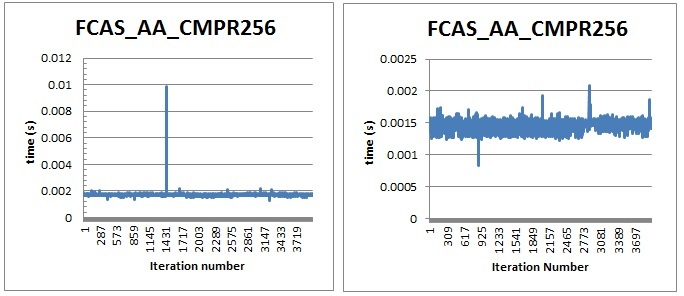
\includegraphics[width=150mm]{figures/chop_off}
	\caption{Before and After Spike Removal}
	\label{fig:mm:chop_off}
\end{figure}
A test run is made to study the effect of background tasks and services on the spikes. The background measurement tasks and services other than \verb|ssh, network-manager| are stopped. Now, only the minimal OS services are running. The Radar application is allowed to run in such less competitive environment. The result shows that the spikes are still occurring in few functional blocks, but the magnitude has reduced from 5x to 2x. As expected, execution time results of some short lived functional blocks do not have the spikes at all. It is concluded that the OS applications or services might have pre-empted the Radar application. Those spikes are removed from the graph and then the maximum execution time is computed. \vspace*{0.2cm}

To effectively utilize all the available four cores, four threads are spawned from main thread to carry out the parallel execution. Core affinity of each thread is set such a way that four threads are mapped to four cores (Appendix \ref{app:code:core_affinity}). For example, thread1 will run on Core\#1, thread2 on Core\#2, thread3 on Core\#3 and thread4 on Core\#4.\\
The Radar application is given higher priority than other user space tasks to give precedence. 

%%%%%%%%%%%%%%%%%%%%%%%%%
%%%%%   SUB-SECTION   %%%
%%%%%%%%%%%%%%%%%%%%%%%%%
\subsection{Memory Transfer Bandwidth}
\label{ss:mm:mem_bw}
Peak achievable memory bandwidth is measured by running threaded STREAM benchmark on Nitrogen6X board. Only STREAM benchmark is started by the user to guarantee that the measurement is not affected by other user applications. 

\lstset{ %
  backgroundcolor=\color{mildyellow},
  numbers=left,
  numberstyle=\tiny\color{mygray},
  frame=single,
  showspaces=false,
  showstringspaces=false,
  basicstyle=\ttfamily,
}

The measurement result of copying data from one memory location to another memory location is used for the  analysis. To measure the peak data transfer rate, the best result from 5 consecutive run is computed. As shown in Table \ref{tbl:mm:bw_no_load}, the iMX6Quad is capable of transferring \textbf{1048 MiB/s} when all the four cores are running in parallel.\\

\begin{table}[h!]
	\centering
	\begin{tabular}{|l|l|} 
	 \hline
	 \textbf{Function} & \textbf{Best Rate [MiB/s]}  \\
	 \hline
	 Copy & 1048.7 \\ \hline
	\end{tabular}
	\caption{Idle Memory Transfer Bandwidth}
	\label{tbl:mm:bw_no_load}
\end{table}

To compute the peak memory bandwidth of the Radar application, STREAM benchmark is allowed to run in background along with the Radar application. STREAM is given low priority to give precedence to the Radar application. When the Radar application is consuming maximum bandwidth, STREAM can only consume the minimum leftover bandwidth. Subtracting minimum recorded bandwidth from the peak memory bandwidth of the iMX6Quad (1048 MiB/s), gives peak memory bandwidth utilized by the Radar application.

%%%%%%%%%%%%%%%%%%%%%%%%%
%%%%%   SUB-SECTION   %%%
%%%%%%%%%%%%%%%%%%%%%%%%%
\subsection{Peak Memory Utilization}
\label{ss:mm:mem_util}
The percentage of the memory being used by a process can be extracted from \bverb|top| command. A bash script(Appendix \ref{app:code:mem_util}) is written to read memory utilization of the Radar application every 10 times a second. The recorded peak memory utilization is exported to an output file for further analysis. This script is also run in background at low priority.

%%%%%%%%%%%%%%%%%%%%%%%%%
%%%%%   SUB-SECTION   %%%
%%%%%%%%%%%%%%%%%%%%%%%%%
\subsection{CPU Utilization}
\label{ss:mm:cpu_load}
CPU utilization is the ratio of busy time to the total time. Busy time is the execution time on a particular CPU and total time is the time delay between two consecutive inputs to the same CPU. The CPU utilization says the percentage of utilization as well as the remaining buffer time for future growth. 50\% spare time is a healthy value for CPU utilization. This spare time can be used for health monitoring that reports hardware and software failures. By doing so, faults can be isolated and stopped from propagating.

\section{Performance Comparison of Single Core vs Four Cores}
\label{sec:mm:perf_comp}
A performance comparison study has been done on the Nitrogen6X board equipped with ARM Cortex A9 quad core processor running functional blocks of the Radar processing algorithm. In Figure \ref{fig:mm:1core_4core}, measurements of 1-thread, CMYACC means running CMYACC functional block on Core\#1 while keeping other cores in idle state. Likewise, measurements of 4-threads states that the CMYACC functional block is executed in all four cores simultaneously. The figure implies that the four core performance is not as good as single core performance. Bottleneck is imposed by the shared resources L2 cache and Memory. In-case more than one core wants to access a shared resource simultaneously, only one core is allowed to access them at a given time. Other cores have to wait until the shared resource is freed again. This increases worst-case execution time of the functional blocks when running on four cores. Although running four cores in parallel does increase the processing time, this thesis sticks to four core version to make use of all the execution resources.

\begin{figure}[h!]
	\centering
	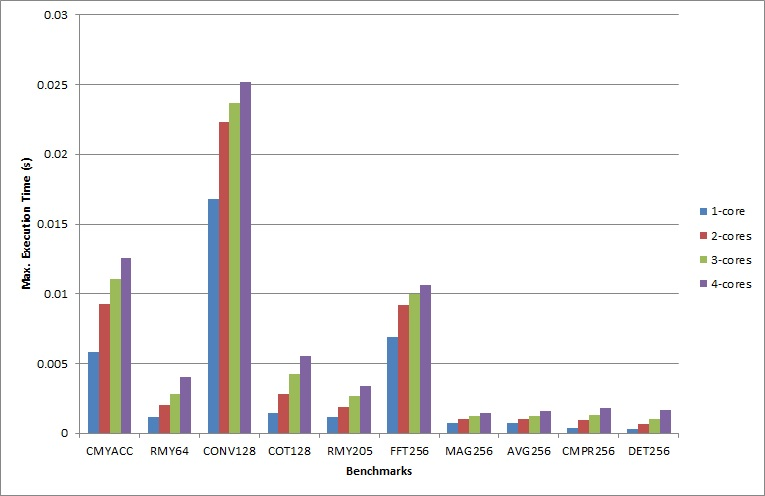
\includegraphics[width=140mm]{figures/1core_4core}
	\caption{Performance of Single Core vs Four Cores}
	\label{fig:mm:1core_4core}
\end{figure}


\clearpage
%%%%%%%%%%%%%%%%%%%%%%%%%%%%%%%%%%%%%
%%%%%%%%%%%%%%%%%%%%%%%%%%%%%%%%%%%%%
%%%%%%%%%%%%   SECTION   %%%%%%%%%%%%
%%%%%%%%%%%%%%%%%%%%%%%%%%%%%%%%%%%%%
%%%%%%%%%%%%%%%%%%%%%%%%%%%%%%%%%%%%%
\section{Design Decisions}
\label{mm:design_decisions}

\subsection{Parallel Execution}
Figure \ref{fig:mm:aa_serial_exe} illustrates the data distribution of Scheme-1 per CPU level. The diagram implies that the nature of execution is serial manner, in other words, it is equivalent to running the application on a single core processor. More CPUs and cores are used to improve the utilization factor, disregarding the processing latency. Thumb rule to reduce the processing latency is to process data independent portions of the application in parallel. 

\begin{figure}[h!]
	\centering
	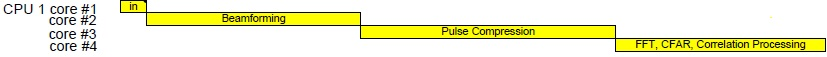
\includegraphics[width=160mm]{figures/aa_serial_exe}
	\caption{Serial Execution of A/A Mode Data in Baseline Analysis}
	\label{fig:mm:aa_serial_exe}
\end{figure}

\subsection{Balanced Utilization}
In all the schemes of the Baseline Analysis, Core\#1 of the A/A Mode CPU does only Input/Output operations, utilizing a smaller amount of the available CPU capability. Due to this, other cores of the CPU have to carry out rest of the processing, leaving them over utilized. This kind of skewed utilization figure pushes up the CPUs worst case utilization factor, so having well balanced utilization is a gesture of a healthy system. Core\#1 should also take part in processing the Radar application for utilization balancing as well as latency reduction. Static scheduling scheme shall be employed to balance the CPU utilization. \vspace*{0.2cm}

\subsection{Space Partition}
Evaluating the results of Time Partition scheme against Space Partition scheme, former one is considered to balance the CPU utilization by defining time slice periods. Down sides of the Time Partition scheme are:
\begin{compactitem} 
\item It magnifies latency by 2x compared to the Space Partition scheme.
\item As it requires breaking the entire application to fit into time slot, it is not scalable (see Chapter \ref{sss:mm:cons:scalability}).
\item Implementation needs more attention when it comes to memory partitioning.
\item Failure of one CPU will affect both the A/A mode and A/G mode processing.
\end{compactitem} 
\vspace*{0.2cm}
To sum up, Time Partition demands more effort and time to realise but producing no better result than Space Partitioning. So, this thesis decides to choose Space Partition as a base for further scheduling schemes.

\subsection{Dedicated Communication Channels}
Distributing the Radar raw data to different CPUs and gathering processed data increases total amount of communication. As depicted in Figure \ref{fig:mm:dedicated_channels}, dedicated channels for input, output between the DGPM and PSM shall be established in Space Partition configuration. It facilitates receiving incoming data stream and sending out processed data simultaneously without interference. The DGPM has 6 port Ethernet interface, of which 4 port shall be connected to 4 CPUs and remaining 2 ports shall act as dedicated input, output channels.

\begin{figure}[h!]
	\centering
	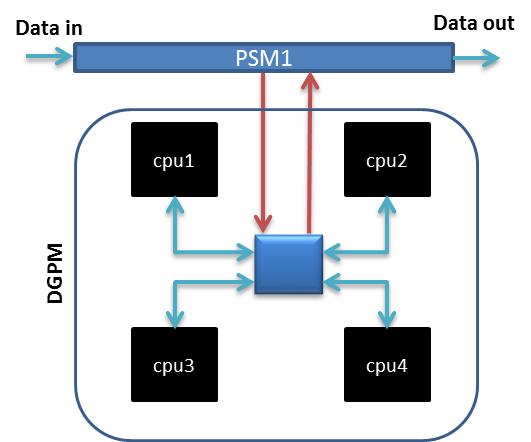
\includegraphics[width=60mm]{figures/dedicated_channels}
	\caption{Dedicated Communication Channels}
	\label{fig:mm:dedicated_channels}
\end{figure}

\subsection{Summary}
In a nut shell, this chapter has scrutinized the Baseline Analysis, discussed the techniques to measure the Radar processor requirement aspects and design choices that should be considered for optimal scheduling.


\chapter{Optimized Scheduling}
\label{chap:mode_mapping}

%%%%%%%%%%%%%%%%%%%%%%%%%%%%%%%%%%%%%
%%%%%%%%%%%%%%%%%%%%%%%%%%%%%%%%%%%%%
%%%%%%%%%%%%   SECTION   %%%%%%%%%%%%
%%%%%%%%%%%%%%%%%%%%%%%%%%%%%%%%%%%%%
%%%%%%%%%%%%%%%%%%%%%%%%%%%%%%%%%%%%%
\section{Scheme 3}
\label{sec:mm:scheme4}
According to the A/A Mode processing chain, only Correlation Processing is dependent on the results of the 8 bursts of a dwell. The burst processing chain except the correlation processing has no dependency and can therefore performed independently. The previous 7 bursts. Rest of the processing steps do not have any dependency, thus can be performed independently. The final Correlation Processing shall be computed serially. Space Partition configuration is adopted for Scheme-3 implementation.

\subsection{Hypothesis}
\textbf{\textsl{A Burst shall be processed as soon as a core receives it. This avoids unnecessary waiting time to receive a complete Dwell (8 Bursts) data.}}\\[0.2cm]
In case of the baseline analysis, as illustrated in Figure \ref{fig:mm:scheme4_data_distribution}, beam-forming of the first burst will start only after receiving a complete dwell. Though the first burst is ready for Beam-forming, redundant time is spent in waiting for the complete dwell data. This applies to the Pulse Compression, FFT, and CFAR processing also.

Scheme-3 exploits the fact that every burst can be processed independently until the Thresholding and Detection stage. Every burst is sent to an individual core to process them conveniently as soon as they are received. This saves waiting time during Data receive period, Beam-forming, Pulse compression, FFT and CFAR processing. Nothing has changed in terms of Correlation Processing, hence it will not contribute to the latency reduction.

\subsection{Scheduling Scheme}
As shown in Figure \ref{fig:mm:scheme4_aa_mode_mapping}, CPU1...6 are allocated for burst processing and CPU7 executes four instances of Correlation Processing in four cores, performing one instance per core. Burst processing comprises of Beam-forming, Pulse Compression, FFT and CFAR processing. A burst processing CPU gets four bursts and executes one instance of burst processing per core.

\begin{tabular}{rl}
	No.of cores for burst processing: & 6 x 4 = 24 \\
	No.of cores for correlation processing: & 1 x 4 = 4 \\
	Data distribution-burst processing: & One burst per core \\
	Data distribution-correlation processing: & One dwell per core \\
\end{tabular}
%\FloatBarrier 

\begin{figure}[h!]
	\centering
	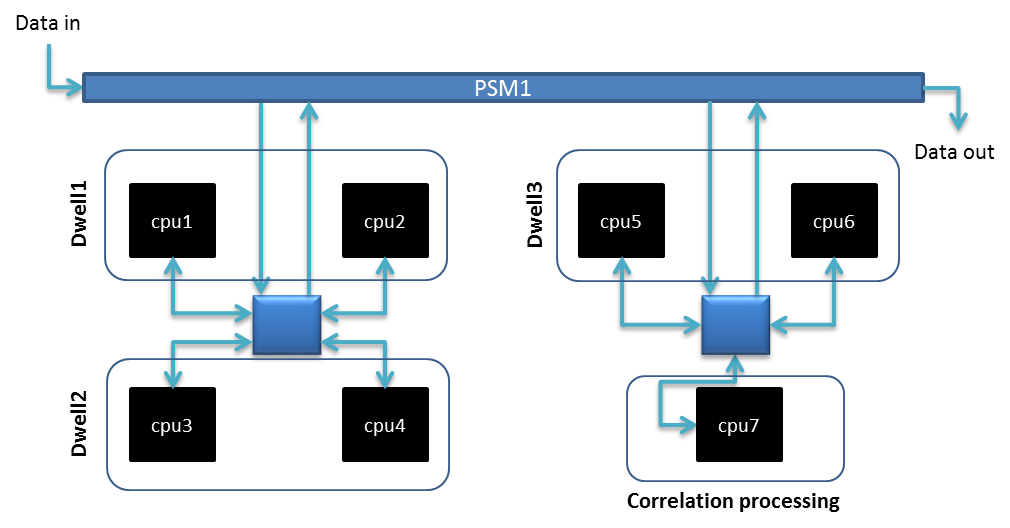
\includegraphics[width=140mm]{figures/scheme4_aa_mode_mapping}
	\caption{Scheduling Scheme}
	\label{fig:mm:scheme4_aa_mode_mapping}
\end{figure}

\vspace*{0.2cm}
\noindent
The received A/A mode raw data will be processed as follows

\begin{enumerate}
\item PSM1 routes each burst data to each core starting from core1 of CPU1 to core4 of CPU6 in round robin fashion.
\item Each core in the CPU1...6 performs burst processing followed by storing the results in SDRAM.
\item In a burst processing CPU, a core completing the processing steps last will transfer all the cores(Core\#1...\#4) results to the CPU7 for correlation processing. This avoids frequent communication between burst processing CPUs and correlation processing CPU. The data passed to the CPU7 is alarm list and their related information, which is smaller in size and assumed that it requires only 0.01ms to transfer.
\item Each core of the CPU7 waits for processed 8 burst data, and then performs Correlation Processing followed by sending out the target detections to PSM1.
\item PSM1 directs the results to tracking processor or display processor. Scheduling scheme is shown in Figure \ref{fig:mm:scheme4_data_distribution}.
\end{enumerate}

\begin{figure}[h!]
	\centering
	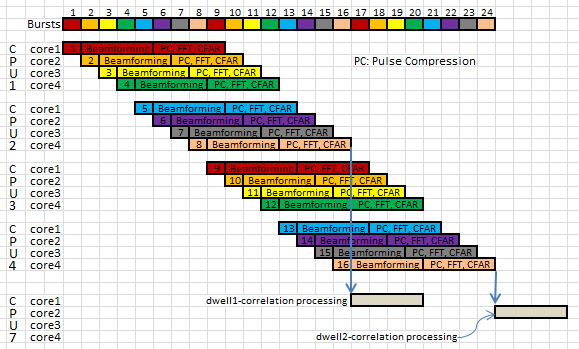
\includegraphics[width=140mm]{figures/scheme4_data_distribution.png}
	\caption{Scheduling Scheme}
	\label{fig:mm:scheme4_data_distribution}
\end{figure}

\begin{figure}[h!]
	\centering
	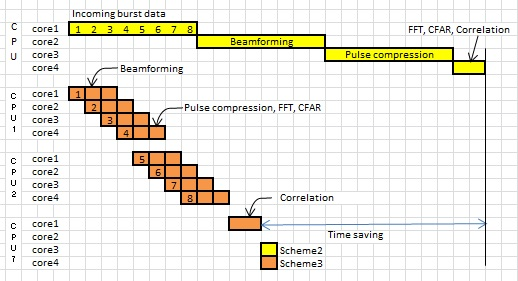
\includegraphics[]{figures/scheme4_comparison}
	\caption{Comparison of Scheduling Schemes}
	\label{fig:mm:scheme4_comparison}
\end{figure}

Another difference between Scheme-1 and Scheme-3 is the amount of data processed by a CPU. Scheme-1 performs 8 bursts processing whereas Scheme-3 performs 4 bursts processing per CPU. This decreases memory requirement and memory transfer bandwidth compared to the Scheme-1.

\subsection{Processing Latency}
\label{ss:mm:scheme4:latency}
Processing latency is measured on a real hardware clocked 1GHz and the results are scaled down to 800MHz. Data transfer time of 0.02ms is assumed between CPU1...6 and CPU7. Processing latency calculations of every core is shown in Appendix \ref{app:sch3:calc}. Figure \ref{fig:mm:scheme3_req_time} shows the latency components corresponds to PRF1, Look Direction-1 of one Burst.  Table \ref{fig:mm:scheme4_elapsed_time} summarizes the time required to process one burst until Thresholding and Detection stage.

\begin{figure}[h!]
	\centering
	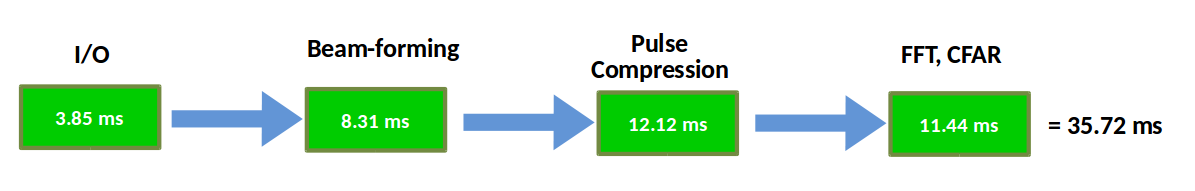
\includegraphics[width=145mm]{figures/scheme3_req_time}
	\caption{Burst Processing time for PRF1, Look Direction-1}
	\label{fig:mm:scheme3_req_time}
\end{figure}

The stated values in the table say that the look direction-1, PRF1 needs 35.72ms time to complete the execution from the moment a core starts receiving a burst. Elapsed wall clock time to process burst by burst is listed as \textsl{Time spent[ms]}. Example calculations for the look direction-1 are explained here with reference to the Figure \ref{fig:mm:scheme4_timeline_burst_proc}. A core waits for the pre-defined burst data to be received, i.e. a core processing PRF8 should wait till the PRF1...7 are distributed by the iCON. Burst receive time are derived from the Radar characteristics (see Chapter \ref{ss:aa_mode:radar_char}).

\begin{table}[h!]
	\centering
	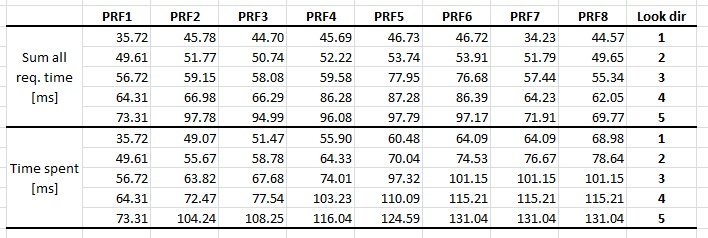
\includegraphics[width=140mm]{figures/scheme4_elapsed_time}
	\caption{Processing Time}
	\label{fig:mm:scheme4_elapsed_time}
\end{table}

\begin{figure}[h!]
	\centering
	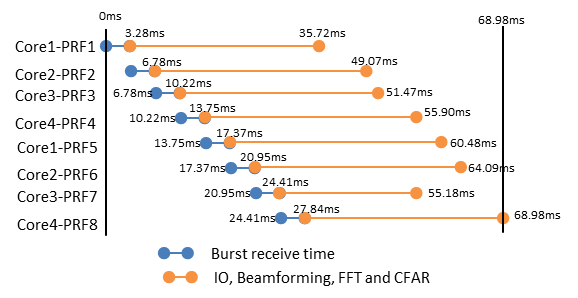
\includegraphics[width=130mm]{figures/scheme4_timeline_burst_proc}
	\caption{Elapsed Time Calculation}
	\label{fig:mm:scheme4_timeline_burst_proc}
\end{figure}

%\setlength{\belowdisplayskip}{2pt} \setlength{\belowdisplayshortskip}{2pt}
%\setlength{\abovedisplayskip}{0pt} \setlength{\abovedisplayshortskip}{0pt}
\begin{align*}
	T_{el} &= MAX((T_{pb} + T_{ex}), T_{el})\\
	PRF1 &= MAX((0 + 35.72), 0) = 35.72 \: ms\\
	PRF2 &= MAX((3.28 + 45.78), 35.72) = 49.07 \: ms \\	 
	PRF3 &= MAX((3.28 + 3.50 + 44.7),49.07) = 51.47 \: ms \\
		& \: \: . \\
		& \: \: . \\
		& \: \: . \\	
	PRF8 &= MAX((3.28 + 3.50 + 3.44 + 3.53 + 3.63 + 3.57 + 3.46 + 44.57), 64.09) \\
		&= 68.98 \: ms	\stepcounter{equation}\tag{\theequation}
\end{align*}
\noindent 
\textbf{Legend}\\
\tab $T_{el}:$ Elapsed time \\
\tab $T_{ex}:$ Execution time \\
\tab $T_{pb}:$ Previous burst receive time\\


Data transfer time of 0.02ms between burst processing CPUs and correlation processing CPU, and 0.2ms between correlation processing CPU and tracking/display processor is assumed.
\begin{align*}
	T_{l} &= T_{bp} + T_{dt} + T_{cp} + T_{tr}  \\
		&= 68.98 + 0.02 + 43.34 + 0.2 = 112.5 \: ms  \stepcounter{equation}\tag{\theequation}
\end{align*}
\noindent 
\textbf{Legend}\\
\tab $T_{l}:$ Processing latency \\
\tab $T_{bp}:$ Burst processing time \\
\tab $T_{dt}:$ Data transfer time from CPU1...6 to CPU7\\
\tab $T_{cp}:$ Correlation processing time \\
\tab $T_{tr}:$ Result transfer time from CPU7 to Tracking/Display processor \\

The processing latency between 112.52ms and 174.58ms are achieved depending on the look direction. Table \ref{tbl:mm:scheme4_latency} lists the processing latency of every look direction.
\begin{table}[h!]
	\centering
	\begin{tabular}{|c|l|l|l|} 
	 \hline
	 \textbf{Look direction} & \textbf{Dwell time[ms]} & \textbf{Latency[ms]} & \textbf{\#Dwells transmitted} \\
	 \hline
	 1 & 27.84 & 112.52 & 4.04 \\ \hline
	 2 & 33.07 & 122.18 & 3.69 \\ \hline
	 3 & 39.17 & 144.69 & 3.69 \\ \hline
	 4 & 46.20 & 158.75 & 3.44 \\ \hline
	 5 & 54.26 & 174.58 & 3.22 \\ \hline
	\end{tabular}
	\caption{Processing Latency}
	\label{tbl:mm:scheme4_latency}
\end{table}
\FloatBarrier

\subsection{CPU Utilization}
\label{ss:mm:scheme4:cpu_load}
\subsubsection{Burst Processing CPUs}
CPU utilization is the ratio of processing time to the available time. 6 CPUs are involved in A/A mode processing; meaning 24 cores are processing 24 burst (3 Dwell) data. Available time is 3x Dwell time. Utilization of each core per look direction is listed in Appendix \ref{fig:mm:scheme4_util}. Summarized utilization result is presented in Figure \ref{sch3:chrt:cpu_util}. From the figure, it can be seen that the maximum core utilization reaches up to 66\%.
\begin{figure}[h!]
\centering
\resizebox {10cm} {!} {
		\begin{tikzpicture}{}
		\begin{axis}[
			x tick label style={/pgf/number format/1000 sep=},
			ylabel=Max.Core Utilization in \%,
			xlabel=Look Direction,
			enlargelimits=0.05,
			legend style={at={(0.5,-0.1)},
			anchor=north,legend columns=-1},
			ybar interval=0.3,
			ymin=0,ymax=100,
			]
		\addplot
			coordinates {(1, 56) (2, 54) (3, 65) (4, 63) (5, 60) (6, 19.16)};
		\end{axis}
		\end{tikzpicture}
}
\caption{CPU Utilization - Burst Processing CPUs}
\label{sch3:chrt:cpu_util}
\end{figure}	
	
\subsubsection{Correlation Processing CPU}
\label{mm:SSS:scheme4:corr_cpu_util}
Correlation processing time values are listed in Appendix \ref{app:sch4:corr_cpu_util}. Processing time of one Dwell on a single core is given in Figure \ref{fig:mm:scheme4_corr_components}.

\begin{figure}[h!]
	\centering
	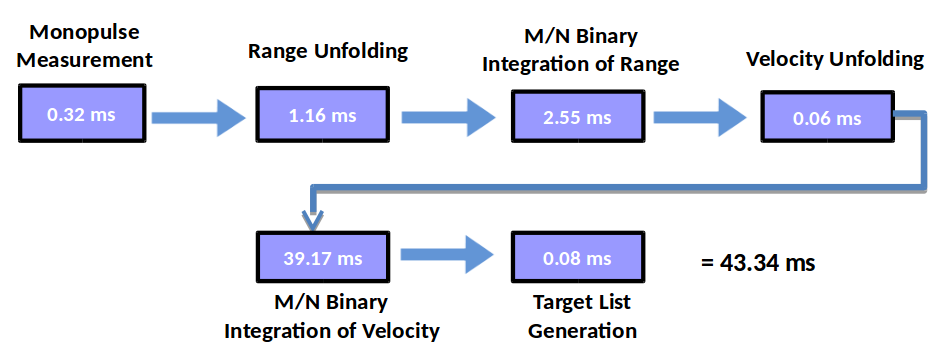
\includegraphics[width=120mm]{figures/scheme4_corr_components}
	\caption{Correlation Processing Time on a Single Core}
	\label{fig:mm:scheme4_corr_components}
\end{figure}

Every core of the correlation processing CPU is in idle state until it receives the results of 8 burst data from CPU1...6. Then it continues processing for 43.34ms before returning to idle state. Dwells are distributed to 4 cores of the CPU7 in round robin manner. Core\#1 of the CPU7 can start processing as soon as 8 bursts of a Dwell are received. 1ms delay is assumed between burst processing CPUs sending out the data and CPU7 starts processing. From the Table \ref{fig:mm:scheme4_elapsed_time}, look direction-1 needs 68.98ms to do burst processing. Until this time, Core\#1 of the CPU7 is in idle state. Correlation processing takes place for the next 43.34ms in Core\#1 followed by waiting for the next set Dwell5 data. Dwell5 will be supplied to the burst processing CPUs at 115.3ms (4 x 27.84ms) by the incoming data stream. Received Dwell5 data will be fed to CPU7 after 68.98ms (processing) + 1ms (transfer). From Figure \ref{sch3:chrt:corr_cpu_util}, peak utilization of the CPU7 is 39\%, belongs to the look direction-1. Utilization calculation for the look direction-1 is depicted in Figure \ref{fig:mm:scheme4_corr_cpu_util_pic}, and the utilization of Core\#1 is derived as follows.

\begin{align*}
	U_{1} &= \frac{T_{cp}}{ T_{cp} + T_{i}} = \frac{43.34}{43.34 + 69.98} = 38\% \\[0.4cm]
	T_{ndi} &= I_{d5} + T_{bp} \\
	&= 4 * 27.84 + 69.98 =181.3 \: ms\\
	T_{i} &= T_{ndi} - T_{ldo} \\
	&= 181.33 - (69.98 + 43.34) = 68.01 \: ms \\
	U_{5} &= \frac{43.34}{43.34 + 68.01} = 39\%  \stepcounter{equation}\tag{\theequation}
\end{align*}
\noindent 
\textbf{Legend}\\
\tab $U_{1}:$ Utilization at Dwell1 \\
\tab $T_{cp}:$ Correlation processing time \\
\tab $T_{i}:$ Idle time \\
\tab $T_{ndi}:$ Next Dwell in \\
\tab $T_{ldo}:$ Last Dwell out \\
\tab $T_{bp}:$ Burst processing time \\
\tab $I_{d5}:$ Dwell5 input at burst processing CPU 

\begin{figure}[h!]
	\centering
	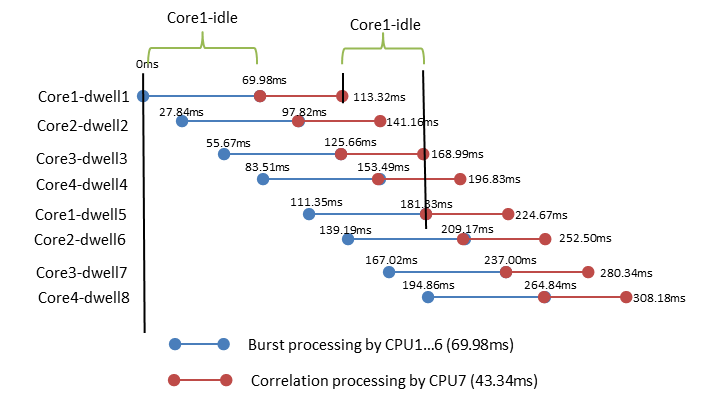
\includegraphics[width=160mm]{figures/scheme4_corr_timeline}
	\caption{Core\#1 - Idle Time, While Processing Look Direction-1 }
	\label{fig:mm:scheme4_corr_cpu_util_pic}
\end{figure}

\begin{figure}[h!]
\centering
\resizebox {10cm} {!} {
		\begin{tikzpicture}{}
		\begin{axis}[
			x tick label style={/pgf/number format/1000 sep=},
			ylabel=Max.Core Utilization in \%,
			xlabel=Look Direction,
			enlargelimits=0.05,
			legend style={at={(0.5,-0.1)},
			anchor=north,legend columns=-1},
			ybar interval=0.3,
			ymin=0,ymax=100,
			]
		\addplot
			coordinates {(1, 39) (2, 35) (3, 30) (4, 27) (5, 25) (6, 19.16)};
		\end{axis}
		\end{tikzpicture}
}
\caption{CPU Utilization - Burst Processing CPUs}
\label{sch3:chrt:corr_cpu_util}
\end{figure}

Utilization drops for ascending look direction, since look direction 5 has longest data receive time and processing time but maximum target detections are same for all the look directions. 
\FloatBarrier

\subsection{Memory Transfer Bandwidth}
\label{ss:mm:scheme4:bw_util}
Lowest recorded memory transfer bandwidth by running the STREAM benchmark as a background task is listed in Table \ref{tbl:mm:scheme4_mem_bw} 
Peak memory transfer bandwidth of the Radar application is measured as 39.4\% of the available 1048MiB/s.

\begin{table}[h!]
	\centering
	\begin{tabular}{|l|l|} 
	 \hline
	 \textbf{Function} & \textbf{Best Rate [MiB/s]} \\
	 \hline
	 Copy & 635.0 \\ \hline
	\end{tabular}
	\caption{Lowest Recorded Memory Transfer Bandwidth of the STREAM Benchmark}
	\label{tbl:mm:scheme4_mem_bw}
\end{table}

\begin{align*}
\label{aa:scheme4:mem_bw}
	BW_{p} &= BW_{i} - BW_{l} \\
	&= 1048 - 635 = 413 \: MiB/s \\
	&= \frac{413}{1048} = 39.4 \% \stepcounter{equation}\tag{\theequation} 
\end{align*}
\noindent 
\textbf{Legend}\\
\tab $BW_{p}:$ Peak bandwidth of the optimized scheme \\
\tab $BW_{i}:$ Idle bandwidth of the Nitrogen6X board \\
\tab $BW_{l}:$ Lowest recorded bandwidth \\

\subsection{Memory Utilization}
\label{ss:mm:scheme4:mem_util}
Peak memory utilization of the optimized scheme (Scheme-3) is measured as 0.9\% of the available 879MiB memory. Memory utilization is sampled 10 times a second until the A/A Mode sequence is running. Figure \ref{fig:mm:scheme4_mem_util} shows memory utilization footprint in a graphical view.

\begin{figure}[h!]
	\centering
	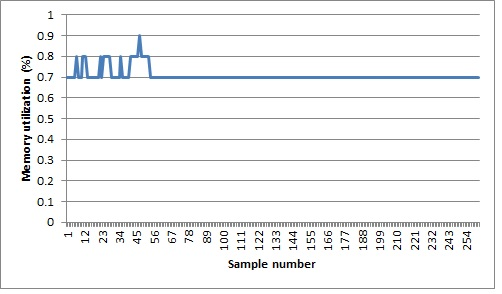
\includegraphics[width=100mm]{figures/scheme4_mem_util}
	\caption{Scheme-3, Memory Utilization Footprint}
	\label{fig:mm:scheme4_mem_util}
\end{figure}
\FloatBarrier

\subsection{Summary}
\label{ss:mm:scheme4:summary}
Scheme-3 has 4x Dwell time latency, 66\% CPU utilization, 39.4\% memory transfer bandwidth utilization and 1\% memory utilization. CPU utilization can be improved by adding more DGPMs. An IMA processor architecture can have upto 6 DGPMs comprising of 24 CPUs. Scheme-3 has utilized 28 cores of 7 CPUs, while rest of the 17 CPUs can be used for other purpose including A/G mode processing. A comparison of Scheme-1, Acceptable values and Scheme-3 is given below.

\begin{table}[h!]
	\centering
	\begin{tabular}{|l|l|l|l|} 
	 \hline
	 \textbf{Parameter} & \textbf{Scheme-1} & \textbf{Acceptable Values} & \textbf{Scheme-3}\\
	 \hline
	 Dwells transmitted &  14.96 & 2 & 4.04 \\ \hline
	 CPU utilization & 75.5\% & \textless 50\% & 66\% \\ \hline
	 Memory utilization & 7\% & \textless 50\%  & 1\% \\ \hline
	 Memory transfer bandwidth & NA & \textless 50\% & 41\%  \\ \hline
	\end{tabular}
	\caption{Comparison of Scheme-1 vs Acceptable Values vs Scheme-3}
	\label{tbl:mm:scheme4_comparison}
\end{table}

\clearpage
%%%%%%%%%%%%%%%%%%%%%%%%%%%%%%%%%%%%%
%%%%%%%%%%%%%%%%%%%%%%%%%%%%%%%%%%%%%
%%%%%%%%%%%%   SECTION   %%%%%%%%%%%%
%%%%%%%%%%%%%%%%%%%%%%%%%%%%%%%%%%%%%
%%%%%%%%%%%%%%%%%%%%%%%%%%%%%%%%%%%%%
\section{Scheme 4}
\label{sec:mm:scheme5}
Space Partition configuration is adopted for Scheme-4 implementation.
\subsection{Hypothesis}
\textsl{\textbf{Burst processing of each channel($S_{S},S_{G},S_{AZ},S_{EL}$) shall be performed in parallel as long as they are independent. This eliminates waiting time while processing other channel data. }}
\begin{compactitem}
\item Taking a closer look into the processing chain in Chapter \ref{sec:bg_related_work:proc_chain}, revels that a burst data has 4 channel processing namely Sum, Guard, Azimuth and Elevation.  These 4 channels do not have data dependency, allowing for parallel execution. In Scheme-3, Core\#1 does Beam-forming of one Burst serially, which comprises of computing Beam-forming for Sum channel, Azimuth channel and Elevation channel one after another. Scheme-4 proposes to perform them in parallel, leading to faster execution.
Data dependency diagram for A/A mode processing is shown in Figure \ref{fig:mm:scheme5_data_path}.

\begin{figure}[h!]
	\centering
	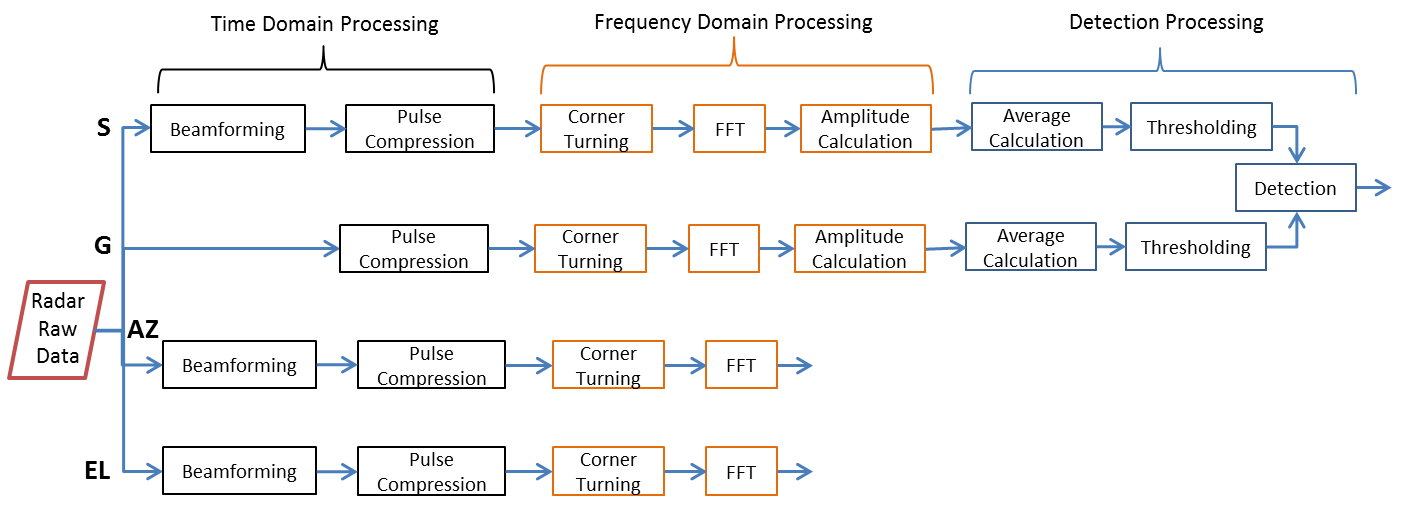
\includegraphics[width=160mm]{figures/scheme5_data_path}
	\caption{A/A Mode - Data Dependency of the Radar Application}
	\label{fig:mm:scheme5_data_path}
\end{figure}
Note: The data dependency diagram does not consider constant table values such as Sum channel beam-forming vector, Azimuth channel beam-forming vector, etc, as they are pre-calculated and available at any point of time.

\item Correlation processing shall be optimized to bring down the execution time.
\end{compactitem}

\subsection{Scheduling Scheme}
\label{ss:mm:scheme5:data_distribution}
Four channel processing are done by 4 cores of a CPU. CPU1...12 gets one burst each. CPU13 and CPU14 are allocated for correlation processing. 
PSM1 routs the Radar raw data to the respective DGPMs. Burst results are sent to PSM1 by the CPUs 1..12. PSM1 stores the burst result until 8 burst results are received. Then 8 burst results are sent to the cores of CPU13 and CPU14 in round robin manner. The DGPMs and PSM are arranged as shown in Figure \ref{fig:mm:scheme5_mode_mapping} and the data distribution is illustrated in Figure \ref{fig:mm:scheme5_data_distri}.

\begin{figure}[h!]
	\centering
	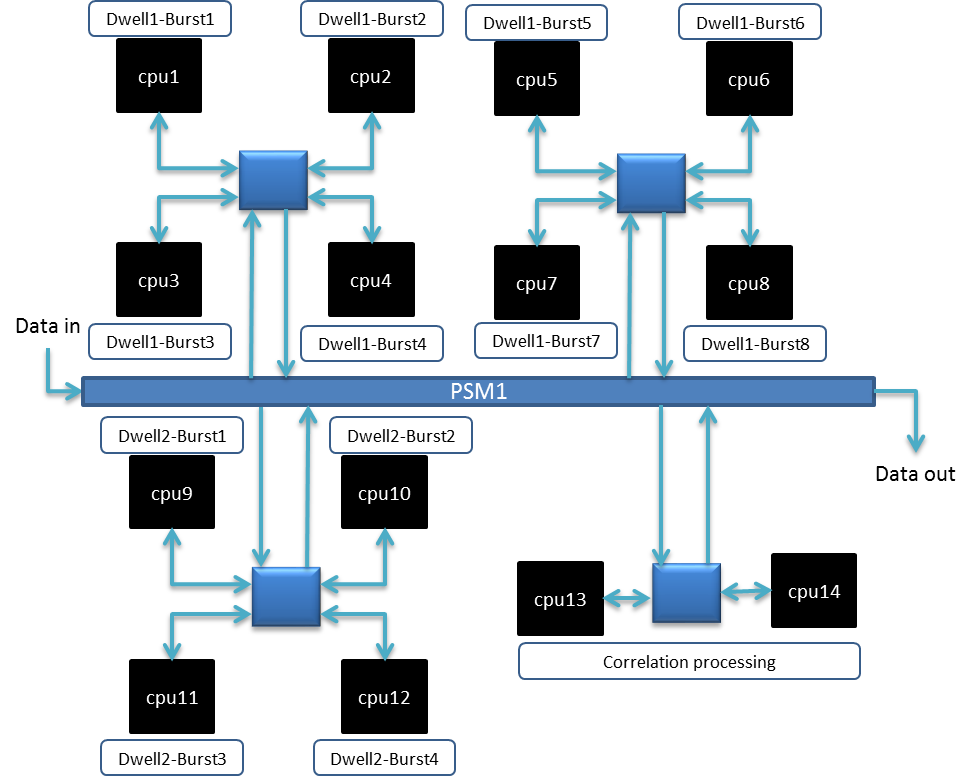
\includegraphics[width=130mm]{figures/scheme5_mode_mapping}
	\caption{Scheduling Scheme}
	\label{fig:mm:scheme5_mode_mapping}
\end{figure}

\begin{figure}[h!]
	\centering
	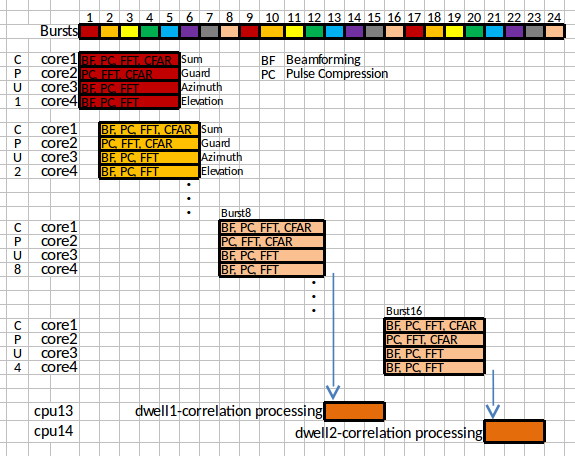
\includegraphics[width=130mm]{figures/scheme5_data_distri}
	\caption{Scheduling Scheme}
	\label{fig:mm:scheme5_data_distri}
\end{figure}

\begin{figure}[h!]
	\centering
	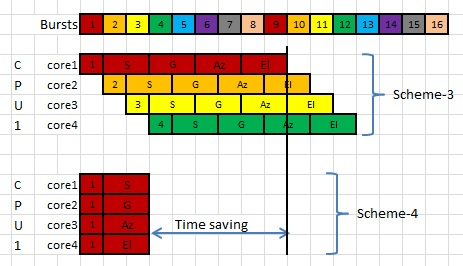
\includegraphics[width=95mm]{figures/scheme5_time_saving}
	\caption{Scheme-3 vs Scheme-4}
	\label{fig:mm:scheme5_time_saving}
\end{figure}

In terms of burst processing, every CPU in Scheme-3 performs computation on 4 burst data, whereas a CPU in Scheme-4 does computations on one burst. Single burst is placed in the shared memory, so that all the four cores can access them. CPU1 gets the first burst. Core1 of the CPU1 performs Beamforming, Pulse Compression, FFT and CFAR processing of Sum channel on the burst data. Rest of the three cores repeat the same for Guard channel, Azimuth and Elevation channel processing simultaneously. It results in approximately 4x reduced memory requirement than Scheme-3. A comparison of Scheme-3 and Scheme-4 is shown in Figure \ref{fig:mm:scheme5_time_saving}.
\FloatBarrier

Correlation processing requires 43.34ms (see Chapter \ref{mm:SSS:scheme4:corr_cpu_util}) to process one Dwell data. Dwell time of the look direction-1 is 27.84ms. Correlation processing itself consumes 1.5x Dwell transmission time. Best result cannot be achieved without optimizing the correlation processing. Pictorial view of the Correlation processing execution time is shown in Figure \ref{fig:mm:corr_proc_pie}.

\begin{figure}[h!]
	\centering
	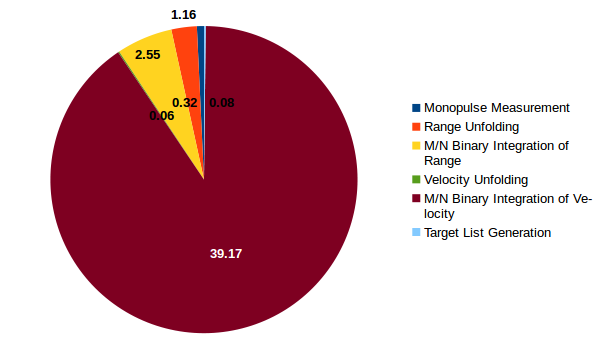
\includegraphics[width=120mm]{figures/corr_proc_pie}
	\caption{Correlation Processing - Processing Time in [ms]}
	\label{fig:mm:corr_proc_pie}
\end{figure}

According to the derivations of measurement time, M/N Binary Integration of Velocity(BIV) consumes 39.16ms of total 43.34ms. It is a good candidate for optimization. M/N BIV is implemented in \verb|C| according to the pseudo-code shown in Appendix \ref{app:sch4}, and the execution time is measured as 31.72ms when four instances are running on four cores. The loop iterations(Algorithm \ref{mm:biv:pseudo_code}, Line 3) of a single instance of M/N BIV are independent of the previous loop processing and next loop processing. They are broken into four sub-loops to run on four cores of a CPU in parallel. 4x speed-up is achieved for M/N Binary Integration of Velocity, reducing execution time from 31.72ms to 7.93ms. Any correlation processing CPU in Scheme-4 processes one dwell data, on contrary to the 4 dwell data in Scheme-3. Scheduling scheme and time saving are shown in Figure \ref{fig:mm:scheme5_corr_dd}, data dependency is shown in Figure \ref{fig:mm:scheme5_corr_data_path}.

\begin{figure}[h!]
	\centering
	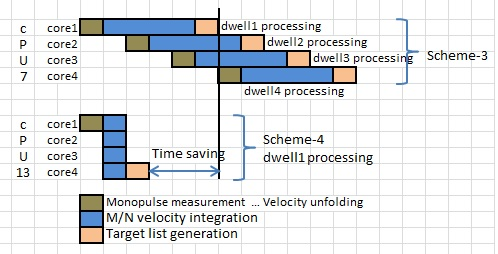
\includegraphics[width=95mm]{figures/scheme5_corr_dd}
	\caption{Comparison of Correlation Processing Schemes}
	\label{fig:mm:scheme5_corr_dd}
\end{figure}

\begin{figure}[h!]
	\centering
	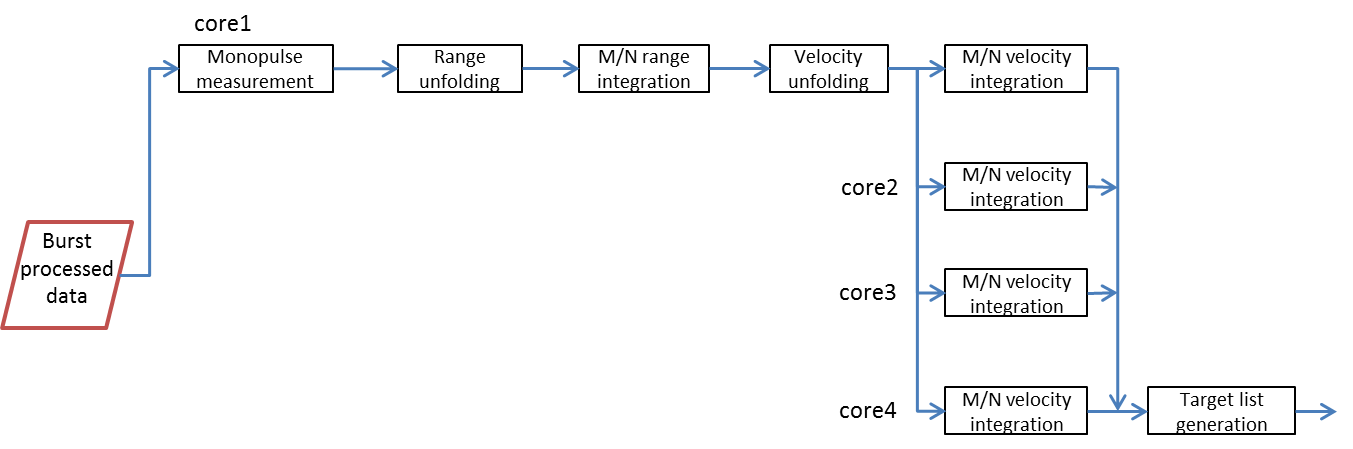
\includegraphics[width=140mm]{figures/scheme5_corr_data_path}
	\caption{Correlation Processing - Data Dependency and Scheduling Scheme}
	\label{fig:mm:scheme5_corr_data_path}
\end{figure}
At first, Core\#1 receives the dwell data for correlation processing, it does Monopulse measurement, Range unfolding, M/N range integration and Velocity unfolding serially. Afterwards, four threads are spawned to perform M/N BIV in parallel; each tread is allocated to a core. The thread completing M/N BIV last, will perform Target list generation followed by sending out the results to tracking/display processor via PSM1. Time delay of 0.02ms is assumed to spawn the threads and collect the results back. Resulting correlation processing time is calculated as follows. (Note: Execution time of the correlation processing steps can be seen in Figure \ref{fig:mm:scheme4_corr_calc})

\begin{align*}
\label{aa:scheme5:corr}
	T_{cp} &= T_{cp1} + T_{biv} + T_{tlg} +T_{ov} \\
	&= 4.09 + 7.93 + 0.02 + 0.02 = 12.06 \: ms \\ \stepcounter{equation}\tag{\theequation} 
\end{align*}
\noindent 
\textbf{Legend}\\
\tab $T_{cp1}:$ Monopulse measurement to Velocity unfolding processing time \\
\tab $T_{biv}:$ Time to process M/N BIV \\
\tab $T_{tlg}:$ Time to process Target list generation \\
\tab $T_{ov}:$ Overhead

\subsection{CPU Utilization}
\label{ss:mm:scheme5:cpu_load}
\subsubsection{Burst Processing CPUs}
Twelve CPUs are processing one burst each. Available time of a CPU is the time span between reception of two bursts to the CPU, which is 12x average burst time. Figure \ref{sch4:chrt:cpu_util} summarizes the CPU utilization for every look direction. Total time required to process one channel of a burst by a core is calculated as the sum of IO processing, Beam-forming, Pulse compression, FFT, CFAR, Thresholding, Detection and data copy time between SDRAM to the core. Detailed calculations can be found in appendix \ref{app:sch4_cpu_util}. As shown in the figure, it is implied that the peak CPU utilization reaches up to 50.8\%. Figure \ref{fig:mm:sch4_proc_time_chrt} shows the processing time of the Radar processing chain for Look direction-1, PRF1.

\begin{figure}[h!]
	\centering
	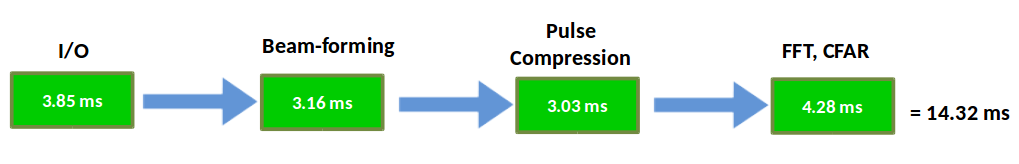
\includegraphics[width=140mm]{figures/sch4_proc_time_chrt}
	\caption{Burst Processing time for PRF1, Look Direction-1}
	\label{fig:mm:sch4_proc_time_chrt}
\end{figure}

\begin{figure}[h!]
\centering
\resizebox {10cm} {!} {
		\begin{tikzpicture}{}
		\begin{axis}[
			x tick label style={/pgf/number format/1000 sep=},
			ylabel=Max.Core Utilization in \%,
			xlabel=Look Direction,
			enlargelimits=0.05,
			legend style={at={(0.5,-0.1)},
			anchor=north,legend columns=-1},
			ybar interval=0.3,
			ymin=0,ymax=100,
			]
		\addplot
			coordinates {(1, 44.1) (2, 42.6) (3, 50.8) (4, 48.1) (5, 46.8) (6, 19.16)};
		\end{axis}
		\end{tikzpicture}
}
\caption{CPU Utilization - Burst Processing CPUs}
\label{sch4:chrt:cpu_util}
\end{figure}

\subsubsection{Correlation Processing CPUs} 
The data processed by the CPU1...12 are grouped as Dwells and sent to CPU13 and CPU14 alternatively. Correlation processing CPUs are in idle state until they receive a dwell data then performs computation for 12.06ms followed by waiting for next set of burst results from the next Dwell. Time delay of 0.02ms is assumed to transfer results from burst processing CPUs to correlation processing CPUs. Timeline diagram is illustrated in Figure \ref{fig:mm:scheme5_corr_timeline}. Utilization calculations for the look direction-1 are listed below. 

\begin{figure}[h!]
	\centering
	\includegraphics[]{figures/scheme5_corr_timeline}
	\caption{Look Direction-1, Utilization of the Correlation Processing CPU}
	\label{fig:mm:scheme5_corr_timeline}
\end{figure}

\begin{align*}
	U_{1} &= \frac{T_{cp}}{ T_{cp} + T_{i}} =  \frac{12.06}{12.06 + 42.54} = 22\% \\[0.4cm]
	T_{ndi} &= I_{d3} + T_{bp} \\
	&= 2 * 27.84 + 42.54 = 98.2 \: ms\\
	T_{i} &= T_{ndi} - T_{ldo} \\
	&= 98.2 - (12.06 + 42.54) = 43.6 \: ms \\
	U_{5} &= \frac{12.06}{12.06 + 43.6} = 22\%   \stepcounter{equation}\tag{\theequation}
\end{align*}

From the above calculation, it is seen that the peak utilization of the correlation processing CPU reaches upto 22\% when using two CPUs. Utilization of the Correlation processing CPUs for every look direction is given in Figure \ref{sch4:chrt:corr_cpu_util}.

\begin{figure}[h!]
\centering
\resizebox {10cm} {!} {
		\begin{tikzpicture}{}
		\begin{axis}[
			x tick label style={/pgf/number format/1000 sep=},
			ylabel=Max.Core Utilization in \%,
			xlabel=Look Direction,
			enlargelimits=0.05,
			legend style={at={(0.5,-0.1)},
			anchor=north,legend columns=-1},
			ybar interval=0.3,
			ymin=0,ymax=100,
			]
		\addplot
			coordinates {(1, 22) (2, 20) (3, 18) (4, 16) (5, 14) (6, 19.16)};
		\end{axis}
		\end{tikzpicture}
}
\caption{CPU Utilization - Correlation Processing CPUs}
\label{sch4:chrt:corr_cpu_util}
\end{figure}

\subsection{Processing Latency}
\label{ss:mm:scheme5:latency}
Processing latency between 54.79ms and 88.17ms is achieved depending on the look direction, which is the time required for burst processing and correlation processing. Maximum Dwell time latency(\textsl{\#Dwells transmitted}) is 1.97x Dwell time contributed by the look direction-1. The processing latencies of the look direction-1...5 are listed below. 

\begin{table}[h!]
	\centering
	\begin{tabular}{|c|l|l|l|} 
	 \hline
	 \textbf{Look direction} & \textbf{Dwell time[ms]} & \textbf{Latency[ms]} & \textbf{\#Dwells transmitted} \\
	 \hline
	 1 & 27.84 & 54.79 & 1.97 \\ \hline
	 2 & 33.07 & 61.43 & 1.86 \\ \hline
	 3 & 39.17 & 69.10 & 1.76 \\ \hline
	 4 & 46.20 & 77.98 & 1.69 \\ \hline
	 5 & 54.26 & 88.17 & 1.62 \\ \hline
	\end{tabular}
	\caption{Processing Latency}
	\label{tbl:mm:scheme5_latency}
\end{table}

\subsection{Memory Utilization}
\label{ss:mm:scheme5:mem_util}
Memory utilization of Scheme-4 is measured as 0.5\% of the available 879MiB memory. Memory requirement is reduced since, one CPU is working on one burst data, whereas in Scheme-3, one CPU gets 4 burst data. Memory utilization footprint of the Scheme-4 implementation is shown in Figure \ref{fig:mm:scheme4_mem_util}. Though the memory requirement is reduced by a factor of 4, memory utilization of the Scheme-4 is not reduced by the same figure. Since, the Scheme has FFTW library, spawning threads and other processing steps, that are required to run the application. They consume certain amount of memory regardless of the input data set.

\begin{figure}[h!]
	\centering
	\includegraphics[width=100mm]{figures/scheme5_mem_util}
	\caption{Memory Utilization Footprint}
	\label{fig:mm:scheme5_mem_util}
\end{figure}


\subsection{Memory Transfer Bandwidth}
\label{ss:mm:scheme5:bw_util}
Memory footprint is reduced compared to the Scheme-3, leading to a smaller amount of operating data set per core. Private L1 cache and shared L2 cache can hold large portion of the operating data set, reducing memory transfer between SDRAM to core and so reducing memory transfer bandwidth. The lowest recorded memory transfer bandwidth by running the STREAM benchmark as a background task is listed in Table \ref{tbl:mm:scheme5_mem_bw}. Peak memory transfer bandwidth of the Radar application is measured as 30.3\% of the available 1048MiB/s.

\begin{table}[h!]
	\centering
	\begin{tabular}{|l|l|} 
	 \hline
	 \textbf{Function} & \textbf{Best Rate [MiB/s]} \\
	 \hline
	 Copy & 729.9 \\ \hline
	\end{tabular}
	\caption{Lowest Recorded Memory Transfer Bandwidth of the STREAM Benchmark}
	\label{tbl:mm:scheme5_mem_bw}
\end{table}

\begin{align*}
\label{aa:scheme4:mem_bw}
	BW_{p} &= BW_{i} - BW_{l} \\
	&= 1048 - 729.9 =  318.1 \: MiB/s \\
	&= \frac{318.1}{1048} = 30.3 \% \stepcounter{equation}\tag{\theequation} 
\end{align*}

\subsection{Summary}
\label{ss:mm:scheme5:summary}

Processing latency of 1.92x Dwell time and peak CPU utilization of 50.8\% are healthy values for Air to Air Mode Radar processor. It leaves remaining 49\% of the CPU utilization to accommodate future development. In fact, 8 CPUs are sufficient to give same processing latency. More CPUs are used to improve the utilization. Figure \ref{fig:mm:scheme5_summary} shows the relationship between number of CPUs used and their utilization without affecting the latency values. Any combination of the CPU sets can be chosen to achieve desired CPU utilization. Selecting 10 CPUs for burst processing and 1 CPU for correlation processing will have peak CPU utilization of 61\% and 1.92x dwell latency, leaving rest of the 13 CPUs for A/G mode processing in an IMA processor architecture. A comparison of  Scheme-1, Acceptable values and Scheme-4 is listed in Table \ref{tbl:mm:scheme5_comparison}.

\begin{figure}[h!]
	\centering
	\includegraphics[width=90mm]{figures/scheme5_summary}
	\caption{Relationship Between Number of CPUs and Utilization}
	\label{fig:mm:scheme5_summary}
\end{figure}

\begin{table}[h!]
	\centering
	\begin{tabular}{|l|l|l|l|} 
	 \hline
	 \textbf{Parameter} & \textbf{Scheme-1} & \textbf{Acceptable Values} & \textbf{Scheme-4}\\
	 \hline
	 Dwell latency &  14.96 & 2 & 1.97 \\ \hline
	 CPU utilization & 75.5\% & \textless 50\% & 50.8\% \\ \hline
	 Memory Utilization & 7\% & \textless 50\%  & 0.5\% \\ \hline
	 Memory transfer bandwidth & NA & \textless 50\% & 30\%  \\ \hline
	\end{tabular}
	\caption{Comparison of Scheme-1 vs Acceptable Values vs Scheme-4}
	\label{tbl:mm:scheme5_comparison}
\end{table}

\section{Overview}
The Baseline Analysis has been observed to spot the latency contributors, bottlenecks and data dependencies. Upsides and downsides are evaluated to bring up the best scheduling scheme. Examined information have been supported in the design decisions of the scheduling scheme. Two new schemes are proposed to reduce the processing latency and they are validated via implementation. \vspace*{0.2cm}

Scheme-3 makes use of the fact that, the bursts in a Dwell can be processed independently until the Thresholding and Detection stage. This phenomenon skips waiting time in Beam-forming, Pulse compression, FFT, CFAR, Thresholding and Detection stage. This can be called as coarse grained parallelism. A dedicated processor is assigned for Correlation processing, without changing the execution method. Final outcome of the Scheme-3 is 4x Dwell time latency with 66\% CPU utilization. \vspace*{0.2cm}

Every burst data has large amount of fine grained parallelism. Four channel processing of a burst is done independently in Scheme-4, saving the waiting time for the other channel processing.  Correlation processing poses a bottleneck as the serial execution requires 1.5x Dwell time. Further, it is also parallelised and executed in dedicated CPUs. Deemed 2x Dwell time processing latency is achieved along with 50.8\% CPU utilization, provided 13 CPUs are performing computation. From the Table \ref{tbl:mm:scheme5_comparison} data, speed-up of the Scheme-4 compared to the best scheme(Scheme-1) in the Baseline Analysis is drawn as follows. \\

\begin{figure}[h!]
\centering
	\begin{tikzpicture}
		\begin{axis}[
			xlabel={Look direction},
			ylabel={Speedup},
			legend pos=north west,
			ymajorgrids=true,
			grid style=dashed,
		]
		\addplot[color=red, mark=star,]
			coordinates {
				(1, 7.6) (2, 7.85) (3, 8.31) (4, 8.50) (5, 9.06)
			};
		\legend{Scheme-4}
	\end{axis}
\end{tikzpicture}
\caption{Speed-up, Scheme-4 vs Scheme-1}
\label{mm:scheme5_speedup}
\end{figure}

The best results of the Baseline Analysis are 75.5\% peak CPU utilization and 15x Dwell time latency, provided 12 CPUs are executing the Radar processing algorithm. For the same utilization value, Scheme-4 needs only 9 CPU resources and delivers acceptable latency of 2x Dwell time.


\chapter{Future Scope and Conclusion}
\label{chap:conclusion}

%%%%%%%%%%%%%%%%%%%%%%%%%%%%%%%%%%%%%
%%%%%%%%%%%%%%%%%%%%%%%%%%%%%%%%%%%%%
%%%%%%%%%%%%   SECTION   %%%%%%%%%%%%
%%%%%%%%%%%%%%%%%%%%%%%%%%%%%%%%%%%%%
%%%%%%%%%%%%%%%%%%%%%%%%%%%%%%%%%%%%%
\section{Future Scope}
There are lot of space for fine tuning the application and extending this research work. Some of them are discussed below.

\subsection{Parallel Executable Modules}
Latency reduction is greatly influenced by the amount of parallelism available in the application. Among the A/A mode benchmarks, Convolution and FFT are the major latency contributors. Scheme-3 executes FFT for every channel (Sum, Guard, Azimuth and Elevation) in sequential order, whilst Scheme-4 performs channel computations in parallel. In any case, single instance of FFT library is executed in serial. Breaking the FFT and Convolution functional block into parallel executable modules will allow greater improvement of execution time. This enables more than one core performing FFT computation of one channel, resulting in speed-up factor of broken parallel modules. \vspace*{0.2cm}

Functional blocks like Complex Multiply Accumulate (CMYACC), Range Multiply (RMY), Magnitude (MAG), Area Average Calculation (AVG) and Comparison (CMPR) have high level of parallelism. Loop iterations in the above functional blocks can be split to run in parallel. Effective speed-up will be equal to number of parallel executable modules. Although breaking the application for parallel execution increases speed-up, it needs more computing entities to carry out the task and new scheduling schemes. This is a starting point of the optimization and requires further feasibility study.

\subsection{Architectural Features}
The \verb|FFTW| library might not have used special architecture features, since regardless of turning on the \verb|arm| specific compiler switches, it complained 
\begin{compactitem}
	\item[] \verb|not vectorized: not enough data-refs in basic block.|
	\item[] \verb|not vectorized: failed to find SLP opportunities in basic block.|
\end{compactitem}
So it is not optimized for ARM Cortex A9 platform. 128-bit advanced SIMD unit of the ARM Cortex A9 processor can perform four math operations of 32-bit data at the cost of one math operation. Exploiting such feature will reduce the latency of the computation heavy modules in single threaded as well as multi-threaded environment.

\subsection{Cache Performance}
The more the cache hit rate, the less the memory transfer between SDRAM and core. Fetching data from memory is relatively slow and expensive. Corner turning is implemented as generic row-column transpose form. The data access pattern row-column wise, makes frequent cache misses. Corner turning can be implemented by Cache-Oblivious Algorithm as explained in \textsl{Cache Oblivious Matrix Transposition:Simulation and Experiment} \cite{cot}, to improve data locality. This will reduce memory transfer bandwidth as well as execution time.  

In Scheme-4, the burst data size after beam-forming is 52KiB. A core having 32KiB private L1 cache can hold up to 61\% of the beamformed data. As an over approximation approach, 0\% cache hit rate is assumed for the analysis. This is not the case in real world. Cache hit rate prediction mechanism shall be employed to have more realistic results.

Effect of various L2-Cache size and Memory size can be performed to determine the optimal size for working set data. Another interesting cache profiling is \textsl{cache data utilization ratio}, it is the ratio of the amount of data fetched from memory to the amount of data used by the CPU before the data is evicted. Such measurements in L1 cache and L2 cache indicate whether changes in the algorithm will yield significant reduction in execution time.

\subsection{A/G Mode}
This thesis has only considered A/A Mode processing of the Radar processor. The techniques shall be extended to adopt A/G Mode processing. A Radar processor should be capable of performing A/A Mode and A/G Mode processing in real time.

%\clearpage
\section{Conclusion}
\label{sec:ch5:conclustion}
This thesis has presented the Airborne Radar processing chain on IMA processor architecture for safety critical systems and baseline  analysis. Inference from the baseline analysis is that the latency is far higher than the acceptable values. Data dependency is scrutinized to leverage parallelism in the application. Pseudo algorithm of the Radar processing chain is implemented and the latency is measured on a real hardware. Measurement tools for memory utilization and bandwidth utilization have been made. \vspace*{0.2cm}

Couple of optimization schemes have been implemented for Air to Air Mode processing. Based on the new scheduling schemes, the optimized scheme(Scheme-4) guarantees 7.5x speed-up than the baseline analysis with lesser number of resources. The achieved 2x Dwell time latency is healthy enough for the A/A Mode Radar processor. \vspace*{0.2cm}

This thesis concludes that the simplified A/A mode Radar processing can be done on the IMA processor architecture in real time. It saves space, weight and power requirements. To compare this in day to day life, eight Samsung Galaxy S-III mobiles are sufficient to deliver 2x Dwell time latency with 87\% CPU utilization!


%BIBLIOGRAPHY

\addcontentsline{toc}{chapter}{Bibliography}
\bibliographystyle{IEEEtran}
\fancyhead[RE]{\normalfont Bibliography}
\fancyhead[LO]{\normalfont Bibliography}
\bibliography{bibliography/IEEEabrv,bibliography/example}

%APPENDIX
\appendix
%%%%%%%%%%%%%%%%%%%%%%%%%%%%%%%%%%%%%%%%%%%%%%%%%%%%%%%%%%%%%%%%%%%%%%%%%%
%%%%%%%%%%%%   CAPTER   %%%%%%%%%%%%%%%%%%%%%%%%%%%%%%%%%%%%%%%%%%%%%%%%%%
%%%%%%%%%%%%%%%%%%%%%%%%%%%%%%%%%%%%%%%%%%%%%%%%%%%%%%%%%%%%%%%%%%%%%%%%%%
\chapter{Block Diagrams}
\label{chap:appendix}

\section{Nitrogen6X Development Kit}
\label{app:nitrogen6x}

\begin{figure}[h!]
	\centering
	\includegraphics[]{figures/nitrogen6x}
	\caption{Nitrogen6X Development Kit \cite{nitrogen6x}}
	\label{fig:app:nitrogen6x}
\end{figure}
\newpage

\section{iMX6Quad CPU}
\label{app:imx6q}

\begin{figure}[h!]
	\centering
	\includegraphics[width=160mm, height=110mm]{figures/imx6q}
	\caption{Internals of iMX6Quad CPU \cite{imx_spec}}
	\label{fig:app:imx6q}
\end{figure}

\cleardoublepage
\chapter{Description of the Benchmark Functions}
\label{description:benchmark}
\begin{longtable}{rp{120mm}}
	\hypertarget{benchmarks}{100CMYACC8:}& Multiply each element of a 100 x 8-element complex matrix with an 8-element complex vector and accumulate the 8 complex multiplication results to a single complex result, resulting in a 100 x 1-element complex matrix. \\[0.2cm]
	100RMY50: & Multiply each vector in a 100 x 50-element complex matrix with a 50-element float vector, resulting in a 100 x 50-element complex matrix.\\[0.2cm]
	100CONV64: & Perform fast convolution of a 100 x 64-element complex matrix: complex 64-pt FFT, followed by a multiplication with a 64-element float vector, followed by a 64-pt complex inverse FFT, resulting in a 100 x 64-element complex matrix. \\[0.2cm]
	150COT50: & Perform a corner turning of a 150 x 50 complex matrix into a 50 x 150 complex matrix incl. zero-padding of the elements from 150 to 256\\ [0.2cm]
	50MAG256: & Perform with a 50 x 256-element complex matrix a magnitude square-root calculation, resulting in a 50 x 256 float matrix. \\[0.2cm]
	64AVG100: & Calculate from a 64 x 100-element float matrix the average within a 5x5 area around the cell. Resulting in a 64 x 100-element float matrix. \\[0.2cm]
	64CMPR100: & Compare a 64 x 100-element float matrix with a float threshold. If  the threshold is exceeded, the corresponding element in a 64 x 100 boolean matrix shall be set to TRUE, otherwise set to FALSE. \\[0.2cm]
\end{longtable}
\cleardoublepage

%%%%%%%%%%%%%%%%%%%%%%%%%%%%%%%%%%%%%%%%%%%%%%%%%%%%%%%%%%%%%%%%%%%%%%%%%%
%%%%%%%%%%%%   CAPTER   %%%%%%%%%%%%%%%%%%%%%%%%%%%%%%%%%%%%%%%%%%%%%%%%%%
%%%%%%%%%%%%%%%%%%%%%%%%%%%%%%%%%%%%%%%%%%%%%%%%%%%%%%%%%%%%%%%%%%%%%%%%%%
\chapter{Code Snippets}
\label{app:code}

\section{set\_core\_affinity()}
\label{app:code:core_affinity}

\lstset{ %
  backgroundcolor=\color{mildyellow},
  basicstyle=\ttfamily\small,
  breakatwhitespace=false,
  breaklines=true,
  captionpos=b,
  commentstyle=\color{mygreen},
  keepspaces=true,
  keywordstyle=\color{blue},
  otherkeywords={cpu\_set\_t,pthread\_t},
  numbers=left,
  numberstyle=\tiny\color{mygray},
  frame=single,
  showspaces=false,
  showstringspaces=false,
  stringstyle=\color{mymauve},
  language=C
}

\begin{lstlisting}[caption=Set core affinity of calling thread]
int set_core_affinity(int core_id)
{
  int num_cores = sysconf(_SC_NPROCESSORS_ONLN);
  if (core_id < 0 || core_id >= num_cores)
    return CPU_AFFINITY_ERROR;

  cpu_set_t cpuset;
  CPU_ZERO(&cpuset);
  CPU_SET(core_id, &cpuset);

  pthread_t current_thread = pthread_self();
  if(pthread_setaffinity_np(current_thread, sizeof(cpu_set_t), &cpuset) != 0) 
    return CPU_AFFINITY_ERROR;

  return CPU_AFFINITY_OK;
}
\end{lstlisting}


\newpage
\section{wait\_for\_all\_threads()}
\label{app:code:wait_for_others}

\begin{lstlisting}[caption=Wait for other threads to join]
void wait_for_all_threads()
{
  while(awakenedThreads%NUM_THREADS != 0)
    sleep(0.001);

  pthread_mutex_lock(&mutex);
  readyThreads += 1;

  if(readyThreads == NUM_THREADS) {
    pthread_cond_broadcast(&cv_count);
  }

  while(readyThreads != NUM_THREADS)
    pthread_cond_wait(&cv_count, &mutex);

  ++awakenedThreads;
  if(awakenedThreads == NUM_THREADS){
    awakenedThreads = 0;
    readyThreads = 0;
  }

  pthread_mutex_unlock(&mutex);
}
\end{lstlisting}

\lstset{ %
  language=bash
}
\newpage
\section{mem\_util.sh}
\label{app:code:mem_util}
\begin{lstlisting}[caption=Peak Memory Utilization]
#!/bin/bash
ITER=1
PEAK_MEM=0
MEM_SIZE=`free -m | sed -n '2p'| awk '{print $2}'`
DATE_BEGIN=$(date +%Y-%m-%d" "%H:%M:%S)
OUTPUT_FILE="logs/peak_mem_util.csv"

echo "DATE BEGIN,${DATE_BEGIN}" > ${OUTPUT_FILE}

# Check for user input
if [ "$#" = "0" ]
then
# Read from file
PID=`cat logs/pid`
else
PID=$1
fi
echo "PID = ${PID}"

NAME=`cat /proc/${PID}/cmdline`
echo "Application name, ${NAME}" >> ${OUTPUT_FILE}
RES=`eval top -b -n ${ITER} | grep ${PID}`

while [ ! -z "$RES"  ]
do
#echo "res = ${RES}"
array=($RES)
PEAK_MEM=${array[9]}
echo "${PEAK_MEM}" >> ${OUTPUT_FILE}

#echo "Peak mem = ${PEAK_MEM}"
RES=`eval top -b -n ${ITER} | grep ${PID}`
sleep 0.1
done
\end{lstlisting}
\cleardoublepage

%%%%%%%%%%%%%%%%%%%%%%%%%%%%%%%%%%%%%%%%%%%%%%%%%%%%%%%%%%%%%%%%%%%%%%%%%%
%%%%%%%%%%%%   CAPTER   %%%%%%%%%%%%%%%%%%%%%%%%%%%%%%%%%%%%%%%%%%%%%%%%%%
%%%%%%%%%%%%%%%%%%%%%%%%%%%%%%%%%%%%%%%%%%%%%%%%%%%%%%%%%%%%%%%%%%%%%%%%%%
\chapter{Baseline Analysis Example Calculations}
\label{app:ba:calc:scheme1}

\section{Scheme-1}
\subsection{Utilization of Core\#1}
\begin{figure}[h!]
	\centering
	\includegraphics[width=150mm]{figures/aa_scheme1_cpu_util_1}
	\caption{Scheme-1, Core\#1 Utilization}
	\label{fig:existing_analysis:aa_scheme1_cpu_util1}
\end{figure}
\begin{align*}
	\label{aa:scheme1:core1:equ}
	Burst \enspace data \enspace input & = 64 pulses \enspace * \enspace 103 \frac{range gates}{pulse} \enspace * \enspace 9channel * 4\frac{byte}{sample}\\[0.3cm]
	& = 237,312 \enspace byte \\[0.3cm]
	Data \enspace receive \enspace time &= \frac{1}{19.5 \enspace * \enspace 10^{3} \enspace Hz} \enspace * \enspace 64 = 3.28 \enspace ms \\[0.3cm]
	Data \enspace copy \enspace time &= 237,312 byte \enspace * \enspace 2\frac{cycle}{byte} \enspace * \enspace 1.25\frac{ns}{cycle} = 0.59 \enspace ms \\[0.3cm]
	Required \enspace time &= 3.28ms + 0.59ms =  3.88ms\\[0.3cm]
	Available \enspace time &= 12 * min.dwelltime = 12*27.84ms = 334.05ms \stepcounter{equation}\tag{\theequation} 
\end{align*}

\subsection{Utilization of Core\#2}
\begin{figure}[h!]
	\centering
	\includegraphics[width=150mm]{figures/aa_scheme1_cpu_util_2}
	\caption{Scheme-1, Core\#2 Utilization}
	\label{fig:existing_analysis:aa_scheme1_cpu_util2}
\end{figure}
\begin{align*}
\label{aa:scheme1:core2:equ1}
	SDRAM \: to \: L2cache \: time &= 237,312 byte \, * \, 2.29\frac{cycle}{byte} \, * \, 1.25\frac{ns}{cycle} = 0.68 \, ms \\[0.3cm]
	Beamforming \: processing &= 3channel * 64pulses * 103 \frac{range gates}{pulse} * 79\frac{cycle}{8 element} \\[0.3cm] 
	&\qquad * 1.25\frac{ns}{cycle} * 1.3(OSoverhead) = 2.54ms\\[0.3cm]
	Beamformed \: data &= 4channel * 64pulses * 103 \frac{range gates}{pulse} *8\frac{byte}{sample} = 210,944byte \\[0.3cm]
	L2cache \: to \: SDRAM \: time &= 210,944 byte \, * \, 2.29\frac{cycle}{byte} \, * \, 1.25\frac{ns}{cycle} = 0.60 \, ms \\[0.3cm]
	Data \: copy \: time &= 210,944 byte \, * \, 2.2\frac{cycle}{byte} \, * \, 1.25\frac{ns}{cycle} = 0.53 \, ms \\[0.3cm]
	Required \: time &= 0.59ms + 0.68ms + 2.54ms + 0.60ms + 0.53ms = 4.94ms \stepcounter{equation}\tag{\theequation} 
\end{align*}


\subsection{Utilization of Core\#3}
\begin{figure}[h!]
	\centering
	\includegraphics[width=160mm]{figures/aa_scheme1_cpu_util_3}
	\caption{Scheme-1, Core\#3 Utilization}
	\label{fig:existing_analysis:aa_scheme1_cpu_util3}
\end{figure}
\begin{align*}
	\label{aa:scheme1:core3:equ}
	Pulse \: compression &= \bigg(\#channel * \#pulses (CONV128 +  \# \frac{range gates}{pulse} * RMY50)\bigg)\\[0.3cm]  
	& \quad * \# \: cycle \: time * OSoverhead\\[0.3cm] 
	&= (4 * 64 (24100 + 103 * 15)) * 1.25 * 1.3 = 10.67ms   \stepcounter{equation}\tag{\theequation} 
\end{align*}

\FloatBarrier
\subsection{Utilization of Core\#4}
\begin{align*}
	\label{aa:scheme1:core4:equ1}
	FDP \: time &= \bigg(4channel * (\#pulses * \# \frac{RG}{pulse} (COT50 + RMY50) + \# \frac{RG}{pulse} * FFT64) \\[0.3cm] 
	& \qquad + 2 * (\# \frac{range gates}{pulse} * 64 * MAG256)\bigg) * OSoverhead * cycle \, time \\[0.3cm]
	&= (4 * (64 * 103 (12 + 15) + 103 * 2550) + 2 * (103 * 64 * 20)) * 1.3 * 1.25ns \enspace \\[0.3cm]
	&= \enspace 3.29ms  \stepcounter{equation}\tag{\theequation} 
\end{align*}

\begin{figure}[h!]
	\centering
	\includegraphics[width=150mm]{figures/aa_scheme1_cpu_util_4}
	\caption{Scheme-1, Core\#4 Utilization}
	\label{fig:existing_analysis:aa_scheme1_cpu_util4}
\end{figure}

\begin{align*}
	\label{aa:scheme1:core4:equ2}
		Data \: size \: after \: FDP &=  64pulses * 103 \frac{range gates}{pulse} ( 2 * 8 + 2 * 4) = 158,208 \: byte\\[0.25cm] 
		L2cache \: to \: SDRAM &= 158,208 byte \, * \, 2.29\frac{cycle}{byte} \, * \, 1.25\frac{ns}{cycle} = 0.45 \, ms \\[0.25cm]
		Average \: Calculation &= 2channel * 103 \frac{range gates}{pulse} * 64(FFTsize) * 20(AVG100) * 2 \\
		&=  527,360 \: cycle \\[0.25cm]
		Comparison &= 2channel * 103 \frac{range gates}{pulse} * 64(FFTsize) * 7(CMPR100) \\
		&= 92,288 \: cycle \\[0.25cm]
		Detection &= 1channel * 103 \frac{range gates}{pulse} * 64(FFTsize) * 10(DET100) \\
		&= 65,920 \: cycle \\[0.25cm]
		Time \: required &= (Average \, calculation + Comparison + Detection) \\
		& \qquad * OSoverhead * cycle \, time \\[0.25cm]
		&= (527,360 + 92,288 + 65,920) * 1.3 * 1.25ns = 1.1ms \stepcounter{equation}\tag{\theequation} 
\end{align*}

\begin{align*}
	\label{aa:scheme1:core4:equ3}
		Monopulse \: Measurement &= 2channel * \#\frac{alarms}{burst} * \#\frac{cycle}{alarm} * OSoverhead * cycle \: time \\
		&= 2 * 32 * 500 * 1.3 * 1.25ns = 0.05 \: ms \\
		Range \: Unfolding &= \bigg(RG_{max} * \#\frac{cycle}{rangegate} + \# Unfoldings * \#\frac{alarms}{burst} * \#cycle\bigg) \\
		& \qquad *OSoverhead * cycle \: time \\
		&= (987 * 30 + 10 * 32 * 200) * 1.3 * 1.25ns = 0.15 \: ms \\
		M/N \: Range \: Integration &= \bigg(\#RangeGates * \#\frac{cycle}{rangegate} + \#Unfoldings * \#\frac{alarms}{burst} \\
		&\qquad * \#\frac{cycle}{alarm}\bigg) * OSoverhead *cycle \: time \\
		&= (988 * 40 + 32 * 10 * 500) * 1.3 * 1.25ns = 0.32 \: ms \\
		Velocity \: Unfolding &= \bigg(\#Unfoldings * \#\frac{alarms}{burst} * \#\frac{cycle}{alarm}\bigg) \\
		& \qquad * OSoverhead * \#cycle \: time \\
		&= (8 * 32 * 30) * 1.3 * 1.25ns = 0.01 \: ms \\
		M/N \: Velocity \: Integration &= \bigg(\#\frac{alarms}{burst} * \#Unfoldings^{2} * \#bursts * \#\frac{cycle}{alarm}\bigg) \\
		& \qquad * OSoverhead * cycle \: time \\
		&= (32 * 10^{2} * 8 * 80) * 1.3 * 1.25ns =  3.33 \: ms \\
		Target \: List \: Generation &= \bigg(\#targets * \#\frac{cycle}{target}\bigg) * OSoverhead * cycle \: time \\
		&= (16 * 100) * 1.3 * 1.25ns = 0.0026 \: ms \\
		Correlation \: Processing[ms] &= 0.05 + 0.15 + 0.32 + 0.01 + 3.33 + 0.0026 = 3.87 \: ms \\
		Required \: time[ms] &= 0.53 + 0.60 + 3.29 + 0.45 + 0.45 + 0.11 + 3.87 = 10.31 \: ms \stepcounter{equation}\tag{\theequation}
\end{align*}

\subsection{Processing Latency}
\label{app:sch1:proc_late}
\begin{align*}
	\label{aa:scheme1:latency}
		Processing \: latency &= IO + Beamforming + Pulse \: compression  + FFT,CFAR,Correlation \\
		&= 32.84 + 41.67 + 112.51 + 146.65 = 333.67 \: ms \\[0.3cm]
		\#Dwells \: transmitted &= \frac{processing \: latency}{dwell \: time} = \frac{333.67}{27.84} = 11.99 \stepcounter{equation}\tag{\theequation}
\end{align*}

\subsection{Memory Utilization}
\label{app:sch1:mem_util}
\begin{figure}[h!]
	\centering
	\includegraphics[width=160mm]{figures/aa_scheme1_mem_util}
	\caption{Scheme-1, Memory Utilization}
	\label{fig:existing_analysis:aa_scheme1_mem_util}
\end{figure}

\subsection{Interface Utilization}
\label{app:sch1:mem_util}
The DGPMs are identical, thus only one DGPM's utilization is listed here.
\begin{figure}[h!]
	\centering
	\includegraphics[width=160mm]{figures/aa_scheme1_interface_util}
	\caption{Scheme-1, Interface Utilization}
	\label{fig:existing_analysis:aa_scheme1_interface_util}
\end{figure}
\begin{align*}
	\label{equ:aa:scheme1:interface_util}
	iCON1 \: output \: to \: PSM1 &= \#\frac{byte}{sample} * \#channel * range \: gate * frequency \\
	&= 4 * 9 * 103 * 19.5kHz = 72.31 \: MB/s \\
	DGPM \: input \: from \: PSM &= \frac{data \: rate}{\#DGPMs} = \frac{72.31}{6} = 12.05 \: MB/s \\[0.3cm]
	CPU \: input &= \frac{DGPM \: data \: rate}{\#CPUs} = \frac{12.05}{2} = 6.02 \: MB/s \\[0.3cm]
	DGPM \: output \: to \: PSM &= \frac{data \: rate}{\#DGPMs} = \frac{0.31}{6} = 0.0526 \: MB/s \\[0.3cm]
	CPU \: output &= \frac{DGPM \: output}{\#CPUs} = \frac{0.0526}{2} = 0.026 \: MB/s \stepcounter{equation}\tag{\theequation}
\end{align*}

\chapter{Scheme-3 Calculations}
\label{app:sch3:calc}

\section{IO Processing}
\begin{figure}[h!]
	\centering
	\includegraphics[width=140mm]{figures/scheme4_io}
	\includegraphics[width=140mm]{figures/scheme4_bf}
	\includegraphics[width=140mm]{figures/scheme4_pc}
	\caption{Scheme-3, Input Output, Beamforming and Pulse Compression}
	\label{fig:mm:scheme4_io}
\end{figure}

\section{FFT and CFAR Processing}
\FloatBarrier
\begin{figure}[h!]
	\centering
	\includegraphics[width=140mm]{figures/scheme4_fft}
	\caption{Scheme-3, FFT and CFAR Processing}
	\label{fig:mm:scheme4_fft}
\end{figure}

\section{CPU Utilization}
\label{app:sch3:cpu_util}
\begin{figure}[h!]
	\centering
	\includegraphics[width=140mm]{figures/scheme4_util}
	\caption{Scheme-3, CPU Utilization}
	\label{fig:mm:scheme4_util}
\end{figure}

\backmatter
%\include{cv}

\end{document}
